\documentclass[]{article}
\usepackage{lmodern}
\usepackage{amssymb,amsmath}
\usepackage{ifxetex,ifluatex}
\usepackage{fixltx2e} % provides \textsubscript
\ifnum 0\ifxetex 1\fi\ifluatex 1\fi=0 % if pdftex
  \usepackage[T1]{fontenc}
  \usepackage[utf8]{inputenc}
\else % if luatex or xelatex
  \ifxetex
    \usepackage{mathspec}
  \else
    \usepackage{fontspec}
  \fi
  \defaultfontfeatures{Ligatures=TeX,Scale=MatchLowercase}
\fi
% use upquote if available, for straight quotes in verbatim environments
\IfFileExists{upquote.sty}{\usepackage{upquote}}{}
% use microtype if available
\IfFileExists{microtype.sty}{%
\usepackage{microtype}
\UseMicrotypeSet[protrusion]{basicmath} % disable protrusion for tt fonts
}{}
\usepackage[margin=1in]{geometry}
\usepackage{hyperref}
\hypersetup{unicode=true,
            pdftitle={AD project - summary to date},
            pdfauthor={Ian Brettell},
            pdfborder={0 0 0},
            breaklinks=true}
\urlstyle{same}  % don't use monospace font for urls
\usepackage{color}
\usepackage{fancyvrb}
\newcommand{\VerbBar}{|}
\newcommand{\VERB}{\Verb[commandchars=\\\{\}]}
\DefineVerbatimEnvironment{Highlighting}{Verbatim}{commandchars=\\\{\}}
% Add ',fontsize=\small' for more characters per line
\usepackage{framed}
\definecolor{shadecolor}{RGB}{248,248,248}
\newenvironment{Shaded}{\begin{snugshade}}{\end{snugshade}}
\newcommand{\KeywordTok}[1]{\textcolor[rgb]{0.13,0.29,0.53}{\textbf{#1}}}
\newcommand{\DataTypeTok}[1]{\textcolor[rgb]{0.13,0.29,0.53}{#1}}
\newcommand{\DecValTok}[1]{\textcolor[rgb]{0.00,0.00,0.81}{#1}}
\newcommand{\BaseNTok}[1]{\textcolor[rgb]{0.00,0.00,0.81}{#1}}
\newcommand{\FloatTok}[1]{\textcolor[rgb]{0.00,0.00,0.81}{#1}}
\newcommand{\ConstantTok}[1]{\textcolor[rgb]{0.00,0.00,0.00}{#1}}
\newcommand{\CharTok}[1]{\textcolor[rgb]{0.31,0.60,0.02}{#1}}
\newcommand{\SpecialCharTok}[1]{\textcolor[rgb]{0.00,0.00,0.00}{#1}}
\newcommand{\StringTok}[1]{\textcolor[rgb]{0.31,0.60,0.02}{#1}}
\newcommand{\VerbatimStringTok}[1]{\textcolor[rgb]{0.31,0.60,0.02}{#1}}
\newcommand{\SpecialStringTok}[1]{\textcolor[rgb]{0.31,0.60,0.02}{#1}}
\newcommand{\ImportTok}[1]{#1}
\newcommand{\CommentTok}[1]{\textcolor[rgb]{0.56,0.35,0.01}{\textit{#1}}}
\newcommand{\DocumentationTok}[1]{\textcolor[rgb]{0.56,0.35,0.01}{\textbf{\textit{#1}}}}
\newcommand{\AnnotationTok}[1]{\textcolor[rgb]{0.56,0.35,0.01}{\textbf{\textit{#1}}}}
\newcommand{\CommentVarTok}[1]{\textcolor[rgb]{0.56,0.35,0.01}{\textbf{\textit{#1}}}}
\newcommand{\OtherTok}[1]{\textcolor[rgb]{0.56,0.35,0.01}{#1}}
\newcommand{\FunctionTok}[1]{\textcolor[rgb]{0.00,0.00,0.00}{#1}}
\newcommand{\VariableTok}[1]{\textcolor[rgb]{0.00,0.00,0.00}{#1}}
\newcommand{\ControlFlowTok}[1]{\textcolor[rgb]{0.13,0.29,0.53}{\textbf{#1}}}
\newcommand{\OperatorTok}[1]{\textcolor[rgb]{0.81,0.36,0.00}{\textbf{#1}}}
\newcommand{\BuiltInTok}[1]{#1}
\newcommand{\ExtensionTok}[1]{#1}
\newcommand{\PreprocessorTok}[1]{\textcolor[rgb]{0.56,0.35,0.01}{\textit{#1}}}
\newcommand{\AttributeTok}[1]{\textcolor[rgb]{0.77,0.63,0.00}{#1}}
\newcommand{\RegionMarkerTok}[1]{#1}
\newcommand{\InformationTok}[1]{\textcolor[rgb]{0.56,0.35,0.01}{\textbf{\textit{#1}}}}
\newcommand{\WarningTok}[1]{\textcolor[rgb]{0.56,0.35,0.01}{\textbf{\textit{#1}}}}
\newcommand{\AlertTok}[1]{\textcolor[rgb]{0.94,0.16,0.16}{#1}}
\newcommand{\ErrorTok}[1]{\textcolor[rgb]{0.64,0.00,0.00}{\textbf{#1}}}
\newcommand{\NormalTok}[1]{#1}
\usepackage{longtable,booktabs}
\usepackage{graphicx,grffile}
\makeatletter
\def\maxwidth{\ifdim\Gin@nat@width>\linewidth\linewidth\else\Gin@nat@width\fi}
\def\maxheight{\ifdim\Gin@nat@height>\textheight\textheight\else\Gin@nat@height\fi}
\makeatother
% Scale images if necessary, so that they will not overflow the page
% margins by default, and it is still possible to overwrite the defaults
% using explicit options in \includegraphics[width, height, ...]{}
\setkeys{Gin}{width=\maxwidth,height=\maxheight,keepaspectratio}
\IfFileExists{parskip.sty}{%
\usepackage{parskip}
}{% else
\setlength{\parindent}{0pt}
\setlength{\parskip}{6pt plus 2pt minus 1pt}
}
\setlength{\emergencystretch}{3em}  % prevent overfull lines
\providecommand{\tightlist}{%
  \setlength{\itemsep}{0pt}\setlength{\parskip}{0pt}}
\setcounter{secnumdepth}{0}
% Redefines (sub)paragraphs to behave more like sections
\ifx\paragraph\undefined\else
\let\oldparagraph\paragraph
\renewcommand{\paragraph}[1]{\oldparagraph{#1}\mbox{}}
\fi
\ifx\subparagraph\undefined\else
\let\oldsubparagraph\subparagraph
\renewcommand{\subparagraph}[1]{\oldsubparagraph{#1}\mbox{}}
\fi

%%% Use protect on footnotes to avoid problems with footnotes in titles
\let\rmarkdownfootnote\footnote%
\def\footnote{\protect\rmarkdownfootnote}

%%% Change title format to be more compact
\usepackage{titling}

% Create subtitle command for use in maketitle
\newcommand{\subtitle}[1]{
  \posttitle{
    \begin{center}\large#1\end{center}
    }
}

\setlength{\droptitle}{-2em}
  \title{AD project - summary to date}
  \pretitle{\vspace{\droptitle}\centering\huge}
  \posttitle{\par}
  \author{Ian Brettell}
  \preauthor{\centering\large\emph}
  \postauthor{\par}
  \predate{\centering\large\emph}
  \postdate{\par}
  \date{25 January 2018}


\begin{document}
\maketitle

{
\setcounter{tocdepth}{2}
\tableofcontents
}
\begin{center}\rule{0.5\linewidth}{\linethickness}\end{center}

\section{SNP and eQTL analysis}\label{snp-and-eqtl-analysis}

Import IDs for genotyped SNPs and proxy SNPs (those in LD with the
genotyped SNPs), and annotate them with gene names

\begin{Shaded}
\begin{Highlighting}[]
\KeywordTok{install.packages}\NormalTok{(}\StringTok{"tidyverse"}\NormalTok{)}
\KeywordTok{source}\NormalTok{(}\StringTok{"https://bioconductor.org/biocLite.R"}\NormalTok{)}
\KeywordTok{biocLite}\NormalTok{()}
\KeywordTok{biocLite}\NormalTok{(}\StringTok{"biomaRt"}\NormalTok{)}
\KeywordTok{biocLite}\NormalTok{(}\StringTok{"GenomicRanges"}\NormalTok{)}
\KeywordTok{library}\NormalTok{(GenomicRanges)}
\KeywordTok{biocLite}\NormalTok{(}\StringTok{"Homo.sapiens"}\NormalTok{)}
\KeywordTok{library}\NormalTok{(Homo.sapiens)}
\KeywordTok{biocLite}\NormalTok{(}\StringTok{"snpStats"}\NormalTok{)}
\KeywordTok{install.packages}\NormalTok{(}\StringTok{"MatrixEQTL"}\NormalTok{)}
\end{Highlighting}
\end{Shaded}

\subsection{Import files}\label{import-files}

\begin{Shaded}
\begin{Highlighting}[]
\NormalTok{aibl_snps <-}\StringTok{ }\KeywordTok{read.delim}\NormalTok{(}\StringTok{"C:/Users/bre227/Dropbox/eQTL/Data/Expanded SNP set/AIBLgene_SNP_LIST_04032015.tsv"}\NormalTok{)}
\NormalTok{snap_edit <-}\StringTok{ }\KeywordTok{read.delim}\NormalTok{(}\StringTok{"C:/Users/bre227/Dropbox/eQTL/Data/Expanded SNP set/snapResults_edit.txt"}\NormalTok{)}
\NormalTok{snap <-}\StringTok{ }\KeywordTok{read.delim}\NormalTok{(}\StringTok{"C:/Users/bre227/Dropbox/eQTL/Data/Expanded SNP set/snapResults.txt"}\NormalTok{)}
\end{Highlighting}
\end{Shaded}

\begin{center}\rule{0.5\linewidth}{\linethickness}\end{center}

\subsection{Combine datasets}\label{combine-datasets}

Note: `snap\_edit' has removed all SNPs from `snap' that did not have
proxies.

\begin{Shaded}
\begin{Highlighting}[]
\CommentTok{# How many SNPs are there in snap_edit?}
\KeywordTok{length}\NormalTok{(}\KeywordTok{unique}\NormalTok{(snap_edit}\OperatorTok{$}\NormalTok{SNP)) }\CommentTok{# Shows that 2084 - 1527 = 557 have been removed from aibl_snps. }
\end{Highlighting}
\end{Shaded}

\begin{verbatim}
## [1] 1527
\end{verbatim}

\begin{Shaded}
\begin{Highlighting}[]
\CommentTok{# How many genes are there in aibl_snps?}
\KeywordTok{length}\NormalTok{(}\KeywordTok{unique}\NormalTok{(aibl_snps}\OperatorTok{$}\NormalTok{GENE))}
\end{Highlighting}
\end{Shaded}

\begin{verbatim}
## [1] 298
\end{verbatim}

\begin{Shaded}
\begin{Highlighting}[]
\CommentTok{# How many aibl_snps don't have an associated gene?}
\KeywordTok{which}\NormalTok{(aibl_snps}\OperatorTok{$}\NormalTok{GENE }\OperatorTok{==}\StringTok{ ""}\NormalTok{)}
\end{Highlighting}
\end{Shaded}

\begin{verbatim}
##  [1]  116  464  511  512  668  675  788  856  877  896  897  960 1342 1409
## [15] 1612 1989
\end{verbatim}

\begin{Shaded}
\begin{Highlighting}[]
\CommentTok{# One entry has "-" in the gene column.}
\KeywordTok{which}\NormalTok{(aibl_snps}\OperatorTok{$}\NormalTok{GENE }\OperatorTok{==}\StringTok{ "-"}\NormalTok{) }\CommentTok{# shows that there is 1 additional SNP with no associated gene}
\end{Highlighting}
\end{Shaded}

\begin{verbatim}
## [1] 415
\end{verbatim}

\begin{Shaded}
\begin{Highlighting}[]
\KeywordTok{length}\NormalTok{(}\KeywordTok{setdiff}\NormalTok{(aibl_snps}\OperatorTok{$}\NormalTok{SNP, snap_edit}\OperatorTok{$}\NormalTok{SNP)) }\CommentTok{# same number as above - 557 removed.}
\end{Highlighting}
\end{Shaded}

\begin{verbatim}
## [1] 557
\end{verbatim}

\begin{Shaded}
\begin{Highlighting}[]
\CommentTok{# How many unique proxy SNPs?}
\KeywordTok{length}\NormalTok{(}\KeywordTok{unique}\NormalTok{(snap_edit}\OperatorTok{$}\NormalTok{Proxy))}
\end{Highlighting}
\end{Shaded}

\begin{verbatim}
## [1] 18118
\end{verbatim}

\begin{Shaded}
\begin{Highlighting}[]
\KeywordTok{library}\NormalTok{(tidyverse)}
\NormalTok{AIBLdummy <-}\StringTok{ }\NormalTok{dplyr}\OperatorTok{::}\KeywordTok{select}\NormalTok{(aibl_snps, SNP, GENE) }\CommentTok{# creates dummy data frame with just two variables}
\NormalTok{snap2 <-}\StringTok{ }\KeywordTok{left_join}\NormalTok{(snap_edit, AIBLdummy, }\DataTypeTok{by =} \StringTok{"SNP"}\NormalTok{) }\CommentTok{# combine data frames}
\KeywordTok{rm}\NormalTok{(AIBLdummy) }\CommentTok{# remove dummy}
\NormalTok{snap2 <-}\StringTok{ }\NormalTok{dplyr}\OperatorTok{::}\KeywordTok{select}\NormalTok{(snap2, SNP, }\DataTypeTok{SNP_gene =} \StringTok{"GENE"}\NormalTok{, dplyr}\OperatorTok{::}\KeywordTok{everything}\NormalTok{())}\CommentTok{# reorder columns}
\end{Highlighting}
\end{Shaded}

\begin{center}\rule{0.5\linewidth}{\linethickness}\end{center}

\subsection{Get gene names and locations for
AIBL\_snps}\label{get-gene-names-and-locations-for-aibl_snps}

Get ensembl ids and loci from BioMart

\begin{Shaded}
\begin{Highlighting}[]
\NormalTok{snps <-}\StringTok{ }\KeywordTok{as.vector}\NormalTok{(aibl_snps}\OperatorTok{$}\NormalTok{SNP) }\CommentTok{# Create vector of aibl_snps}
\KeywordTok{library}\NormalTok{(biomaRt)}
\KeywordTok{listMarts}\NormalTok{()}
\NormalTok{mart_snps <-}\StringTok{ }\KeywordTok{useMart}\NormalTok{(}\StringTok{'ENSEMBL_MART_SNP'}\NormalTok{)}
\KeywordTok{listDatasets}\NormalTok{(mart_snps) }\CommentTok{# lists datasets available}
\NormalTok{mart_snps <-}\StringTok{ }\KeywordTok{useMart}\NormalTok{(}\StringTok{'ENSEMBL_MART_SNP'}\NormalTok{, }\StringTok{'hsapiens_snp'}\NormalTok{)}
\end{Highlighting}
\end{Shaded}

\begin{Shaded}
\begin{Highlighting}[]
\NormalTok{SNP_genes <-}\StringTok{ }\KeywordTok{getBM}\NormalTok{(}\DataTypeTok{attributes =} \KeywordTok{c}\NormalTok{(}\StringTok{"refsnp_id"}\NormalTok{, }\StringTok{"allele_1"}\NormalTok{, }\StringTok{"minor_allele"}\NormalTok{, }\StringTok{"minor_allele_freq"}\NormalTok{, }\StringTok{"chr_name"}\NormalTok{, }\StringTok{"chrom_start"}\NormalTok{, }\StringTok{"chrom_end"}\NormalTok{, }\StringTok{"ensembl_gene_stable_id"}\NormalTok{),}
                     \DataTypeTok{filters =} \StringTok{"snp_filter"}\NormalTok{,}
                     \DataTypeTok{values =}\NormalTok{ snps,}
                     \DataTypeTok{mart =}\NormalTok{ mart_snps)}
\end{Highlighting}
\end{Shaded}

See how many SNPs returned results

\begin{Shaded}
\begin{Highlighting}[]
\KeywordTok{length}\NormalTok{(}\KeywordTok{unique}\NormalTok{(SNP_genes}\OperatorTok{$}\NormalTok{refsnp_id))}
\end{Highlighting}
\end{Shaded}

\begin{verbatim}
## [1] 2075
\end{verbatim}

Use `ensembl\_ids' to get loci and hgnc symbols for genes

\begin{Shaded}
\begin{Highlighting}[]
\NormalTok{ensembl_ids <-}\StringTok{ }\KeywordTok{unique}\NormalTok{(SNP_genes}\OperatorTok{$}\NormalTok{ensembl_gene_stable_id) }\CommentTok{# Create `ensembl_ids' vector of unique ensembl gene ids from 'SNP_genes'}
\KeywordTok{listMarts}\NormalTok{()}
\NormalTok{mart_genes <-}\StringTok{ }\KeywordTok{useMart}\NormalTok{(}\StringTok{'ENSEMBL_MART_ENSEMBL'}\NormalTok{)}
\KeywordTok{listDatasets}\NormalTok{(mart_genes)}
\NormalTok{mart_genes <-}\StringTok{ }\KeywordTok{useMart}\NormalTok{(}\StringTok{'ENSEMBL_MART_ENSEMBL'}\NormalTok{, }\StringTok{'hsapiens_gene_ensembl'}\NormalTok{)}
\end{Highlighting}
\end{Shaded}

\begin{Shaded}
\begin{Highlighting}[]
\NormalTok{ensembl_genes <-}\StringTok{ }\KeywordTok{getBM}\NormalTok{(}\DataTypeTok{attributes =} \KeywordTok{c}\NormalTok{(}\StringTok{"ensembl_gene_id"}\NormalTok{, }\StringTok{"chromosome_name"}\NormalTok{, }\StringTok{"start_position"}\NormalTok{, }\StringTok{"end_position"}\NormalTok{, }\StringTok{"strand"}\NormalTok{, }\StringTok{"hgnc_symbol"}\NormalTok{, }\StringTok{"entrezgene"}\NormalTok{),}
                       \DataTypeTok{filters =} \StringTok{"ensembl_gene_id"}\NormalTok{,}
                       \DataTypeTok{values =}\NormalTok{ ensembl_ids,}
                       \DataTypeTok{mart =}\NormalTok{ mart_genes)}
\end{Highlighting}
\end{Shaded}

Bind both tables by ensembl\_id to give full table of genes associated
with the AIBL snps

\begin{Shaded}
\begin{Highlighting}[]
\NormalTok{SNP_genes_full <-}\StringTok{ }\NormalTok{dplyr}\OperatorTok{::}\KeywordTok{left_join}\NormalTok{(SNP_genes, ensembl_genes, }\DataTypeTok{by =} \KeywordTok{c}\NormalTok{(}\StringTok{"ensembl_gene_stable_id"}\NormalTok{ =}\StringTok{ "ensembl_gene_id"}\NormalTok{))}
\end{Highlighting}
\end{Shaded}

Remove duplicate rows with ``LRG\ldots{}'' in the
`ensembl\_gene\_stable\_id' column

\begin{Shaded}
\begin{Highlighting}[]
\NormalTok{SNP_genes_full <-}\StringTok{ }\NormalTok{SNP_genes_full[}\OperatorTok{-}\KeywordTok{grep}\NormalTok{(}\StringTok{"LRG"}\NormalTok{, SNP_genes_full}\OperatorTok{$}\NormalTok{ensembl_gene_stable_id), ]}
\KeywordTok{dim}\NormalTok{(SNP_genes_full)}
\end{Highlighting}
\end{Shaded}

\begin{verbatim}
## [1] 3492   14
\end{verbatim}

\begin{Shaded}
\begin{Highlighting}[]
\KeywordTok{length}\NormalTok{(}\KeywordTok{unique}\NormalTok{(SNP_genes_full}\OperatorTok{$}\NormalTok{refsnp_id))}
\end{Highlighting}
\end{Shaded}

\begin{verbatim}
## [1] 2075
\end{verbatim}

\begin{Shaded}
\begin{Highlighting}[]
\KeywordTok{length}\NormalTok{(}\KeywordTok{unique}\NormalTok{(SNP_genes_full}\OperatorTok{$}\NormalTok{ensembl_gene_stable_id))}
\end{Highlighting}
\end{Shaded}

\begin{verbatim}
## [1] 621
\end{verbatim}

\begin{Shaded}
\begin{Highlighting}[]
\CommentTok{# SNP_genes_full$ensembl_gene_stable_id has blank entries - replace with 'NA'}
\NormalTok{SNP_genes_full}\OperatorTok{$}\NormalTok{ensembl_gene_stable_id[SNP_genes_full}\OperatorTok{$}\NormalTok{ensembl_gene_stable_id }\OperatorTok{==}\StringTok{ ""}\NormalTok{] <-}\StringTok{ }\OtherTok{NA}
\KeywordTok{length}\NormalTok{(}\KeywordTok{unique}\NormalTok{(SNP_genes_full}\OperatorTok{$}\NormalTok{refsnp_id[}\OperatorTok{!}\KeywordTok{is.na}\NormalTok{(SNP_genes_full}\OperatorTok{$}\NormalTok{ensembl_gene_stable_id)]))}
\end{Highlighting}
\end{Shaded}

\begin{verbatim}
## [1] 1994
\end{verbatim}

\begin{Shaded}
\begin{Highlighting}[]
\CommentTok{# do the same for hgnc_symbol}
\NormalTok{SNP_genes_full}\OperatorTok{$}\NormalTok{hgnc_symbol <-}\StringTok{ }\KeywordTok{as.character}\NormalTok{(SNP_genes_full}\OperatorTok{$}\NormalTok{hgnc_symbol) }\CommentTok{# convert to character}
\NormalTok{SNP_genes_full}\OperatorTok{$}\NormalTok{hgnc_symbol[SNP_genes_full}\OperatorTok{$}\NormalTok{hgnc_symbol }\OperatorTok{==}\StringTok{ ""}\NormalTok{] <-}\StringTok{ }\OtherTok{NA} \CommentTok{# replace blank values with NA}

\CommentTok{# write table}
\KeywordTok{write.table}\NormalTok{(SNP_genes_full, }\StringTok{"C:/Users/bre227/Documents/R/AD_project/Working/aibl_snp_genes.txt"}\NormalTok{, }\DataTypeTok{sep =} \StringTok{"}\CharTok{\textbackslash{}t}\StringTok{"}\NormalTok{, }\DataTypeTok{col.names =}\NormalTok{ T, }\DataTypeTok{row.names =}\NormalTok{ F, }\DataTypeTok{quote =}\NormalTok{ F)}
\end{Highlighting}
\end{Shaded}

\begin{center}\rule{0.5\linewidth}{\linethickness}\end{center}

\subsection{Get gene names and locations for proxy
SNPs}\label{get-gene-names-and-locations-for-proxy-snps}

Get ensembl ids and loci for proxies

\begin{Shaded}
\begin{Highlighting}[]
\NormalTok{proxy_snps <-}\StringTok{ }\KeywordTok{as.vector}\NormalTok{(}\KeywordTok{unique}\NormalTok{(snap_edit}\OperatorTok{$}\NormalTok{Proxy)) }\CommentTok{# Create vector of proxy snps}
\KeywordTok{length}\NormalTok{(proxy_snps)}
\KeywordTok{listMarts}\NormalTok{()}
\NormalTok{mart_snps <-}\StringTok{ }\KeywordTok{useMart}\NormalTok{(}\StringTok{'ENSEMBL_MART_SNP'}\NormalTok{)}
\KeywordTok{listDatasets}\NormalTok{(mart_snps) }\CommentTok{# lists datasets available}
\NormalTok{mart_snps <-}\StringTok{ }\KeywordTok{useMart}\NormalTok{(}\StringTok{'ENSEMBL_MART_SNP'}\NormalTok{, }\StringTok{'hsapiens_snp'}\NormalTok{)}

\NormalTok{proxy_genes <-}\StringTok{ }\KeywordTok{getBM}\NormalTok{(}\DataTypeTok{attributes =} \KeywordTok{c}\NormalTok{(}\StringTok{"refsnp_id"}\NormalTok{, }\StringTok{"chr_name"}\NormalTok{, }\StringTok{"chrom_start"}\NormalTok{, }\StringTok{"chrom_end"}\NormalTok{, }\StringTok{"ensembl_gene_stable_id"}\NormalTok{),}
                     \DataTypeTok{filters =} \StringTok{"snp_filter"}\NormalTok{,}
                     \DataTypeTok{values =}\NormalTok{ proxy_snps,}
                     \DataTypeTok{mart =}\NormalTok{ mart_snps)}
\end{Highlighting}
\end{Shaded}

See how many SNPs returned results loci information

\begin{Shaded}
\begin{Highlighting}[]
\KeywordTok{length}\NormalTok{(}\KeywordTok{unique}\NormalTok{(proxy_genes}\OperatorTok{$}\NormalTok{refsnp_id))}
\end{Highlighting}
\end{Shaded}

\begin{verbatim}
## [1] 17847
\end{verbatim}

Remove rows with ``LRG'' in `ensemble\_gene\_stable\_id'

\begin{Shaded}
\begin{Highlighting}[]
\NormalTok{proxy_genes <-}\StringTok{ }\NormalTok{proxy_genes[}\OperatorTok{-}\KeywordTok{grep}\NormalTok{(}\StringTok{"LRG"}\NormalTok{, proxy_genes}\OperatorTok{$}\NormalTok{ensembl_gene_stable_id), ]}
\KeywordTok{dim}\NormalTok{(proxy_genes)}
\end{Highlighting}
\end{Shaded}

\begin{verbatim}
## [1] 24632     5
\end{verbatim}

Create `ensembl\_ids' vector of unique ensembl gene ids from
`proxy\_genes'

\begin{Shaded}
\begin{Highlighting}[]
\NormalTok{ensembl_ids_proxies <-}\StringTok{ }\KeywordTok{unique}\NormalTok{(proxy_genes}\OperatorTok{$}\NormalTok{ensembl_gene_stable_id)}
\KeywordTok{length}\NormalTok{(ensembl_ids_proxies)}
\end{Highlighting}
\end{Shaded}

\begin{verbatim}
## [1] 1103
\end{verbatim}

Use `ensembl\_ids' to get loci and hgnc symbols for genes

\begin{Shaded}
\begin{Highlighting}[]
\KeywordTok{listMarts}\NormalTok{()}
\NormalTok{mart_genes <-}\StringTok{ }\KeywordTok{useMart}\NormalTok{(}\StringTok{'ENSEMBL_MART_ENSEMBL'}\NormalTok{)}
\KeywordTok{listDatasets}\NormalTok{(mart_genes)}
\NormalTok{mart_genes <-}\StringTok{ }\KeywordTok{useMart}\NormalTok{(}\StringTok{'ENSEMBL_MART_ENSEMBL'}\NormalTok{, }\StringTok{'hsapiens_gene_ensembl'}\NormalTok{)}
\end{Highlighting}
\end{Shaded}

\begin{Shaded}
\begin{Highlighting}[]
\NormalTok{ensembl_proxy_genes <-}\StringTok{ }\KeywordTok{getBM}\NormalTok{(}\DataTypeTok{attributes =} \KeywordTok{c}\NormalTok{(}\StringTok{"ensembl_gene_id"}\NormalTok{, }\StringTok{"chromosome_name"}\NormalTok{, }\StringTok{"start_position"}\NormalTok{, }\StringTok{"end_position"}\NormalTok{, }\StringTok{"strand"}\NormalTok{, }\StringTok{"hgnc_symbol"}\NormalTok{),}
                       \DataTypeTok{filters =} \StringTok{"ensembl_gene_id"}\NormalTok{,}
                       \DataTypeTok{values =}\NormalTok{ ensembl_ids_proxies,}
                       \DataTypeTok{mart =}\NormalTok{ mart_genes)}
\end{Highlighting}
\end{Shaded}

Bind both tables by ensembl\_id to give full table of genes associated
with the proxy SNPs

\begin{Shaded}
\begin{Highlighting}[]
\NormalTok{proxy_genes_full <-}\StringTok{ }\KeywordTok{left_join}\NormalTok{(proxy_genes, ensembl_proxy_genes, }\DataTypeTok{by =} \KeywordTok{c}\NormalTok{(}\StringTok{"ensembl_gene_stable_id"}\NormalTok{ =}\StringTok{ "ensembl_gene_id"}\NormalTok{))}
\KeywordTok{dim}\NormalTok{(proxy_genes_full)}
\end{Highlighting}
\end{Shaded}

\begin{verbatim}
## [1] 24632    10
\end{verbatim}

\begin{Shaded}
\begin{Highlighting}[]
\CommentTok{# substitute blank values in hgnc_symbol column with NA}
\NormalTok{proxy_genes_full}\OperatorTok{$}\NormalTok{hgnc_symbol <-}\StringTok{ }\KeywordTok{as.character}\NormalTok{(proxy_genes_full}\OperatorTok{$}\NormalTok{hgnc_symbol) }\CommentTok{# convert to character}
\NormalTok{proxy_genes_full}\OperatorTok{$}\NormalTok{hgnc_symbol[proxy_genes_full}\OperatorTok{$}\NormalTok{hgnc_symbol }\OperatorTok{==}\StringTok{ ""}\NormalTok{] <-}\StringTok{ }\OtherTok{NA} \CommentTok{# replace blank values with NA}
\NormalTok{proxy_gns_uq <-}\StringTok{ }\NormalTok{proxy_genes_full[}\KeywordTok{is.na}\NormalTok{(proxy_genes_full}\OperatorTok{$}\NormalTok{hgnc_symbol) }\OperatorTok{==}\StringTok{ }\NormalTok{F, ] }\CommentTok{# create new data frame with SNPs that have been annotated with gene symbols}

\CommentTok{# get unique values}
\KeywordTok{length}\NormalTok{(}\KeywordTok{unique}\NormalTok{(proxy_gns_uq}\OperatorTok{$}\NormalTok{refsnp_id))}
\end{Highlighting}
\end{Shaded}

\begin{verbatim}
## [1] 15255
\end{verbatim}

\begin{Shaded}
\begin{Highlighting}[]
\KeywordTok{length}\NormalTok{(}\KeywordTok{unique}\NormalTok{(proxy_gns_uq}\OperatorTok{$}\NormalTok{hgnc_symbol)) }
\end{Highlighting}
\end{Shaded}

\begin{verbatim}
## [1] 795
\end{verbatim}

\begin{Shaded}
\begin{Highlighting}[]
\CommentTok{# write table}
\KeywordTok{write.table}\NormalTok{(proxy_genes_full, }\StringTok{"C:/Users/bre227/Documents/R/AD_project/Working/proxy_snp_gns.txt"}\NormalTok{, }\DataTypeTok{row.names =}\NormalTok{ F, }\DataTypeTok{col.names =}\NormalTok{ T, }\DataTypeTok{quote =}\NormalTok{ F, }\DataTypeTok{sep =} \StringTok{"}\CharTok{\textbackslash{}t}\StringTok{"}\NormalTok{)}
\end{Highlighting}
\end{Shaded}

\begin{center}\rule{0.5\linewidth}{\linethickness}\end{center}

\subsection{Determine differences between genes in SNP and proxy
lists}\label{determine-differences-between-genes-in-snp-and-proxy-lists}

Find out how many unique genes there are in the SNP and proxy lists

\begin{Shaded}
\begin{Highlighting}[]
\KeywordTok{length}\NormalTok{(}\KeywordTok{unique}\NormalTok{(SNP_genes_full}\OperatorTok{$}\NormalTok{ensembl_gene_stable_id))}
\end{Highlighting}
\end{Shaded}

\begin{verbatim}
## [1] 621
\end{verbatim}

\begin{Shaded}
\begin{Highlighting}[]
\KeywordTok{length}\NormalTok{(}\KeywordTok{unique}\NormalTok{(proxy_genes_full}\OperatorTok{$}\NormalTok{ensembl_gene_stable_id))}
\end{Highlighting}
\end{Shaded}

\begin{verbatim}
## [1] 1103
\end{verbatim}

Find out how many proxy genes are different from the SNP genes, and vice
versa

\begin{Shaded}
\begin{Highlighting}[]
\KeywordTok{length}\NormalTok{(}\KeywordTok{setdiff}\NormalTok{(SNP_genes_full}\OperatorTok{$}\NormalTok{ensembl_gene_stable_id, proxy_genes_full}\OperatorTok{$}\NormalTok{ensembl_gene_stable_id))}
\end{Highlighting}
\end{Shaded}

\begin{verbatim}
## [1] 127
\end{verbatim}

\begin{Shaded}
\begin{Highlighting}[]
\KeywordTok{length}\NormalTok{(}\KeywordTok{setdiff}\NormalTok{(proxy_genes_full}\OperatorTok{$}\NormalTok{ensembl_gene_stable_id, SNP_genes_full}\OperatorTok{$}\NormalTok{ensembl_gene_stable_id))}
\end{Highlighting}
\end{Shaded}

\begin{verbatim}
## [1] 609
\end{verbatim}

So 127/621 genes in the AIBL SNP list are not in the proxy list, and
609/1103 genes in the proxy list are not in the SNP list.

\begin{center}\rule{0.5\linewidth}{\linethickness}\end{center}

\subsection{Read in genotype and expression
data}\label{read-in-genotype-and-expression-data}

\begin{Shaded}
\begin{Highlighting}[]
\KeywordTok{library}\NormalTok{(readxl)}
\NormalTok{gtypes <-}\StringTok{ }\KeywordTok{read_excel}\NormalTok{(}\StringTok{"C:/Users/bre227/Dropbox/eQTL/Data/Expanded SNP set/AIBLgene_SNP_Data_by_Gene_Expression_IDs.xlsx"}\NormalTok{,}
                \DataTypeTok{col_names =}\NormalTok{ F)}
\NormalTok{exdata <-}\StringTok{ }\KeywordTok{read.delim}\NormalTok{(}\StringTok{"C:/Users/bre227/Dropbox/eQTL/Data/AIBL_expression_set/AIBL_Gene_Expression.txt"}\NormalTok{, }\DataTypeTok{sep =} \StringTok{""}\NormalTok{, }\DataTypeTok{header =}\NormalTok{ T)}
\end{Highlighting}
\end{Shaded}

Note that the AIBL IDs are incorrect in the excel file. We attach the
correct IDs using the `AIBL\_Gene\_Expression\_IDs\_UpdtdDec2017.txt'
file.

\begin{Shaded}
\begin{Highlighting}[]
\NormalTok{ids2 <-}\StringTok{ }\KeywordTok{read.delim}\NormalTok{(}\StringTok{"C:/Users/bre227/Dropbox/eQTL/Data/AIBL_expression_set/AIBL_Gene_Expression_IDs_UpdtdDec2017.txt"}\NormalTok{, }\DataTypeTok{sep =} \StringTok{" "}\NormalTok{)}

\CommentTok{# bind colnames for exdata to new IDs}
\NormalTok{ids2}\OperatorTok{$}\NormalTok{old_ids <-}\StringTok{ }\KeywordTok{as.integer}\NormalTok{(}\KeywordTok{gsub}\NormalTok{(}\StringTok{"X"}\NormalTok{, }\StringTok{""}\NormalTok{, }\KeywordTok{colnames}\NormalTok{(exdata)))}

\CommentTok{# reorder to same order as the SNP genotype data}
\NormalTok{ids2 <-}\StringTok{ }\NormalTok{ids2[}\KeywordTok{order}\NormalTok{(ids2}\OperatorTok{$}\NormalTok{old_ids), ]}

\CommentTok{# merge with rownames of genotype data to ensure perfect match}
\NormalTok{ids3 <-}\StringTok{ }\KeywordTok{data.frame}\NormalTok{(gtypes[}\DecValTok{5}\OperatorTok{:}\KeywordTok{nrow}\NormalTok{(gtypes), }\DecValTok{1}\NormalTok{])}\CommentTok{# extract AIBL IDs from genotype data}
\NormalTok{ids3}\OperatorTok{$}\NormalTok{X__}\DecValTok{1}\NormalTok{ <-}\StringTok{ }\KeywordTok{as.integer}\NormalTok{(ids3}\OperatorTok{$}\NormalTok{X__}\DecValTok{1}\NormalTok{)}
\NormalTok{ids3 <-}\StringTok{ }\KeywordTok{merge}\NormalTok{(ids3, ids2, }\DataTypeTok{by.x =} \StringTok{"X__1"}\NormalTok{, }\DataTypeTok{by.y =} \StringTok{"old_ids"}\NormalTok{)}

\CommentTok{# add new column names to the genotype data}
\NormalTok{ids2 <-}\StringTok{ }\KeywordTok{as.vector}\NormalTok{(ids3}\OperatorTok{$}\NormalTok{x)}
\NormalTok{gtypes}\OperatorTok{$}\NormalTok{AIBL_ID_new <-}\StringTok{ }\KeywordTok{c}\NormalTok{(}\OtherTok{NA}\NormalTok{, }\OtherTok{NA}\NormalTok{, }\OtherTok{NA}\NormalTok{, }\StringTok{"AIBL_ID_new"}\NormalTok{, }\KeywordTok{as.vector}\NormalTok{(ids2))}
\NormalTok{gtypes <-}\StringTok{ }\NormalTok{dplyr}\OperatorTok{::}\KeywordTok{select}\NormalTok{(gtypes, AIBL_ID_new, dplyr}\OperatorTok{::}\KeywordTok{everything}\NormalTok{()) }\CommentTok{# reorder to bring AIBL_ID_new to the front}
\end{Highlighting}
\end{Shaded}

\begin{Shaded}
\begin{Highlighting}[]
\NormalTok{gts <-}\StringTok{ }\KeywordTok{as.tibble}\NormalTok{(}\KeywordTok{t}\NormalTok{(gtypes)) }\CommentTok{# transpose data frame}
\NormalTok{gts <-}\StringTok{ }\KeywordTok{as.tibble}\NormalTok{(}\KeywordTok{lapply}\NormalTok{(gts, }\ControlFlowTok{function}\NormalTok{(x) \{ }\CommentTok{# convert all 'X_X' to NA}
  \KeywordTok{gsub}\NormalTok{(}\StringTok{"X_X"}\NormalTok{, }\OtherTok{NA}\NormalTok{, x)}
\NormalTok{\}))}
\end{Highlighting}
\end{Shaded}

Because some individuals failed to record a result for some SNPs in
addition to the few individuals for whom no results were recorded, we
will manually remove the latter.

\begin{Shaded}
\begin{Highlighting}[]
\KeywordTok{colnames}\NormalTok{(gts) <-}\StringTok{ }\NormalTok{gts[}\DecValTok{3}\NormalTok{, ] }\CommentTok{# make the column names the (incorrect) AILB IDs}

\CommentTok{# some individuals have data missing for ~1,500 of the ~2,000 SNPs, e.g.}

\KeywordTok{length}\NormalTok{(}\KeywordTok{which}\NormalTok{(}\KeywordTok{is.na}\NormalTok{(gts}\OperatorTok{$}\StringTok{`}\DataTypeTok{127}\StringTok{`}\NormalTok{)) }\OperatorTok{==}\StringTok{ }\OtherTok{TRUE}\NormalTok{)}
\end{Highlighting}
\end{Shaded}

\begin{verbatim}
## [1] 1515
\end{verbatim}

\begin{Shaded}
\begin{Highlighting}[]
\NormalTok{x <-}\StringTok{ }\KeywordTok{sapply}\NormalTok{(gts, }\ControlFlowTok{function}\NormalTok{(x) \{ }\CommentTok{# gets TRUE or FALSE for each column with data missing for more than 1000 SNPs}
  \KeywordTok{length}\NormalTok{(}\KeywordTok{which}\NormalTok{(}\KeywordTok{is.na}\NormalTok{(x) }\OperatorTok{==}\StringTok{ }\OtherTok{TRUE}\NormalTok{)) }\OperatorTok{>}\StringTok{ }\DecValTok{1000}
\NormalTok{\})}
\NormalTok{y <-}\StringTok{ }\KeywordTok{which}\NormalTok{(x }\OperatorTok{==}\StringTok{ }\OtherTok{TRUE}\NormalTok{) }\CommentTok{# creates vector of column indexes for which it is true}
\NormalTok{gts[y] <-}\StringTok{ }\OtherTok{NULL} \CommentTok{# removes those columns}

\KeywordTok{colnames}\NormalTok{(gts) <-}\StringTok{ }\KeywordTok{c}\NormalTok{(}\StringTok{"chromosome"}\NormalTok{, }\StringTok{"position"}\NormalTok{, }\StringTok{"gene"}\NormalTok{, }\StringTok{"snp"}\NormalTok{, gts[}\DecValTok{1}\NormalTok{, }\DecValTok{5}\OperatorTok{:}\KeywordTok{ncol}\NormalTok{(gts)]) }\CommentTok{# replace column names with correct AIBL IDs}

\NormalTok{gts <-}\StringTok{ }\NormalTok{gts[}\OperatorTok{-}\KeywordTok{c}\NormalTok{(}\DecValTok{1}\OperatorTok{:}\DecValTok{3}\NormalTok{), ] }\CommentTok{# remove extraneous first three rows}
\end{Highlighting}
\end{Shaded}

Write table to working folder

\begin{Shaded}
\begin{Highlighting}[]
\KeywordTok{write.table}\NormalTok{(gts, }\DataTypeTok{file =} \StringTok{"C:/Users/bre227/Documents/R/AD_project/Working/genotype_data.txt"}\NormalTok{, }\DataTypeTok{sep =} \StringTok{"}\CharTok{\textbackslash{}t}\StringTok{"}\NormalTok{)}
\end{Highlighting}
\end{Shaded}

\begin{center}\rule{0.5\linewidth}{\linethickness}\end{center}

\subsection{Association analysis with PLINK (chi
square)}\label{association-analysis-with-plink-chi-square}

\subsubsection{Reformat data to PED and MAP for
analysis}\label{reformat-data-to-ped-and-map-for-analysis}

In accordance with the guide here:
\url{http://zzz.bwh.harvard.edu/plink/data.shtml}.

Create PED file

\begin{Shaded}
\begin{Highlighting}[]
\NormalTok{ped <-}\StringTok{ }\KeywordTok{read.table}\NormalTok{(}\StringTok{"C:/Users/bre227/Documents/R/AD_project/Working/genotype_data.txt"}\NormalTok{, }\DataTypeTok{header =}\NormalTok{ T)}

\CommentTok{# find unique values across genotype data}
\KeywordTok{as.character}\NormalTok{(}\KeywordTok{unique}\NormalTok{(}\KeywordTok{unlist}\NormalTok{(ped[, }\DecValTok{5}\OperatorTok{:}\KeywordTok{ncol}\NormalTok{(ped)])))}
\end{Highlighting}
\end{Shaded}

\begin{verbatim}
##  [1] "C_C"                          "G_G"                         
##  [3] "A_A"                          "T_T"                         
##  [5] "A_G"                          "T_G"                         
##  [7] "A_C"                          "T_C"                         
##  [9] "C_T"                          "A_T"                         
## [11] "G_A"                          NA                            
## [13] "G_T"                          "C_G"                         
## [15] "G_C"                          "C_A"                         
## [17] "T_A"                          "Homozygous Allele 2/Allele 2"
## [19] "II"                           "DI"                          
## [21] "DD"
\end{verbatim}

\begin{Shaded}
\begin{Highlighting}[]
\CommentTok{# shows that there are some with values "Homozygous Allele 2/Allele 2", II", "DI", and "DD". They must have caused the errors. Find out which rows they are in}
\NormalTok{df <-}\StringTok{ }\KeywordTok{t}\NormalTok{(}\KeywordTok{apply}\NormalTok{(ped, }\DecValTok{1}\NormalTok{, }\ControlFlowTok{function}\NormalTok{(x) }\KeywordTok{grepl}\NormalTok{(}\StringTok{"II|DI|DD|Homozygous Allele 2/Allele 2"}\NormalTok{, x[}\DecValTok{5}\OperatorTok{:}\KeywordTok{length}\NormalTok{(x)])))}
\NormalTok{df2 <-}\StringTok{ }\KeywordTok{which}\NormalTok{(df }\OperatorTok{==}\StringTok{ "TRUE"}\NormalTok{, }\DataTypeTok{arr.ind =}\NormalTok{ T)}
\KeywordTok{unique}\NormalTok{(df2[, }\DecValTok{1}\NormalTok{]) }\CommentTok{# to get the rows (genes) that contain the above strings}
\end{Highlighting}
\end{Shaded}

\begin{verbatim}
## [1] 1522 1720 1725
\end{verbatim}

\begin{Shaded}
\begin{Highlighting}[]
\NormalTok{ped <-}\StringTok{ }\NormalTok{ped[}\OperatorTok{-}\KeywordTok{unique}\NormalTok{(df2[, }\DecValTok{1}\NormalTok{]), ]}\CommentTok{# remove those rows}
\CommentTok{# noticed that the row names are not re-adjusted, so we'll do that manually}
\KeywordTok{rownames}\NormalTok{(ped) <-}\StringTok{ }\KeywordTok{seq}\NormalTok{(}\DecValTok{1}\OperatorTok{:}\KeywordTok{nrow}\NormalTok{(ped))}

\CommentTok{# PLINK revealed another error - AIBL.Id 74 has a third allele for rs2247856 - convert to NA}
\NormalTok{a <-}\StringTok{ }\KeywordTok{grep}\NormalTok{(}\StringTok{"rs2247856"}\NormalTok{, ped}\OperatorTok{$}\NormalTok{snp)}
\NormalTok{b <-}\StringTok{ }\KeywordTok{grep}\NormalTok{(}\StringTok{"X74"}\NormalTok{, }\KeywordTok{colnames}\NormalTok{(ped))}
\NormalTok{ped[a, b] <-}\StringTok{ }\OtherTok{NA}

\CommentTok{# After trying to run it again, PLINK revealed a further error - we need to find which rows (SNPs) have all NA and remove}
\NormalTok{na_gns <-}\StringTok{ }\KeywordTok{apply}\NormalTok{(ped[, }\DecValTok{5}\OperatorTok{:}\KeywordTok{ncol}\NormalTok{(ped)], }\DecValTok{1}\NormalTok{, }\ControlFlowTok{function}\NormalTok{(x) }\KeywordTok{length}\NormalTok{(}\KeywordTok{which}\NormalTok{(}\KeywordTok{is.na}\NormalTok{(x) }\OperatorTok{==}\StringTok{ }\NormalTok{T)) }\OperatorTok{==}\StringTok{ }\KeywordTok{length}\NormalTok{(}\DecValTok{5}\OperatorTok{:}\KeywordTok{ncol}\NormalTok{(ped)))}
\KeywordTok{length}\NormalTok{(}\KeywordTok{which}\NormalTok{(na_gns }\OperatorTok{==}\StringTok{ }\NormalTok{T)) }\CommentTok{# shows that 40 SNPs have no data}
\end{Highlighting}
\end{Shaded}

\begin{verbatim}
## [1] 40
\end{verbatim}

\begin{Shaded}
\begin{Highlighting}[]
\NormalTok{ped <-}\StringTok{ }\NormalTok{ped[}\OperatorTok{-}\KeywordTok{which}\NormalTok{(na_gns }\OperatorTok{==}\StringTok{ }\NormalTok{T), ] }\CommentTok{# remove}
\end{Highlighting}
\end{Shaded}

Create map file

\begin{Shaded}
\begin{Highlighting}[]
\NormalTok{map <-}\StringTok{ }\KeywordTok{data.frame}\NormalTok{(ped[, }\DecValTok{1}\OperatorTok{:}\DecValTok{4}\NormalTok{], }\DataTypeTok{stringsAsFactors =}\NormalTok{ F)}
\NormalTok{map <-}\StringTok{ }\NormalTok{dplyr}\OperatorTok{::}\KeywordTok{select}\NormalTok{(map, chromosome, snp, position)}
\NormalTok{map}\OperatorTok{$}\NormalTok{chromosome <-}\StringTok{ }\KeywordTok{as.character}\NormalTok{(map}\OperatorTok{$}\NormalTok{chromosome)}
\NormalTok{map}\OperatorTok{$}\NormalTok{snp <-}\StringTok{ }\KeywordTok{as.character}\NormalTok{(map}\OperatorTok{$}\NormalTok{snp)}
\CommentTok{# check that there are no unexpected values}
\KeywordTok{unique}\NormalTok{(map}\OperatorTok{$}\NormalTok{chromosome)}
\end{Highlighting}
\end{Shaded}

\begin{verbatim}
##  [1] "1"  "2"  "3"  "4"  "5"  "6"  "7"  "8"  "9"  "10" "11" "12" "13" "14"
## [15] "15" "16" "17" "18" "19" "20" "21" "22" "X"  NA
\end{verbatim}

\begin{Shaded}
\begin{Highlighting}[]
\CommentTok{# noticed that there is an empty row - remove from map and ped file}
\NormalTok{map <-}\StringTok{ }\NormalTok{map[}\OperatorTok{-}\KeywordTok{which}\NormalTok{(}\KeywordTok{is.na}\NormalTok{(map}\OperatorTok{$}\NormalTok{chromosome)), ]}
\NormalTok{ped <-}\StringTok{ }\NormalTok{ped[}\OperatorTok{-}\KeywordTok{which}\NormalTok{(}\KeywordTok{is.na}\NormalTok{(ped}\OperatorTok{$}\NormalTok{chromosome)), ]}
\CommentTok{# replace chr "X" with "23" as required by format}
\NormalTok{map}\OperatorTok{$}\NormalTok{chromosome[map}\OperatorTok{$}\NormalTok{chromosome }\OperatorTok{==}\StringTok{ "X"}\NormalTok{] <-}\StringTok{ "23"}
\KeywordTok{unique}\NormalTok{(map}\OperatorTok{$}\NormalTok{chromosome)}
\end{Highlighting}
\end{Shaded}

\begin{verbatim}
##  [1] "1"  "2"  "3"  "4"  "5"  "6"  "7"  "8"  "9"  "10" "11" "12" "13" "14"
## [15] "15" "16" "17" "18" "19" "20" "21" "22" "23"
\end{verbatim}

Find duplicated SNP entries in the PED and determine whether all the
genotype data is also duplicated (in which case we can delete).

\begin{Shaded}
\begin{Highlighting}[]
\CommentTok{# how many of the SNPs are unique?}
\KeywordTok{length}\NormalTok{(}\KeywordTok{unique}\NormalTok{(map}\OperatorTok{$}\NormalTok{snp))}
\end{Highlighting}
\end{Shaded}

\begin{verbatim}
## [1] 2045
\end{verbatim}

\begin{Shaded}
\begin{Highlighting}[]
\CommentTok{# get duplicated rs IDs from MAP file}
\NormalTok{map}\OperatorTok{$}\NormalTok{snp[}\KeywordTok{which}\NormalTok{(}\KeywordTok{duplicated}\NormalTok{(map}\OperatorTok{$}\NormalTok{snp))]}
\CommentTok{# create new data frame with genotype data from PED file matching those rs IDs}
\NormalTok{dupe <-}\StringTok{ }\NormalTok{ped[ped}\OperatorTok{$}\NormalTok{snp }\OperatorTok\StringTok{ }\NormalTok{map}\OperatorTok{$}\NormalTok{snp[}\KeywordTok{which}\NormalTok{(}\KeywordTok{duplicated}\NormalTok{(map}\OperatorTok{$}\NormalTok{snp))], ]}

\CommentTok{# By visualising them, we see that an individual's entries for the duplicated SNP can be different. JD suggested to remove them all.}

\NormalTok{map <-}\StringTok{ }\NormalTok{map[}\OperatorTok{!}\NormalTok{map}\OperatorTok{$}\NormalTok{snp }\OperatorTok\StringTok{ }\NormalTok{dupe}\OperatorTok{$}\NormalTok{snp, ] }\CommentTok{# remove from map}
\NormalTok{ped <-}\StringTok{ }\NormalTok{ped[}\OperatorTok{!}\NormalTok{ped}\OperatorTok{$}\NormalTok{snp }\OperatorTok\StringTok{ }\NormalTok{dupe}\OperatorTok{$}\NormalTok{snp, ] }\CommentTok{# remove from ped}
\end{Highlighting}
\end{Shaded}

Write map file

\begin{Shaded}
\begin{Highlighting}[]
\NormalTok{map <-}\StringTok{ }\KeywordTok{data.frame}\NormalTok{(}\KeywordTok{lapply}\NormalTok{(map, }\ControlFlowTok{function}\NormalTok{(x)\{}
  \KeywordTok{gsub}\NormalTok{(}\StringTok{" "}\NormalTok{, }\StringTok{""}\NormalTok{, x)}
\NormalTok{\}), }\DataTypeTok{stringsAsFactors =}\NormalTok{ F)}
\KeywordTok{write.table}\NormalTok{(map, }\StringTok{"C:/Users/bre227/Documents/R/AD_project/Working/plink/snp_data.map"}\NormalTok{, }\DataTypeTok{row.names =}\NormalTok{ F, }\DataTypeTok{col.names =}\NormalTok{ F, }\DataTypeTok{quote =}\NormalTok{ F, }\DataTypeTok{sep =} \StringTok{"}\CharTok{\textbackslash{}t}\StringTok{"}\NormalTok{)}
\end{Highlighting}
\end{Shaded}

Reformat ped into PED format

\begin{Shaded}
\begin{Highlighting}[]
\NormalTok{ped2 <-}\StringTok{ }\NormalTok{ped[, }\OperatorTok{-}\KeywordTok{c}\NormalTok{(}\DecValTok{1}\OperatorTok{:}\DecValTok{4}\NormalTok{)] }\CommentTok{# remove extraneous columns}
\NormalTok{meta <-}\StringTok{ }\KeywordTok{read.table}\NormalTok{(}\StringTok{"C:/Users/bre227/Documents/R/AD_project/Working/key_metadata.txt"}\NormalTok{, }\DataTypeTok{header =}\NormalTok{ T) }\CommentTok{# read in metadata}
\KeywordTok{colnames}\NormalTok{(ped2) <-}\StringTok{ }\KeywordTok{gsub}\NormalTok{(}\StringTok{"X"}\NormalTok{, }\StringTok{""}\NormalTok{, }\KeywordTok{colnames}\NormalTok{(ped2)) }\CommentTok{# remove "X" from colnames}
\NormalTok{ped2 <-}\StringTok{ }\KeywordTok{data.frame}\NormalTok{(}\KeywordTok{t}\NormalTok{(ped2), }\DataTypeTok{stringsAsFactors =}\NormalTok{ F) }\CommentTok{# transpose ped2}
\NormalTok{ped2}\OperatorTok{$}\NormalTok{AIBL.Id <-}\StringTok{ }\KeywordTok{rownames}\NormalTok{(ped2) }\CommentTok{# make a new column with the row names (AIBL Ids) to use to bind with metadata}
\NormalTok{meta}\OperatorTok{$}\NormalTok{AIBL.Id <-}\StringTok{ }\KeywordTok{as.character}\NormalTok{(meta}\OperatorTok{$}\NormalTok{AIBL.Id) }\CommentTok{# convert to characters to allow binding}
\KeywordTok{library}\NormalTok{(dplyr)}
\NormalTok{ped2 <-}\StringTok{ }\KeywordTok{left_join}\NormalTok{(ped2, meta, }\DataTypeTok{by =} \StringTok{"AIBL.Id"}\NormalTok{)}
\NormalTok{ped3 <-}\StringTok{ }\NormalTok{dplyr}\OperatorTok{::}\KeywordTok{select}\NormalTok{(ped2, AIBL.Id, Demographic.Sex, PET, }\KeywordTok{everything}\NormalTok{())}
\NormalTok{ped3[, }\KeywordTok{grep}\NormalTok{(}\StringTok{"Age|apoe4"}\NormalTok{, }\KeywordTok{colnames}\NormalTok{(ped3), }\DataTypeTok{ignore.case =}\NormalTok{ T)] <-}\StringTok{ }\OtherTok{NULL} \CommentTok{# remove Age and apoe4 columns}


\CommentTok{# convert male/female to 1/2}
\NormalTok{ped3}\OperatorTok{$}\NormalTok{Demographic.Sex <-}\StringTok{ }\KeywordTok{as.character}\NormalTok{(ped3}\OperatorTok{$}\NormalTok{Demographic.Sex)}
\NormalTok{ped3}\OperatorTok{$}\NormalTok{Demographic.Sex[ped3}\OperatorTok{$}\NormalTok{Demographic.Sex }\OperatorTok{==}\StringTok{ "Male"}\NormalTok{] <-}\StringTok{ "1"}
\NormalTok{ped3}\OperatorTok{$}\NormalTok{Demographic.Sex[ped3}\OperatorTok{$}\NormalTok{Demographic.Sex }\OperatorTok{==}\StringTok{ "Female"}\NormalTok{] <-}\StringTok{ "2"}

\CommentTok{# convert PET status from POS/NEG to 1/0}
\NormalTok{ped3}\OperatorTok{$}\NormalTok{PET <-}\StringTok{ }\KeywordTok{as.character}\NormalTok{(ped3}\OperatorTok{$}\NormalTok{PET)}
\NormalTok{ped3}\OperatorTok{$}\NormalTok{PET[ped3}\OperatorTok{$}\NormalTok{PET }\OperatorTok{==}\StringTok{ "POS"}\NormalTok{] <-}\StringTok{ "2"}
\NormalTok{ped3}\OperatorTok{$}\NormalTok{PET[ped3}\OperatorTok{$}\NormalTok{PET }\OperatorTok{==}\StringTok{ "NEG"}\NormalTok{] <-}\StringTok{ "1"}
\NormalTok{ped3}\OperatorTok{$}\NormalTok{PET[}\KeywordTok{is.na}\NormalTok{(ped3}\OperatorTok{$}\NormalTok{PET)] <-}\StringTok{ "0"}

\CommentTok{# clean data}
\NormalTok{ped4 <-}\StringTok{ }\KeywordTok{data.frame}\NormalTok{(}\KeywordTok{lapply}\NormalTok{(ped3, }\ControlFlowTok{function}\NormalTok{(x)\{}
  \KeywordTok{gsub}\NormalTok{(}\StringTok{" "}\NormalTok{, }\StringTok{""}\NormalTok{, x)}
  \KeywordTok{gsub}\NormalTok{(}\StringTok{"_"}\NormalTok{, }\StringTok{" "}\NormalTok{, x)}
\NormalTok{\}), }\DataTypeTok{stringsAsFactors =}\NormalTok{ F)}
\NormalTok{ped4[}\KeywordTok{is.na}\NormalTok{(ped4)] <-}\StringTok{ "0 0"}

\CommentTok{# write file}
\KeywordTok{write.table}\NormalTok{(ped4, }\StringTok{"C:/Users/bre227/Documents/R/AD_project/Working/plink/snp_data.ped"}\NormalTok{, }\DataTypeTok{row.names =}\NormalTok{ F, }\DataTypeTok{col.names =}\NormalTok{ F, }\DataTypeTok{quote =}\NormalTok{ F, }\DataTypeTok{sep =} \StringTok{"}\CharTok{\textbackslash{}t}\StringTok{"}\NormalTok{)}
\end{Highlighting}
\end{Shaded}

Obtain reference allele from BioMart query, in accordance with:
\url{http://zzz.bwh.harvard.edu/plink/dataman.shtml\#refallele}

\begin{Shaded}
\begin{Highlighting}[]
\CommentTok{# read in table}
\NormalTok{snp_gns <-}\StringTok{ }\KeywordTok{read.delim}\NormalTok{(}\StringTok{"C:/Users/bre227/Documents/R/AD_project/Working/aibl_snp_genes.txt"}\NormalTok{, }\DataTypeTok{header =}\NormalTok{ T)}
\NormalTok{ref_al <-}\StringTok{ }\NormalTok{dplyr}\OperatorTok{::}\KeywordTok{select}\NormalTok{(snp_gns, refsnp_id, minor_allele)}
\NormalTok{ref_al <-}\StringTok{ }\KeywordTok{as.tibble}\NormalTok{(}\KeywordTok{sapply}\NormalTok{(ref_al, as.character), }\DataTypeTok{stringsAsFactors =}\NormalTok{ F)}
\NormalTok{ref_al <-}\StringTok{ }\NormalTok{ref_al[}\OperatorTok{!}\KeywordTok{duplicated}\NormalTok{(ref_al), ]}

\KeywordTok{write.table}\NormalTok{(ref_al, }\StringTok{"C:/Users/bre227/Documents/R/AD_project/Working/plink/ref_alleles.txt"}\NormalTok{, }\DataTypeTok{row.names =}\NormalTok{ F, }\DataTypeTok{col.names =}\NormalTok{ F, }\DataTypeTok{quote =}\NormalTok{ F, }\DataTypeTok{sep =} \StringTok{"}\CharTok{\textbackslash{}t}\StringTok{"}\NormalTok{)}
\end{Highlighting}
\end{Shaded}

I fed the files to PLINK using the following code:
\texttt{./plink\ -\/-file\ snp\_data\ -\/-map3\ -\/-noweb\ -\/-no-fid\ -\/-no-parents\ -\/-reference-allele\ ref\_alleles.txt\ -\/-assoc}
and
\texttt{./plink\ -\/-file\ snp\_data\ -\/-map3\ -\/-noweb\ -\/-no-fid\ -\/-no-parents\ -\/-reference-allele\ ref\_alleles.txt\ -\/-fisher},
which created the output files `plink.assoc' and `plink.assoc.fisher'.

Take a look at the files.

\begin{Shaded}
\begin{Highlighting}[]
\NormalTok{pk_ass <-}\StringTok{ }\KeywordTok{read.table}\NormalTok{(}\StringTok{"C:/Users/bre227/Documents/R/AD_project/Working/plink/plink.assoc"}\NormalTok{, }\DataTypeTok{na.strings =} \OtherTok{NA}\NormalTok{, }\DataTypeTok{header =}\NormalTok{ T, }\DataTypeTok{fill =}\NormalTok{ T)}
\NormalTok{pk_fsh <-}\StringTok{ }\KeywordTok{read.table}\NormalTok{(}\StringTok{"C:/Users/bre227/Documents/R/AD_project/Working/plink/plink.assoc.fisher"}\NormalTok{, }\DataTypeTok{na.strings =} \OtherTok{NA}\NormalTok{, }\DataTypeTok{header =}\NormalTok{ T, }\DataTypeTok{fill =}\NormalTok{ T)}

\KeywordTok{length}\NormalTok{(}\KeywordTok{which}\NormalTok{(pk_ass}\OperatorTok{$}\NormalTok{P }\OperatorTok{<}\StringTok{ }\FloatTok{0.05}\NormalTok{))}
\end{Highlighting}
\end{Shaded}

\begin{verbatim}
## [1] 87
\end{verbatim}

\begin{Shaded}
\begin{Highlighting}[]
\KeywordTok{length}\NormalTok{(}\KeywordTok{which}\NormalTok{(pk_fsh}\OperatorTok{$}\NormalTok{P }\OperatorTok{<}\StringTok{ }\FloatTok{0.05}\NormalTok{))}
\end{Highlighting}
\end{Shaded}

\begin{verbatim}
## [1] 72
\end{verbatim}

Shows that the Fisher exact test output had fewer significant SNPs, so
we'll prefer that output.

\begin{Shaded}
\begin{Highlighting}[]
\CommentTok{#create table of significant SNPs}
\NormalTok{sig_pk <-}\StringTok{ }\NormalTok{pk_fsh[(pk_fsh}\OperatorTok{$}\NormalTok{P }\OperatorTok{<}\StringTok{ }\FloatTok{0.05}\NormalTok{) }\OperatorTok{==}\StringTok{ }\NormalTok{T }\OperatorTok{&!}\KeywordTok{is.na}\NormalTok{(pk_fsh}\OperatorTok{$}\NormalTok{P), ]}
\KeywordTok{dim}\NormalTok{(sig_pk)}
\end{Highlighting}
\end{Shaded}

\begin{verbatim}
## [1] 72  9
\end{verbatim}

\begin{Shaded}
\begin{Highlighting}[]
\CommentTok{# merge with gene ids from 'aible_snp_genes.txt' file}
\NormalTok{snp_gns <-}\StringTok{ }\KeywordTok{read.delim}\NormalTok{(}\StringTok{"C:/Users/bre227/Documents/R/AD_project/Working/aibl_snp_genes.txt"}\NormalTok{, }\DataTypeTok{sep =} \StringTok{"}\CharTok{\textbackslash{}t}\StringTok{"}\NormalTok{, }\DataTypeTok{header =}\NormalTok{ T, }\DataTypeTok{stringsAsFactors =}\NormalTok{ F)}
\KeywordTok{library}\NormalTok{(dplyr)}
\NormalTok{sig_pk <-}\StringTok{ }\KeywordTok{left_join}\NormalTok{(sig_pk, snp_gns, }\DataTypeTok{by =} \KeywordTok{c}\NormalTok{(}\StringTok{"SNP"}\NormalTok{ =}\StringTok{ "refsnp_id"}\NormalTok{))}
\CommentTok{# note that some SNPs map to multiple genes}

\CommentTok{# how many unique genes?}
\KeywordTok{length}\NormalTok{(}\KeywordTok{unique}\NormalTok{(sig_pk}\OperatorTok{$}\NormalTok{hgnc_symbol))}
\end{Highlighting}
\end{Shaded}

\begin{verbatim}
## [1] 59
\end{verbatim}

\begin{Shaded}
\begin{Highlighting}[]
\KeywordTok{length}\NormalTok{(}\KeywordTok{unique}\NormalTok{(sig_pk}\OperatorTok{$}\NormalTok{ensembl_gene_stable_id))}
\end{Highlighting}
\end{Shaded}

\begin{verbatim}
## [1] 80
\end{verbatim}

\begin{Shaded}
\begin{Highlighting}[]
\KeywordTok{length}\NormalTok{(}\KeywordTok{unique}\NormalTok{(sig_pk}\OperatorTok{$}\NormalTok{entrezgene))}
\end{Highlighting}
\end{Shaded}

\begin{verbatim}
## [1] 55
\end{verbatim}

\begin{Shaded}
\begin{Highlighting}[]
\CommentTok{# order by P value}
\NormalTok{sig_pk <-}\StringTok{ }\NormalTok{sig_pk[}\KeywordTok{order}\NormalTok{(sig_pk}\OperatorTok{$}\NormalTok{P), ]}

\CommentTok{# rename and reorder columns}
\NormalTok{sig_pk <-}\StringTok{ }\NormalTok{dplyr}\OperatorTok{::}\KeywordTok{select}\NormalTok{(sig_pk, }
\NormalTok{                 SNP, }
                 \DataTypeTok{minor_allele =} \StringTok{"A1"}\NormalTok{, }
                 \DataTypeTok{freq_in_cases =} \StringTok{"F_A"}\NormalTok{, }
                 \DataTypeTok{freq_in_controls =} \StringTok{"F_U"}\NormalTok{, }
                 \DataTypeTok{major_allele =} \StringTok{"A2"}\NormalTok{, }
                 \DataTypeTok{p_value =} \StringTok{"P"}\NormalTok{, }
                 \DataTypeTok{odds_ratio_minor_allele =} \StringTok{"OR"}\NormalTok{, }
                 \DataTypeTok{chr =} \StringTok{"chr_name"}\NormalTok{, }
                 \DataTypeTok{snp_locus =} \StringTok{"chrom_start"}\NormalTok{, }
                 \DataTypeTok{gene_start =} \StringTok{"start_position"}\NormalTok{, }
                 \DataTypeTok{gene_end =} \StringTok{"end_position"}\NormalTok{, }
\NormalTok{                 strand, }\DataTypeTok{ensembl_id =} \StringTok{"ensembl_gene_stable_id"}\NormalTok{, }
\NormalTok{                 hgnc_symbol, }\DataTypeTok{entrez_id =} \StringTok{"entrezgene"}\NormalTok{)}

\CommentTok{# write table}
\KeywordTok{write.table}\NormalTok{(sig_pk, }\StringTok{"C:/Users/bre227/Documents/R/AD_project/Working/sig_PET_pos_v_neg_alleles_annotated.txt"}\NormalTok{, }\DataTypeTok{col.names =}\NormalTok{ T, }\DataTypeTok{row.names =}\NormalTok{ F, }\DataTypeTok{quote =}\NormalTok{ F, }\DataTypeTok{sep =} \StringTok{"}\CharTok{\textbackslash{}t}\StringTok{"}\NormalTok{)}
\end{Highlighting}
\end{Shaded}

Combine data with probe id (by entrez id, which is the most annotated of
gene ids)

\begin{Shaded}
\begin{Highlighting}[]
\NormalTok{probes <-}\StringTok{ }\KeywordTok{read.delim}\NormalTok{(}\StringTok{"C:/Users/bre227/Documents/R/AD_project/Working/affy_probes_annotated.txt"}\NormalTok{, }\DataTypeTok{header =}\NormalTok{ T, }\DataTypeTok{sep =} \StringTok{"}\CharTok{\textbackslash{}t}\StringTok{"}\NormalTok{)}
\NormalTok{sig_pk <-}\StringTok{ }\KeywordTok{left_join}\NormalTok{(sig_pk, probes, }\DataTypeTok{by =} \StringTok{"entrez_id"}\NormalTok{)}
\CommentTok{# remove second ensembl id and gene symbol columns (they have no additional information)}
\NormalTok{sig_pk <-}\StringTok{ }\NormalTok{dplyr}\OperatorTok{::}\KeywordTok{select}\NormalTok{(sig_pk, }\OperatorTok{-}\NormalTok{ensembl_id.y, }\OperatorTok{-}\NormalTok{gene_symbol, }\DataTypeTok{ensembl_id =} \StringTok{"ensembl_id.x"}\NormalTok{)}

\CommentTok{# add NAs to hgnc_symbol column}
\NormalTok{sig_pk}\OperatorTok{$}\NormalTok{hgnc_symbol[sig_pk}\OperatorTok{$}\NormalTok{hgnc_symbol }\OperatorTok{==}\StringTok{ ""}\NormalTok{] <-}\StringTok{ }\OtherTok{NA}
\NormalTok{sig_pk}\OperatorTok{$}\NormalTok{hgnc_symbol <-}\StringTok{ }\KeywordTok{as.character}\NormalTok{(sig_pk}\OperatorTok{$}\NormalTok{hgnc_symbol)}

\CommentTok{# how many genes?}
\KeywordTok{length}\NormalTok{(}\KeywordTok{unique}\NormalTok{(sig_pk}\OperatorTok{$}\NormalTok{hgnc_symbol))}
\end{Highlighting}
\end{Shaded}

\begin{verbatim}
## [1] 59
\end{verbatim}

\subsection{Association analysis with PLINK (logistic regression, incl.
covariates)}\label{association-analysis-with-plink-logistic-regression-incl.-covariates}

Write covariate file, in accordance with:
\url{http://zzz.bwh.harvard.edu/plink/data.shtml\#covar}

\begin{Shaded}
\begin{Highlighting}[]
\NormalTok{cov <-}\StringTok{ }\NormalTok{ped2[,(}\KeywordTok{ncol}\NormalTok{(ped2) }\OperatorTok{-}\StringTok{ }\DecValTok{5} \OperatorTok{+}\StringTok{ }\DecValTok{1}\NormalTok{)}\OperatorTok{:}\KeywordTok{ncol}\NormalTok{(ped2)] }\CommentTok{# to obtain metadata bound to aibl IDs for which we have genotype data}
\NormalTok{cov}\OperatorTok{$}\NormalTok{Demographic.Sex <-}\StringTok{ }\KeywordTok{as.character}\NormalTok{(cov}\OperatorTok{$}\NormalTok{Demographic.Sex)}
\NormalTok{cov}\OperatorTok{$}\NormalTok{Demographic.Sex[cov}\OperatorTok{$}\NormalTok{Demographic.Sex }\OperatorTok{==}\StringTok{ "Male"}\NormalTok{] <-}\StringTok{ "1"}
\NormalTok{cov}\OperatorTok{$}\NormalTok{Demographic.Sex[cov}\OperatorTok{$}\NormalTok{Demographic.Sex }\OperatorTok{==}\StringTok{ "Female"}\NormalTok{] <-}\StringTok{ "2"}
\KeywordTok{colnames}\NormalTok{(cov)[}\KeywordTok{colnames}\NormalTok{(cov) }\OperatorTok{==}\StringTok{ "Demographic.Sex"}\NormalTok{] <-}\StringTok{ "Sex"}
\NormalTok{cov}\OperatorTok{$}\NormalTok{PET <-}\StringTok{ }\OtherTok{NULL} \CommentTok{# because it's already in the PED file}
\NormalTok{cov}\OperatorTok{$}\NormalTok{FID <-}\StringTok{ }\NormalTok{cov}\OperatorTok{$}\NormalTok{AIBL.Id }\CommentTok{# to make a family ID column - see <http://zzz.bwh.harvard.edu/plink/data.shtml#ped>}
\NormalTok{cov <-}\StringTok{ }\NormalTok{dplyr}\OperatorTok{::}\KeywordTok{select}\NormalTok{(cov, FID, }\DataTypeTok{IID =} \StringTok{"AIBL.Id"}\NormalTok{, }\KeywordTok{everything}\NormalTok{())}
\KeywordTok{write.table}\NormalTok{(cov, }\StringTok{"C:/Users/bre227/Documents/R/AD_project/Working/plink/cov.txt"}\NormalTok{, }\DataTypeTok{row.names =}\NormalTok{ F, }\DataTypeTok{col.names =}\NormalTok{ T, }\DataTypeTok{quote =}\NormalTok{ F, }\DataTypeTok{sep =} \StringTok{"}\CharTok{\textbackslash{}t}\StringTok{"}\NormalTok{)}
\end{Highlighting}
\end{Shaded}

Ran files on PLINK with the following command:
\texttt{./plink\ -\/-file\ snp\_data\ -\/-map3\ -\/-no-fid\ -\/-no-parents\ -\/-logistic\ -\/-beta\ -\/-reference-allele\ ref\_alleles.txt\ -\/-noweb\ -\/-adjust\ -\/-covar\ cov.txt}

Read output

\begin{Shaded}
\begin{Highlighting}[]
\NormalTok{log <-}\StringTok{ }\KeywordTok{read.delim}\NormalTok{(}\StringTok{"C:/Users/bre227/Documents/R/AD_project/Working/plink/plink.assoc.logistic"}\NormalTok{, }\DataTypeTok{header =}\NormalTok{ T, }\DataTypeTok{sep =} \StringTok{""}\NormalTok{)}
\NormalTok{log <-}\StringTok{ }\NormalTok{log[}\KeywordTok{with}\NormalTok{(log, }\KeywordTok{order}\NormalTok{(CHR, BP)), ] }\CommentTok{# sort by chromosome and bp}

\CommentTok{# Find SNPs that are significant indpendent of covariates}
\NormalTok{log2 <-}\StringTok{ }\NormalTok{dplyr}\OperatorTok{::}\KeywordTok{select}\NormalTok{(log[}\OperatorTok{!}\KeywordTok{is.na}\NormalTok{(log}\OperatorTok{$}\NormalTok{P), ], }\OperatorTok{-}\NormalTok{NMISS, }\OperatorTok{-}\NormalTok{BETA, }\OperatorTok{-}\NormalTok{STAT) }\OperatorTok\StringTok{ }
\StringTok{  }\NormalTok{tidyr}\OperatorTok{::}\KeywordTok{spread}\NormalTok{(}\DataTypeTok{key =}\NormalTok{ TEST, }\DataTypeTok{value =}\NormalTok{ P)}

\KeywordTok{length}\NormalTok{(}\KeywordTok{which}\NormalTok{(log2}\OperatorTok{$}\NormalTok{ADD }\OperatorTok{<}\StringTok{ }\FloatTok{0.05}\NormalTok{)) }\CommentTok{# tells us how many SNPs were significant}
\end{Highlighting}
\end{Shaded}

\begin{verbatim}
## [1] 87
\end{verbatim}

\begin{Shaded}
\begin{Highlighting}[]
\KeywordTok{length}\NormalTok{(}\KeywordTok{which}\NormalTok{(log2}\OperatorTok{$}\NormalTok{Age }\OperatorTok{<}\StringTok{ }\FloatTok{0.05}\NormalTok{)) }\CommentTok{# tells us for how many SNPs Age was a significant covariate}
\end{Highlighting}
\end{Shaded}

\begin{verbatim}
## [1] 1826
\end{verbatim}

\begin{Shaded}
\begin{Highlighting}[]
\KeywordTok{length}\NormalTok{(}\KeywordTok{which}\NormalTok{(log2}\OperatorTok{$}\NormalTok{apoe4 }\OperatorTok{<}\StringTok{ }\FloatTok{0.05}\NormalTok{)) }\CommentTok{# tells us for how many SNPs the presence of the apoe4 allele was a significant covariate}
\end{Highlighting}
\end{Shaded}

\begin{verbatim}
## [1] 1826
\end{verbatim}

\begin{Shaded}
\begin{Highlighting}[]
\KeywordTok{length}\NormalTok{(}\KeywordTok{which}\NormalTok{(log2}\OperatorTok{$}\NormalTok{Sex }\OperatorTok{<}\StringTok{ }\FloatTok{0.05}\NormalTok{)) }\CommentTok{# tells us for how many SNPs sex was a significant covariate}
\end{Highlighting}
\end{Shaded}

\begin{verbatim}
## [1] 0
\end{verbatim}

This means there apoe4 and age were significant covariates in \emph{all}
but two SNPs.

Let's pull out the SNPs with ADD \textless{} 0.05 and annotate them.

\begin{Shaded}
\begin{Highlighting}[]
\CommentTok{# pull out SNPs that are significant}
\NormalTok{sig_snps_log <-}\StringTok{ }\NormalTok{log[log}\OperatorTok{$}\NormalTok{SNP }\OperatorTok\StringTok{ }\NormalTok{log2}\OperatorTok{$}\NormalTok{SNP[}\KeywordTok{which}\NormalTok{(log2}\OperatorTok{$}\NormalTok{ADD }\OperatorTok{<}\StringTok{ }\FloatTok{0.05}\NormalTok{)] }\OperatorTok{&}\StringTok{ }\NormalTok{log}\OperatorTok{$}\NormalTok{TEST }\OperatorTok{==}\StringTok{ "ADD"}\NormalTok{, ]}
\CommentTok{# attach annotation data}
\NormalTok{sig_snps_log <-}\StringTok{ }\NormalTok{dplyr}\OperatorTok{::}\KeywordTok{left_join}\NormalTok{(sig_snps_log, snp_gns, }\DataTypeTok{by =} \KeywordTok{c}\NormalTok{(}\StringTok{"SNP"}\NormalTok{ =}\StringTok{ "refsnp_id"}\NormalTok{))}

\CommentTok{# how many significant SNPs have been annotated with gene symbols?}
\NormalTok{sig_snps_log}\OperatorTok{$}\NormalTok{hgnc_symbol <-}\StringTok{ }\KeywordTok{as.character}\NormalTok{(sig_snps_log}\OperatorTok{$}\NormalTok{hgnc_symbol) }\CommentTok{# convert to character}
\NormalTok{sig_snps_log}\OperatorTok{$}\NormalTok{hgnc_symbol[sig_snps_log}\OperatorTok{$}\NormalTok{hgnc_symbol }\OperatorTok{==}\StringTok{ ""}\NormalTok{] <-}\StringTok{ }\OtherTok{NA} \CommentTok{# replace blank values with NA}
\NormalTok{sig_snp_symb <-}\StringTok{ }\NormalTok{sig_snps_log[}\KeywordTok{is.na}\NormalTok{(sig_snps_log}\OperatorTok{$}\NormalTok{hgnc_symbol) }\OperatorTok{==}\StringTok{ }\NormalTok{F, ] }\CommentTok{# create new data frame with SNPs that have been annotated with gene symbols}

\CommentTok{# get unique values}
\KeywordTok{length}\NormalTok{(}\KeywordTok{unique}\NormalTok{(sig_snp_symb}\OperatorTok{$}\NormalTok{SNP))}
\end{Highlighting}
\end{Shaded}

\begin{verbatim}
## [1] 83
\end{verbatim}

\begin{Shaded}
\begin{Highlighting}[]
\KeywordTok{length}\NormalTok{(}\KeywordTok{unique}\NormalTok{(sig_snp_symb}\OperatorTok{$}\NormalTok{hgnc_symbol)) }
\end{Highlighting}
\end{Shaded}

\begin{verbatim}
## [1] 59
\end{verbatim}

See which SNPs are significant below the FDR corrected p-value

\begin{Shaded}
\begin{Highlighting}[]
\CommentTok{# read adjust file}
\NormalTok{log_adj <-}\StringTok{ }\KeywordTok{read.delim}\NormalTok{(}\StringTok{"C:/Users/bre227/Documents/R/AD_project/Working/plink/plink.assoc.logistic.adjusted"}\NormalTok{, }\DataTypeTok{header =}\NormalTok{ T, }\DataTypeTok{sep =} \StringTok{""}\NormalTok{)}

\KeywordTok{nrow}\NormalTok{(log_adj[log_adj}\OperatorTok{$}\NormalTok{FDR_BH }\OperatorTok{<}\StringTok{ }\FloatTok{0.05}\NormalTok{, ])}
\end{Highlighting}
\end{Shaded}

\begin{verbatim}
## [1] 0
\end{verbatim}

Therefore there are no SNPs below the FDR corrected p-value.

Find which SNPs and genes are signficant in both the association and
logistic regression analyses

\begin{Shaded}
\begin{Highlighting}[]
\KeywordTok{length}\NormalTok{(}\KeywordTok{intersect}\NormalTok{(sig_snps_log}\OperatorTok{$}\NormalTok{SNP, sig_pk}\OperatorTok{$}\NormalTok{SNP))}
\end{Highlighting}
\end{Shaded}

\begin{Shaded}
\begin{Highlighting}[]
\KeywordTok{intersect}\NormalTok{(sig_snps_log}\OperatorTok{$}\NormalTok{hgnc_symbol, sig_pk}\OperatorTok{$}\NormalTok{hgnc_symbol) }\CommentTok{# genes}
\end{Highlighting}
\end{Shaded}

\begin{verbatim}
##  [1] "MTOR"       NA           "PPP3R1"     "BIN1"       "EPC2"      
##  [6] "FYCO1"      "CXCR6"      "TF"         "TFP1"       "HPS3"      
## [11] "CP"         "SKIV2L2"    "PLPP1"      "AK4P2"      "MTHFD1L"   
## [16] "ASAH1"      "GULOP"      "CLU"        "CDKN2B-AS1" "NTRK2"     
## [21] "NPY4R2"     "SGMS1"      "CALHM1"     "SORCS1"     "LDLRAD3"   
## [26] "GRIN2B"     "MTHFD1"     "AKAP5"      "ZBTB25"     "KLC1"      
## [31] "SLC30A4"    "HMGN2P46"   "MIR4713HG"  "CYP19A1"    "VPS35"     
## [36] "SMPD3"      "MAPT"       "ABCA7"      "ARHGAP45"   "FAM83E"    
## [41] "RPL18"      "SPHK2"      "CA11"       "SEC1P"      "DBP"       
## [46] "PLTP"       "DNMT3L"
\end{verbatim}

See whether any genes cited in Apostolova et al. (2018)
\emph{Associations of the top 20 Alzheimer Disease risk variants with
brain amyloidosis} are in our significant SNPs list.

\begin{Shaded}
\begin{Highlighting}[]
\CommentTok{# first check how many hits we get with these genes from the original SNPs list}
\KeywordTok{nrow}\NormalTok{(snp_gns[}\KeywordTok{grep}\NormalTok{(}\StringTok{"PICALM|BIN1|CR1|ABCA7|MS4A6A|CLU|FERMT2|DSG2|EPHA1|SORL1|ZCWPW1"}\NormalTok{, snp_gns}\OperatorTok{$}\NormalTok{hgnc_symbol), ])}
\end{Highlighting}
\end{Shaded}

\begin{verbatim}
## [1] 148
\end{verbatim}

\begin{Shaded}
\begin{Highlighting}[]
\CommentTok{# now check how many hits we get with our significant SNPs list}
\NormalTok{sig_snps_log[}\KeywordTok{grep}\NormalTok{(}\StringTok{"PICALM|BIN1|CR1|ABCA7|MS4A6A|CLU|FERMT2|DSG2|EPHA1|SORL1|ZCWPW1"}\NormalTok{, sig_snps_log}\OperatorTok{$}\NormalTok{hgnc_symbol), ]}
\end{Highlighting}
\end{Shaded}

\begin{verbatim}
##     CHR        SNP        BP A1 TEST NMISS    BETA   STAT        P
## 14    2  rs6709337 127844735  C  ADD   160  0.5654  1.968 0.049020
## 50    8 rs17057438  27450073  A  ADD   161 -0.7984 -2.796 0.005172
## 52    8 rs10101779  27450535  T  ADD   161  0.7990  2.800 0.005116
## 53    8  rs9331930  27458294  G  ADD   161 -0.8782 -3.006 0.002643
## 54    8  rs7812347  27460185  A  ADD   161 -0.9089 -3.063 0.002189
## 89   11   rs680119  85716032  C  ADD   161 -0.5757 -2.051 0.040240
## 130  19  rs4147937   1065677  A  ADD   162 -1.2890 -2.131 0.033050
##     allele_1 minor_allele minor_allele_freq chr_name chrom_start chrom_end
## 14         C            A          0.416733        2   127087159 127087159
## 50         A            A          0.416534        8    27592556  27592556
## 52         C                             NA        8    27593018  27593018
## 53         G            G          0.263578        8    27600777  27600777
## 54         A            A          0.263978        8    27602668  27602668
## 89         T            T          0.332268       11    86004989  86004989
## 130        G            A          0.091254       19     1065678   1065678
##     ensembl_gene_stable_id chromosome_name start_position end_position
## 14         ENSG00000136717               2      127048027    127107355
## 50         ENSG00000120885               8       27596917     27615031
## 52         ENSG00000120885               8       27596917     27615031
## 53         ENSG00000120885               8       27596917     27615031
## 54         ENSG00000120885               8       27596917     27615031
## 89         ENSG00000073921              11       85957684     86069882
## 130        ENSG00000064687              19        1040101      1065572
##     strand hgnc_symbol entrezgene
## 14      -1        BIN1        274
## 50      -1         CLU       1191
## 52      -1         CLU       1191
## 53      -1         CLU       1191
## 54      -1         CLU       1191
## 89      -1      PICALM       8301
## 130      1       ABCA7      10347
\end{verbatim}

\begin{Shaded}
\begin{Highlighting}[]
\CommentTok{# write file}
\KeywordTok{write.table}\NormalTok{(sig_snps_log, }\StringTok{"C:/Users/bre227/Documents/R/AD_project/Working/sig_PET_pos_v_neg_snps.txt"}\NormalTok{, }\DataTypeTok{row.names =}\NormalTok{ F, }\DataTypeTok{col.names =}\NormalTok{ T, }\DataTypeTok{quote =}\NormalTok{ F, }\DataTypeTok{sep =} \StringTok{"}\CharTok{\textbackslash{}t}\StringTok{"}\NormalTok{)}
\end{Highlighting}
\end{Shaded}

\textbf{Four genes}: \emph{BIN1}, \emph{CLU}, \emph{PICALM}, and
\emph{ABCA7}.

Ran PLINK again for association, but this time with 10,000 permutations
and the reference allele file:
\texttt{./plink\ -\/-file\ snp\_data\ -\/-map3\ -\/-noweb\ -\/-no-fid\ -\/-no-parents\ -\/-assoc\ -\/-mperm\ 10000\ -\/-reference-allele\ ref\_alleles.txt}.
Output two files:

\begin{itemize}
\tightlist
\item
  plink.assoc
\item
  plink.assoc.mperm (with the permutation results)
\end{itemize}

Take a look again, and compare to the logistic regression output

\begin{Shaded}
\begin{Highlighting}[]
\NormalTok{ass <-}\StringTok{ }\KeywordTok{read.table}\NormalTok{(}\StringTok{"C:/Users/bre227/Documents/R/AD_project/Working/plink/plink.assoc"}\NormalTok{, }\DataTypeTok{na.strings =} \OtherTok{NA}\NormalTok{, }\DataTypeTok{header =}\NormalTok{ T, }\DataTypeTok{fill =}\NormalTok{ T)}
\NormalTok{sig_ass <-}\StringTok{ }\NormalTok{ass[ass}\OperatorTok{$}\NormalTok{P }\OperatorTok{<}\StringTok{ }\FloatTok{0.05} \OperatorTok{&}\StringTok{ }\KeywordTok{is.na}\NormalTok{(ass}\OperatorTok{$}\NormalTok{P) }\OperatorTok{==}\StringTok{ }\NormalTok{F, ]}

\NormalTok{perm <-}\StringTok{ }\KeywordTok{read.table}\NormalTok{(}\StringTok{"C:/Users/bre227/Documents/R/AD_project/Working/plink/plink.assoc.mperm"}\NormalTok{, }\DataTypeTok{na.strings =} \OtherTok{NA}\NormalTok{, }\DataTypeTok{header =}\NormalTok{ T, }\DataTypeTok{fill =}\NormalTok{ T)}
\NormalTok{perm[}\KeywordTok{which}\NormalTok{(perm}\OperatorTok{$}\NormalTok{EMP2 }\OperatorTok{<}\StringTok{ }\FloatTok{0.7}\NormalTok{), ] }\CommentTok{# see how many SNPs had an FDR-adjusted p-value of less than 0.7}
\end{Highlighting}
\end{Shaded}

\begin{verbatim}
##     CHR        SNP      EMP1   EMP2
## 237   2 rs16829119 0.0005999 0.6764
\end{verbatim}

\begin{Shaded}
\begin{Highlighting}[]
\KeywordTok{nrow}\NormalTok{(perm[}\KeywordTok{which}\NormalTok{(perm}\OperatorTok{$}\NormalTok{EMP2 }\OperatorTok{<}\StringTok{ }\FloatTok{0.05}\NormalTok{), ])}
\end{Highlighting}
\end{Shaded}

\begin{verbatim}
## [1] 0
\end{verbatim}

Only one SNP has a corrected p-value of less than 0.7! Therefore not
persuasive evidence of an effect.

\begin{center}\rule{0.5\linewidth}{\linethickness}\end{center}

\subsection{eQTL analysis for whole
cohort}\label{eqtl-analysis-for-whole-cohort}

Read in data.

\begin{Shaded}
\begin{Highlighting}[]
\NormalTok{exdata <-}\StringTok{ }\KeywordTok{read.delim}\NormalTok{(}\StringTok{"C:/Users/bre227/Dropbox/eQTL/Data/AIBL_expression_set/AIBL_Gene_Expression.txt"}\NormalTok{, }\DataTypeTok{sep =} \StringTok{""}\NormalTok{, }\DataTypeTok{header =}\NormalTok{ T)}
\NormalTok{ids2 <-}\StringTok{ }\KeywordTok{read.delim}\NormalTok{(}\StringTok{"C:/Users/bre227/Dropbox/eQTL/Data/AIBL_expression_set/AIBL_Gene_Expression_IDs_UpdtdDec2017.txt"}\NormalTok{, }\DataTypeTok{sep =} \StringTok{" "}\NormalTok{)}
\KeywordTok{colnames}\NormalTok{(exdata) <-}\StringTok{ }\KeywordTok{as.vector}\NormalTok{(ids2}\OperatorTok{$}\NormalTok{x) }\CommentTok{# replace colnames with ids2}
\NormalTok{meta <-}\StringTok{ }\KeywordTok{read.delim}\NormalTok{(}\StringTok{"C:/Users/bre227/Documents/R/AD_project/Working/key_metadata.txt"}\NormalTok{, }\DataTypeTok{header =}\NormalTok{ T, }\DataTypeTok{sep =} \StringTok{"}\CharTok{\textbackslash{}t}\StringTok{"}\NormalTok{)}
\end{Highlighting}
\end{Shaded}

\subsubsection{\texorpdfstring{Put into format required by the
\texttt{MatrixEQTL}
package.}{Put into format required by the MatrixEQTL package.}}\label{put-into-format-required-by-the-matrixeqtl-package.}

\paragraph{Covariates file}\label{covariates-file}

\begin{Shaded}
\begin{Highlighting}[]
\CommentTok{# create binary statuses for sex and PET}
\NormalTok{meta}\OperatorTok{$}\NormalTok{Demographic.Sex <-}\StringTok{ }\KeywordTok{ifelse}\NormalTok{(meta}\OperatorTok{$}\NormalTok{Demographic.Sex }\OperatorTok{==}\StringTok{ "Male"}\NormalTok{, }\DecValTok{0}\NormalTok{, }
                               \KeywordTok{ifelse}\NormalTok{(meta}\OperatorTok{$}\NormalTok{Demographic.Sex }\OperatorTok{==}\StringTok{ "Female"}\NormalTok{, }\DecValTok{1}\NormalTok{, }\OtherTok{NA}\NormalTok{))}
\NormalTok{meta}\OperatorTok{$}\NormalTok{PET <-}\StringTok{ }\KeywordTok{ifelse}\NormalTok{(meta}\OperatorTok{$}\NormalTok{PET }\OperatorTok{==}\StringTok{ "POS"}\NormalTok{, }\DecValTok{1}\NormalTok{,}
                   \KeywordTok{ifelse}\NormalTok{(meta}\OperatorTok{$}\NormalTok{PET }\OperatorTok{==}\StringTok{ "NEG"}\NormalTok{, }\DecValTok{0}\NormalTok{, }\OtherTok{NA}\NormalTok{))}

\CommentTok{# tidy metadata}
\NormalTok{meta <-}\StringTok{ }\KeywordTok{data.frame}\NormalTok{(}\KeywordTok{t}\NormalTok{(meta), }\DataTypeTok{stringsAsFactors =}\NormalTok{ F)}
\KeywordTok{colnames}\NormalTok{(meta) <-}\StringTok{ }\NormalTok{meta[}\DecValTok{1}\NormalTok{, ]}
\NormalTok{meta}\OperatorTok{$}\NormalTok{id <-}\StringTok{ }\KeywordTok{rownames}\NormalTok{(meta)}
\KeywordTok{rownames}\NormalTok{(meta) <-}\StringTok{ }\KeywordTok{seq}\NormalTok{(}\DecValTok{1}\OperatorTok{:}\KeywordTok{nrow}\NormalTok{(meta))}
\NormalTok{meta <-}\StringTok{ }\NormalTok{dplyr}\OperatorTok{::}\KeywordTok{select}\NormalTok{(meta, id, dplyr}\OperatorTok{::}\KeywordTok{everything}\NormalTok{())}
\NormalTok{meta <-}\StringTok{ }\NormalTok{meta[}\OperatorTok{-}\DecValTok{1}\NormalTok{, ]}

\CommentTok{# tidy probe data}
\NormalTok{exdata}\OperatorTok{$}\NormalTok{probe_id <-}\StringTok{ }\KeywordTok{rownames}\NormalTok{(exdata)}
\NormalTok{exdata <-}\StringTok{ }\NormalTok{dplyr}\OperatorTok{::}\KeywordTok{select}\NormalTok{(exdata, probe_id, dplyr}\OperatorTok{::}\KeywordTok{everything}\NormalTok{())}
\KeywordTok{rownames}\NormalTok{(exdata) <-}\StringTok{ }\KeywordTok{seq}\NormalTok{(}\DecValTok{1}\OperatorTok{:}\KeywordTok{nrow}\NormalTok{(exdata))}
\end{Highlighting}
\end{Shaded}

\paragraph{Genotype file}\label{genotype-file}

\begin{Shaded}
\begin{Highlighting}[]
\CommentTok{# tidy genotype data}
\NormalTok{ped6 <-}\StringTok{ }\NormalTok{ped[, }\OperatorTok{-}\KeywordTok{c}\NormalTok{(}\DecValTok{1}\OperatorTok{:}\DecValTok{3}\NormalTok{)]}
\NormalTok{ped6 <-}\StringTok{ }\KeywordTok{left_join}\NormalTok{(ped6, dplyr}\OperatorTok{::}\KeywordTok{select}\NormalTok{(snp_gns[}\OperatorTok{!}\KeywordTok{duplicated}\NormalTok{(snp_gns}\OperatorTok{$}\NormalTok{refsnp_id), ], refsnp_id, allele_}\DecValTok{1}\NormalTok{, minor_allele), }\DataTypeTok{by =} \KeywordTok{c}\NormalTok{(}\StringTok{"snp"}\NormalTok{ =}\StringTok{ "refsnp_id"}\NormalTok{)) }\OperatorTok\StringTok{ }
\StringTok{  }\NormalTok{dplyr}\OperatorTok{::}\KeywordTok{select}\NormalTok{(snp, allele_}\DecValTok{1}\NormalTok{, minor_allele, }\KeywordTok{everything}\NormalTok{())}
\NormalTok{ped6 <-}\StringTok{ }\KeywordTok{data.frame}\NormalTok{(}\KeywordTok{lapply}\NormalTok{(ped6, }\ControlFlowTok{function}\NormalTok{(x) }\KeywordTok{gsub}\NormalTok{(}\StringTok{"_"}\NormalTok{, }\StringTok{" "}\NormalTok{, x)),}
                   \DataTypeTok{stringsAsFactors =}\NormalTok{ F)}
\end{Highlighting}
\end{Shaded}

Noticed that for some SNPs the alleles annotated with BioMart differ
from the alleles present in our data (e.g. ``rs1064261'' is annotated as
having A and G alleles, but our data shows T and C), and some SNPs are
annotated as having the same major and minor alleles (e.g. ``rs3753584''
which has C for both its major and minor allele).

We will therefore get another plink output to find calculate which
alleles are major and minor when they differ from the BioMart
annotations, or when the BioMart annotations seem incorrect. We used the
code:
\texttt{./plink\ -\/-file\ snp\_data\ -\/-map3\ -\/-noweb\ -\/-no-fid\ -\/-no-parents\ -\/-fisher\ -\/-out\ allele\_freq}

\begin{Shaded}
\begin{Highlighting}[]
\CommentTok{# import plink data on allele frequencies}
\NormalTok{pk_frq <-}\StringTok{ }\KeywordTok{read.table}\NormalTok{(}\StringTok{"C:/Users/bre227/Documents/R/AD_project/Working/plink/allele_freq.assoc.fisher"}\NormalTok{, }\DataTypeTok{na.strings =} \OtherTok{NA}\NormalTok{, }\DataTypeTok{header =}\NormalTok{ T, }\DataTypeTok{fill =}\NormalTok{ T)}
\NormalTok{pk_frq <-}\StringTok{ }\NormalTok{dplyr}\OperatorTok{::}\KeywordTok{select}\NormalTok{(pk_frq, }\DataTypeTok{snp =}\NormalTok{ SNP, }\DataTypeTok{pk_major_allele =}\NormalTok{ A2, }\DataTypeTok{pk_minor_allele =}\NormalTok{ A1)}

\CommentTok{# create comparison data frame}
\NormalTok{comp <-}\StringTok{ }\KeywordTok{data.frame}\NormalTok{(}\KeywordTok{left_join}\NormalTok{(dplyr}\OperatorTok{::}\KeywordTok{select}\NormalTok{(ped6, snp, allele_}\DecValTok{1}\NormalTok{, minor_allele), pk_frq, }\DataTypeTok{by =} \StringTok{"snp"}\NormalTok{) }\OperatorTok\StringTok{ }
\StringTok{  }\NormalTok{dplyr}\OperatorTok{::}\KeywordTok{select}\NormalTok{(snp, allele_}\DecValTok{1}\NormalTok{, pk_major_allele, minor_allele, pk_minor_allele), }\DataTypeTok{stringsAsFactors =}\NormalTok{ F)}
\NormalTok{comp <-}\StringTok{ }\KeywordTok{data.frame}\NormalTok{(}\KeywordTok{sapply}\NormalTok{(comp, as.character), }\DataTypeTok{stringsAsFactors =}\NormalTok{ F)}

\CommentTok{# create empty columns for correct allele calls}
\NormalTok{comp}\OperatorTok{$}\NormalTok{cor_mj <-}\StringTok{ }\OtherTok{NA}
\NormalTok{comp}\OperatorTok{$}\NormalTok{cor_mn <-}\StringTok{ }\OtherTok{NA}

\CommentTok{# substitute empty values with NA}
\NormalTok{comp[, }\DecValTok{2}\OperatorTok{:}\DecValTok{5}\NormalTok{] <-}\StringTok{ }\KeywordTok{sapply}\NormalTok{(comp[, }\DecValTok{2}\OperatorTok{:}\DecValTok{5}\NormalTok{], }\ControlFlowTok{function}\NormalTok{(x) }\KeywordTok{gsub}\NormalTok{(}\StringTok{"0"}\NormalTok{, }\OtherTok{NA}\NormalTok{, x))}
\NormalTok{comp[, }\DecValTok{2}\OperatorTok{:}\DecValTok{5}\NormalTok{] <-}\StringTok{ }\KeywordTok{sapply}\NormalTok{(comp[, }\DecValTok{2}\OperatorTok{:}\DecValTok{5}\NormalTok{], }\ControlFlowTok{function}\NormalTok{(x) }\KeywordTok{gsub}\NormalTok{(}\StringTok{"^$|^ $"}\NormalTok{, }\OtherTok{NA}\NormalTok{, x))}

\CommentTok{# add correct major allele column}
\NormalTok{comp}\OperatorTok{$}\NormalTok{cor_mj <-}\StringTok{ }\KeywordTok{unlist}\NormalTok{(}\KeywordTok{apply}\NormalTok{(comp, }\DecValTok{1}\NormalTok{, }\ControlFlowTok{function}\NormalTok{(x)\{}
  \ControlFlowTok{if}\NormalTok{ (}\KeywordTok{is.na}\NormalTok{(x[}\DecValTok{2}\NormalTok{]) }\OperatorTok{==}\StringTok{ }\NormalTok{T }\OperatorTok{&}\StringTok{ }\KeywordTok{is.na}\NormalTok{(x[}\DecValTok{3}\NormalTok{]) }\OperatorTok{==}\StringTok{ }\NormalTok{T)\{ }\CommentTok{# if both are NA, return NA}
\NormalTok{    x[}\DecValTok{6}\NormalTok{] <-}\StringTok{ }\OtherTok{NA}
\NormalTok{  \} }\ControlFlowTok{else} \ControlFlowTok{if}\NormalTok{ (x[}\DecValTok{2}\NormalTok{] }\OperatorTok{==}\StringTok{ }\NormalTok{x[}\DecValTok{5}\NormalTok{] }\OperatorTok{&}\StringTok{ }\NormalTok{x[}\DecValTok{4}\NormalTok{] }\OperatorTok{==}\StringTok{ }\NormalTok{x[}\DecValTok{3}\NormalTok{] }\OperatorTok{&}\StringTok{ }\KeywordTok{is.na}\NormalTok{(x[}\DecValTok{2}\NormalTok{] }\OperatorTok{==}\StringTok{ }\NormalTok{F) }\OperatorTok{&}\StringTok{ }\KeywordTok{is.na}\NormalTok{(x[}\DecValTok{3}\NormalTok{] }\OperatorTok{==}\StringTok{ }\NormalTok{F))\{ }\CommentTok{# if annotated and plink alleles are swapped around, prefer annotated alleles}
\NormalTok{    x[}\DecValTok{6}\NormalTok{] <-}\StringTok{ }\NormalTok{x[}\DecValTok{2}\NormalTok{]  }
\NormalTok{  \} }\ControlFlowTok{else} \ControlFlowTok{if}\NormalTok{ (}\KeywordTok{is.na}\NormalTok{(x[}\DecValTok{2}\NormalTok{]) }\OperatorTok{==}\StringTok{ }\NormalTok{T }\OperatorTok{&}\StringTok{ }\KeywordTok{is.na}\NormalTok{(x[}\DecValTok{3}\NormalTok{] }\OperatorTok{==}\StringTok{ }\NormalTok{F))\{ }\CommentTok{# if only plink output has an allele, use that}
\NormalTok{    x[}\DecValTok{6}\NormalTok{] <-}\StringTok{ }\NormalTok{x[}\DecValTok{3}\NormalTok{]}
\NormalTok{  \} }\ControlFlowTok{else} \ControlFlowTok{if}\NormalTok{ (}\KeywordTok{is.na}\NormalTok{(x[}\DecValTok{2}\NormalTok{]) }\OperatorTok{==}\StringTok{ }\NormalTok{F }\OperatorTok{&}\StringTok{ }\KeywordTok{is.na}\NormalTok{(x[}\DecValTok{3}\NormalTok{] }\OperatorTok{==}\StringTok{ }\NormalTok{T))\{ }\CommentTok{# if only the annotation has an allele, use that}
\NormalTok{    x[}\DecValTok{6}\NormalTok{] <-}\StringTok{ }\NormalTok{x[}\DecValTok{2}\NormalTok{]}
\NormalTok{  \} }\ControlFlowTok{else} \ControlFlowTok{if}\NormalTok{ (x[}\DecValTok{2}\NormalTok{] }\OperatorTok{==}\StringTok{ }\NormalTok{x[}\DecValTok{3}\NormalTok{] }\OperatorTok{&}\StringTok{ }\KeywordTok{is.na}\NormalTok{(x[}\DecValTok{2}\NormalTok{] }\OperatorTok{==}\StringTok{ }\NormalTok{F) }\OperatorTok{&}\StringTok{ }\KeywordTok{is.na}\NormalTok{(x[}\DecValTok{3}\NormalTok{] }\OperatorTok{==}\StringTok{ }\NormalTok{F)) \{ }\CommentTok{# if the annotated and plink alleles are the same, just use the annotated allele}
\NormalTok{    x[}\DecValTok{6}\NormalTok{] <-}\StringTok{ }\NormalTok{x[}\DecValTok{2}\NormalTok{]}
\NormalTok{  \} }\ControlFlowTok{else}\NormalTok{ \{ }\CommentTok{# otherwise use the plink allele}
\NormalTok{    x[}\DecValTok{6}\NormalTok{] <-}\StringTok{ }\NormalTok{x[}\DecValTok{3}\NormalTok{]}
\NormalTok{  \}}
\NormalTok{\}))}

\CommentTok{# add correct minor allele column}
\NormalTok{comp}\OperatorTok{$}\NormalTok{cor_mn <-}\StringTok{ }\KeywordTok{unlist}\NormalTok{(}\KeywordTok{apply}\NormalTok{(comp, }\DecValTok{1}\NormalTok{, }\ControlFlowTok{function}\NormalTok{(x)\{}
    \ControlFlowTok{if}\NormalTok{ (}\KeywordTok{is.na}\NormalTok{(x[}\DecValTok{4}\NormalTok{]) }\OperatorTok{==}\StringTok{ }\NormalTok{T }\OperatorTok{&}\StringTok{ }\KeywordTok{is.na}\NormalTok{(x[}\DecValTok{5}\NormalTok{]) }\OperatorTok{==}\StringTok{ }\NormalTok{T)\{}
\NormalTok{    x[}\DecValTok{7}\NormalTok{] <-}\StringTok{ }\OtherTok{NA}
\NormalTok{  \} }\ControlFlowTok{else} \ControlFlowTok{if}\NormalTok{ (x[}\DecValTok{2}\NormalTok{] }\OperatorTok{==}\StringTok{ }\NormalTok{x[}\DecValTok{5}\NormalTok{] }\OperatorTok{&}\StringTok{ }\NormalTok{x[}\DecValTok{4}\NormalTok{] }\OperatorTok{==}\StringTok{ }\NormalTok{x[}\DecValTok{3}\NormalTok{] }\OperatorTok{&}\StringTok{ }\KeywordTok{is.na}\NormalTok{(x[}\DecValTok{2}\NormalTok{] }\OperatorTok{==}\StringTok{ }\NormalTok{F) }\OperatorTok{&}\StringTok{ }\KeywordTok{is.na}\NormalTok{(x[}\DecValTok{3}\NormalTok{] }\OperatorTok{==}\StringTok{ }\NormalTok{F))\{}
\NormalTok{    x[}\DecValTok{7}\NormalTok{] <-}\StringTok{ }\NormalTok{x[}\DecValTok{4}\NormalTok{]}
\NormalTok{  \} }\ControlFlowTok{else} \ControlFlowTok{if}\NormalTok{ (}\KeywordTok{is.na}\NormalTok{(x[}\DecValTok{4}\NormalTok{]) }\OperatorTok{==}\StringTok{ }\NormalTok{T }\OperatorTok{&}\StringTok{ }\KeywordTok{is.na}\NormalTok{(x[}\DecValTok{5}\NormalTok{] }\OperatorTok{==}\StringTok{ }\NormalTok{F))\{}
\NormalTok{    x[}\DecValTok{7}\NormalTok{] <-}\StringTok{ }\NormalTok{x[}\DecValTok{5}\NormalTok{]}
\NormalTok{  \} }\ControlFlowTok{else} \ControlFlowTok{if}\NormalTok{ (}\KeywordTok{is.na}\NormalTok{(x[}\DecValTok{4}\NormalTok{]) }\OperatorTok{==}\StringTok{ }\NormalTok{F }\OperatorTok{&}\StringTok{ }\KeywordTok{is.na}\NormalTok{(x[}\DecValTok{5}\NormalTok{] }\OperatorTok{==}\StringTok{ }\NormalTok{T))\{}
\NormalTok{    x[}\DecValTok{7}\NormalTok{] <-}\StringTok{ }\NormalTok{x[}\DecValTok{4}\NormalTok{]}
\NormalTok{  \} }\ControlFlowTok{else} \ControlFlowTok{if}\NormalTok{ (x[}\DecValTok{4}\NormalTok{] }\OperatorTok{==}\StringTok{ }\NormalTok{x[}\DecValTok{5}\NormalTok{] }\OperatorTok{&}\StringTok{ }\KeywordTok{is.na}\NormalTok{(x[}\DecValTok{4}\NormalTok{]) }\OperatorTok{==}\StringTok{ }\NormalTok{F }\OperatorTok{&}\StringTok{ }\KeywordTok{is.na}\NormalTok{(x[}\DecValTok{5}\NormalTok{]) }\OperatorTok{==}\StringTok{ }\NormalTok{F) \{}
\NormalTok{    x[}\DecValTok{7}\NormalTok{] <-}\StringTok{ }\NormalTok{x[}\DecValTok{4}\NormalTok{]}
\NormalTok{  \} }\ControlFlowTok{else}\NormalTok{ \{}
\NormalTok{    x[}\DecValTok{7}\NormalTok{] <-}\StringTok{ }\NormalTok{x[}\DecValTok{5}\NormalTok{]}
\NormalTok{  \}}
\NormalTok{\}))}
\end{Highlighting}
\end{Shaded}

Incorporate adjusted major and minor allele into ped6 and create
genotype where: * 0 = homozygous major allele * 1 = heterozygous * 2 =
homozygous minor allele

\begin{Shaded}
\begin{Highlighting}[]
\NormalTok{ped6}\OperatorTok{$}\NormalTok{allele_}\DecValTok{1}\NormalTok{ <-}\StringTok{ }\NormalTok{comp}\OperatorTok{$}\NormalTok{cor_mj}
\NormalTok{ped6}\OperatorTok{$}\NormalTok{minor_allele <-}\StringTok{ }\NormalTok{comp}\OperatorTok{$}\NormalTok{cor_mn}

\NormalTok{out <-}\StringTok{ }\KeywordTok{t}\NormalTok{(}\KeywordTok{data.frame}\NormalTok{(}\KeywordTok{apply}\NormalTok{(ped6, }\DecValTok{1}\NormalTok{, }\ControlFlowTok{function}\NormalTok{(x)\{ ## WORKS - need to change the second function from sapply to lapply}
\NormalTok{  a <-}\StringTok{ }\KeywordTok{paste}\NormalTok{(x[}\DecValTok{2}\NormalTok{], x[}\DecValTok{2}\NormalTok{], }\DataTypeTok{sep =} \StringTok{" "}\NormalTok{)}
\NormalTok{  b <-}\StringTok{ }\KeywordTok{paste}\NormalTok{(x[}\DecValTok{2}\NormalTok{], x[}\DecValTok{3}\NormalTok{], }\DataTypeTok{sep =} \StringTok{" "}\NormalTok{)}
\NormalTok{  c <-}\StringTok{ }\KeywordTok{paste}\NormalTok{(x[}\DecValTok{3}\NormalTok{], x[}\DecValTok{2}\NormalTok{], }\DataTypeTok{sep =} \StringTok{" "}\NormalTok{)}
\NormalTok{  d <-}\StringTok{ }\KeywordTok{paste}\NormalTok{(x[}\DecValTok{3}\NormalTok{], x[}\DecValTok{3}\NormalTok{], }\DataTypeTok{sep =} \StringTok{" "}\NormalTok{)}
\NormalTok{  results <-}\StringTok{ }\KeywordTok{lapply}\NormalTok{(x[}\DecValTok{4}\OperatorTok{:}\KeywordTok{length}\NormalTok{(x)], }\ControlFlowTok{function}\NormalTok{(y)\{}
    \ControlFlowTok{if}\NormalTok{ (}\KeywordTok{is.na}\NormalTok{(y) }\OperatorTok{==}\StringTok{ }\NormalTok{T)\{}
\NormalTok{      y <-}\StringTok{ }\OtherTok{NA}
\NormalTok{    \}}
    \ControlFlowTok{else} \ControlFlowTok{if}\NormalTok{ (y }\OperatorTok{==}\StringTok{ }\NormalTok{a }\OperatorTok{&}\StringTok{ }\KeywordTok{is.na}\NormalTok{(y) }\OperatorTok{==}\StringTok{ }\NormalTok{F)\{}
\NormalTok{      y <-}\StringTok{ }\DecValTok{0}
\NormalTok{    \}}
    \ControlFlowTok{else} \ControlFlowTok{if}\NormalTok{ (y }\OperatorTok{==}\StringTok{ }\NormalTok{b }\OperatorTok{|}\StringTok{ }\NormalTok{y }\OperatorTok{==}\StringTok{ }\NormalTok{c }\OperatorTok{&}\StringTok{ }\KeywordTok{is.na}\NormalTok{(y) }\OperatorTok{==}\StringTok{ }\NormalTok{F)\{}
\NormalTok{      y <-}\StringTok{ }\DecValTok{1}
\NormalTok{    \} }
    \ControlFlowTok{else} \ControlFlowTok{if}\NormalTok{ (y }\OperatorTok{==}\StringTok{ }\NormalTok{d }\OperatorTok{&}\StringTok{ }\KeywordTok{is.na}\NormalTok{(y) }\OperatorTok{==}\StringTok{ }\NormalTok{F)\{}
\NormalTok{      y <-}\StringTok{ }\DecValTok{2}
\NormalTok{    \}}
\NormalTok{  \})}
  \KeywordTok{data.frame}\NormalTok{(}\KeywordTok{do.call}\NormalTok{(rbind, results))}
\NormalTok{\})))}

\CommentTok{# bind snp info to genotype coding}
\NormalTok{ped7 <-}\StringTok{ }\KeywordTok{data.frame}\NormalTok{(}\KeywordTok{cbind}\NormalTok{(ped6[, }\DecValTok{1}\NormalTok{], out), }\DataTypeTok{stringsAsFactors =}\NormalTok{ F)}
\KeywordTok{rownames}\NormalTok{(ped7) <-}\StringTok{ }\KeywordTok{seq}\NormalTok{(}\DecValTok{1}\OperatorTok{:}\KeywordTok{nrow}\NormalTok{(ped7))}
\NormalTok{ped7 <-}\StringTok{ }\NormalTok{dplyr}\OperatorTok{::}\KeywordTok{rename}\NormalTok{(ped7, }\DataTypeTok{snpid =}\NormalTok{ V1)}
\KeywordTok{colnames}\NormalTok{(ped7) <-}\StringTok{ }\KeywordTok{gsub}\NormalTok{(}\StringTok{"X"}\NormalTok{, }\StringTok{""}\NormalTok{, }\KeywordTok{colnames}\NormalTok{(ped7))}
\end{Highlighting}
\end{Shaded}

\paragraph{Expression file}\label{expression-file}

\begin{Shaded}
\begin{Highlighting}[]
\NormalTok{exdata <-}\StringTok{ }\KeywordTok{read.delim}\NormalTok{(}\StringTok{"C:/Users/bre227/Dropbox/eQTL/Data/AIBL_expression_set/AIBL_Gene_Expression.txt"}\NormalTok{, }\DataTypeTok{sep =} \StringTok{""}\NormalTok{, }\DataTypeTok{header =}\NormalTok{ T)}
\NormalTok{ids2 <-}\StringTok{ }\KeywordTok{read.delim}\NormalTok{(}\StringTok{"C:/Users/bre227/Dropbox/eQTL/Data/AIBL_expression_set/AIBL_Gene_Expression_IDs_UpdtdDec2017.txt"}\NormalTok{, }\DataTypeTok{sep =} \StringTok{" "}\NormalTok{)}
\KeywordTok{colnames}\NormalTok{(exdata) <-}\StringTok{ }\KeywordTok{as.vector}\NormalTok{(ids2}\OperatorTok{$}\NormalTok{x) }\CommentTok{# replace colnames with ids2}

\CommentTok{# extract only those columns (samples) for which we have genotype data}
\NormalTok{exdata <-}\StringTok{ }\NormalTok{exdata[, }\KeywordTok{colnames}\NormalTok{(exdata) }\OperatorTok\StringTok{ }\KeywordTok{colnames}\NormalTok{(ped7)]}

\CommentTok{# create column for probe ID and reorder}
\NormalTok{exdata}\OperatorTok{$}\NormalTok{probe_id <-}\StringTok{ }\KeywordTok{rownames}\NormalTok{(exdata)}
\NormalTok{exdata <-}\StringTok{ }\NormalTok{dplyr}\OperatorTok{::}\KeywordTok{select}\NormalTok{(exdata, probe_id, }\KeywordTok{everything}\NormalTok{())}
\end{Highlighting}
\end{Shaded}

Finalise covariates file by extracting only those columns (samples) for
which we have genotype data

\begin{Shaded}
\begin{Highlighting}[]
\NormalTok{cns <-}\StringTok{ }\KeywordTok{c}\NormalTok{(}\StringTok{"id"}\NormalTok{, }\KeywordTok{colnames}\NormalTok{(meta)[}\KeywordTok{colnames}\NormalTok{(meta) }\OperatorTok\StringTok{ }\KeywordTok{colnames}\NormalTok{(ped7)])}
\NormalTok{meta <-}\StringTok{ }\NormalTok{meta[, cns]}
\end{Highlighting}
\end{Shaded}

Write files

\begin{Shaded}
\begin{Highlighting}[]
\KeywordTok{write.table}\NormalTok{(ped7, }\StringTok{"C:/Users/bre227/Documents/R/AD_project/Working/matrixeqtl/snps.txt"}\NormalTok{, }\DataTypeTok{col.names =}\NormalTok{ T, }\DataTypeTok{row.names =}\NormalTok{ F, }\DataTypeTok{quote =}\NormalTok{ F, }\DataTypeTok{sep =} \StringTok{"}\CharTok{\textbackslash{}t}\StringTok{"}\NormalTok{)}
\KeywordTok{write.table}\NormalTok{(meta, }\StringTok{"C:/Users/bre227/Documents/R/AD_project/Working/matrixeqtl/covs.txt"}\NormalTok{, }\DataTypeTok{col.names =}\NormalTok{ T, }\DataTypeTok{row.names =}\NormalTok{ F, }\DataTypeTok{quote =}\NormalTok{ F, }\DataTypeTok{sep =} \StringTok{"}\CharTok{\textbackslash{}t}\StringTok{"}\NormalTok{)}
\KeywordTok{write.table}\NormalTok{(exdata, }\StringTok{"C:/Users/bre227/Documents/R/AD_project/Working/matrixeqtl/expr.txt"}\NormalTok{, }\DataTypeTok{col.names =}\NormalTok{ T, }\DataTypeTok{row.names =}\NormalTok{ F, }\DataTypeTok{quote =}\NormalTok{ F, }\DataTypeTok{sep =} \StringTok{"}\CharTok{\textbackslash{}t}\StringTok{"}\NormalTok{)}
\end{Highlighting}
\end{Shaded}

\subsubsection{Set up parameters for
eQTL}\label{set-up-parameters-for-eqtl}

\begin{Shaded}
\begin{Highlighting}[]
\KeywordTok{library}\NormalTok{(MatrixEQTL)}
\NormalTok{useModel =}\StringTok{ }\NormalTok{modelLINEAR}
\NormalTok{SNP_file_name =}\StringTok{ "C:/Users/bre227/Documents/R/AD_project/Working/matrixeqtl/snps.txt"}
\NormalTok{expression_file_name =}\StringTok{ "C:/Users/bre227/Documents/R/AD_project/Working/matrixeqtl/expr.txt"}
\NormalTok{covariates_file_name =}\StringTok{ "C:/Users/bre227/Documents/R/AD_project/Working/matrixeqtl/covs.txt"}
\NormalTok{output_file_name =}\StringTok{ }\KeywordTok{tempfile}\NormalTok{()}

\NormalTok{pvOutputThreshold =}\StringTok{ }\FloatTok{1e-2}
\NormalTok{errorCovariance =}\StringTok{ }\KeywordTok{numeric}\NormalTok{()}
\end{Highlighting}
\end{Shaded}

Load snps data

\begin{Shaded}
\begin{Highlighting}[]
\NormalTok{snps =}\StringTok{ }\NormalTok{SlicedData}\OperatorTok{$}\KeywordTok{new}\NormalTok{()}
\NormalTok{snps}\OperatorTok{$}\NormalTok{fileDelimiter =}\StringTok{ "}\CharTok{\textbackslash{}t}\StringTok{"}
\NormalTok{snps}\OperatorTok{$}\NormalTok{fileOmitCharacters =}\StringTok{ "NA"}
\NormalTok{snps}\OperatorTok{$}\NormalTok{fileSkipRows =}\StringTok{ }\DecValTok{1}
\NormalTok{snps}\OperatorTok{$}\NormalTok{fileSkipColumns =}\StringTok{ }\DecValTok{1}
\NormalTok{snps}\OperatorTok{$}\NormalTok{fileSliceSize =}\StringTok{ }\DecValTok{2000}
\NormalTok{snps}\OperatorTok{$}\KeywordTok{LoadFile}\NormalTok{( SNP_file_name )}
\end{Highlighting}
\end{Shaded}

Load gene data

\begin{Shaded}
\begin{Highlighting}[]
\NormalTok{gene =}\StringTok{ }\NormalTok{SlicedData}\OperatorTok{$}\KeywordTok{new}\NormalTok{()}
\NormalTok{gene}\OperatorTok{$}\NormalTok{fileDelimiter =}\StringTok{ "}\CharTok{\textbackslash{}t}\StringTok{"}
\NormalTok{gene}\OperatorTok{$}\NormalTok{fileOmitCharacters =}\StringTok{ "NA"}
\NormalTok{gene}\OperatorTok{$}\NormalTok{fileSkipRows =}\StringTok{ }\DecValTok{1}
\NormalTok{gene}\OperatorTok{$}\NormalTok{fileSkipColumns =}\StringTok{ }\DecValTok{1}
\NormalTok{gene}\OperatorTok{$}\NormalTok{fileSliceSize =}\StringTok{ }\DecValTok{2000}
\NormalTok{gene}\OperatorTok{$}\KeywordTok{LoadFile}\NormalTok{( expression_file_name )}
\end{Highlighting}
\end{Shaded}

Load covariate data

\begin{Shaded}
\begin{Highlighting}[]
\NormalTok{cvrt =}\StringTok{ }\NormalTok{SlicedData}\OperatorTok{$}\KeywordTok{new}\NormalTok{()}
\NormalTok{cvrt}\OperatorTok{$}\NormalTok{fileDelimiter =}\StringTok{ "}\CharTok{\textbackslash{}t}\StringTok{"}
\NormalTok{cvrt}\OperatorTok{$}\NormalTok{fileOmitCharacters =}\StringTok{ "NA"}
\NormalTok{cvrt}\OperatorTok{$}\NormalTok{fileSkipRows =}\StringTok{ }\DecValTok{1}
\NormalTok{cvrt}\OperatorTok{$}\NormalTok{fileSkipColumns =}\StringTok{ }\DecValTok{1}
\NormalTok{cvrt}\OperatorTok{$}\NormalTok{fileSliceSize =}\StringTok{ }\DecValTok{2000}
\NormalTok{cvrt}\OperatorTok{$}\KeywordTok{LoadFile}\NormalTok{( covariates_file_name )}
\end{Highlighting}
\end{Shaded}

\subsubsection{Run Matrix eQTL analysis}\label{run-matrix-eqtl-analysis}

\begin{Shaded}
\begin{Highlighting}[]
\NormalTok{ me =}\StringTok{ }\KeywordTok{Matrix_eQTL_engine}\NormalTok{(}
    \DataTypeTok{snps =}\NormalTok{ snps,}
    \DataTypeTok{gene =}\NormalTok{ gene,}
    \DataTypeTok{cvrt =}\NormalTok{ cvrt,}
    \DataTypeTok{output_file_name =}\NormalTok{ output_file_name,}
    \DataTypeTok{pvOutputThreshold =}\NormalTok{ pvOutputThreshold,}
    \DataTypeTok{useModel =}\NormalTok{ useModel, }
    \DataTypeTok{errorCovariance =}\NormalTok{ errorCovariance, }
    \DataTypeTok{verbose =} \OtherTok{TRUE}\NormalTok{,}
    \DataTypeTok{pvalue.hist =} \OtherTok{TRUE}\NormalTok{,}
    \DataTypeTok{min.pv.by.genesnp =} \OtherTok{FALSE}\NormalTok{,}
    \DataTypeTok{noFDRsaveMemory =} \OtherTok{FALSE}\NormalTok{)}
\end{Highlighting}
\end{Shaded}

\subsubsection{Pull out significant SNP-gene
relationships}\label{pull-out-significant-snp-gene-relationships}

\begin{Shaded}
\begin{Highlighting}[]
\CommentTok{# read in annotated probe table}
\NormalTok{pid_all <-}\StringTok{ }\KeywordTok{read.delim}\NormalTok{(}\StringTok{"C:/Users/bre227/Documents/R/AD_project/Working/affy_probes_annotated.txt"}\NormalTok{, }\DataTypeTok{header =}\NormalTok{ T, }\DataTypeTok{sep =} \StringTok{"}\CharTok{\textbackslash{}t}\StringTok{"}\NormalTok{, }\DataTypeTok{stringsAsFactors =}\NormalTok{ F)}

\CommentTok{# pull out eQTLs from output}
\NormalTok{eqtls <-}\StringTok{ }\NormalTok{me[[}\StringTok{"all"}\NormalTok{]][[}\StringTok{"eqtls"}\NormalTok{]]}

\CommentTok{# pull out significant SNP-gene relationships (FDR < 0.05)}
\NormalTok{sig_eqtls <-}\StringTok{ }\NormalTok{eqtls[eqtls}\OperatorTok{$}\NormalTok{FDR }\OperatorTok{<}\StringTok{ }\FloatTok{0.05}\NormalTok{, ]}
\KeywordTok{dim}\NormalTok{(sig_eqtls)}
\end{Highlighting}
\end{Shaded}

\begin{verbatim}
## [1] 3055    6
\end{verbatim}

\begin{Shaded}
\begin{Highlighting}[]
\CommentTok{# number of unique SNPs}
\KeywordTok{length}\NormalTok{(}\KeywordTok{unique}\NormalTok{(sig_eqtls}\OperatorTok{$}\NormalTok{snps))}
\end{Highlighting}
\end{Shaded}

\begin{verbatim}
## [1] 130
\end{verbatim}

\begin{Shaded}
\begin{Highlighting}[]
\CommentTok{# number of unique probes}
\KeywordTok{length}\NormalTok{(}\KeywordTok{unique}\NormalTok{(sig_eqtls}\OperatorTok{$}\NormalTok{gene))}
\end{Highlighting}
\end{Shaded}

\begin{verbatim}
## [1] 2976
\end{verbatim}

\begin{Shaded}
\begin{Highlighting}[]
\CommentTok{# annotate}
\NormalTok{sig_eqtls}\OperatorTok{$}\NormalTok{snps <-}\StringTok{ }\KeywordTok{as.character}\NormalTok{(sig_eqtls}\OperatorTok{$}\NormalTok{snps)}
\NormalTok{sig_eqtls}\OperatorTok{$}\NormalTok{gene <-}\StringTok{ }\KeywordTok{as.character}\NormalTok{(sig_eqtls}\OperatorTok{$}\NormalTok{gene)}
\NormalTok{pid_all}\OperatorTok{$}\NormalTok{probe_id <-}\StringTok{ }\KeywordTok{as.character}\NormalTok{(pid_all}\OperatorTok{$}\NormalTok{probe_id)}
\NormalTok{sig_eqtl_snps <-}\StringTok{ }\NormalTok{dplyr}\OperatorTok{::}\KeywordTok{left_join}\NormalTok{(sig_eqtls, snp_gns, }\DataTypeTok{by =} \KeywordTok{c}\NormalTok{(}\StringTok{"snps"}\NormalTok{ =}\StringTok{ "refsnp_id"}\NormalTok{))}
\NormalTok{sig_eqtl_gns <-}\StringTok{ }\NormalTok{dplyr}\OperatorTok{::}\KeywordTok{left_join}\NormalTok{(sig_eqtls, pid_all, }\DataTypeTok{by =} \KeywordTok{c}\NormalTok{(}\StringTok{"gene"}\NormalTok{ =}\StringTok{ "probe_id"}\NormalTok{))}

\CommentTok{# write files}
\KeywordTok{write.table}\NormalTok{(sig_eqtl_snps, }\StringTok{"C:/Users/bre227/Documents/R/AD_project/Working/eqtl_snps.txt"}\NormalTok{, }\DataTypeTok{row.names =}\NormalTok{ F, }\DataTypeTok{col.names =}\NormalTok{ T, }\DataTypeTok{quote =}\NormalTok{ F, }\DataTypeTok{sep =} \StringTok{"}\CharTok{\textbackslash{}t}\StringTok{"}\NormalTok{)}
\KeywordTok{write.table}\NormalTok{(sig_eqtl_gns, }\StringTok{"C:/Users/bre227/Documents/R/AD_project/Working/eqtl_gns.txt"}\NormalTok{, }\DataTypeTok{row.names =}\NormalTok{ F, }\DataTypeTok{col.names =}\NormalTok{ T, }\DataTypeTok{quote =}\NormalTok{ F, }\DataTypeTok{sep =} \StringTok{"}\CharTok{\textbackslash{}t}\StringTok{"}\NormalTok{)}

\CommentTok{# find any hits with the genes implicated in the 2018 study}
\KeywordTok{nrow}\NormalTok{(sig_eqtl_snps[}\KeywordTok{grep}\NormalTok{(}\StringTok{"PICALM|BIN1|CR1|ABCA7|MS4A6A|CLU|FERMT2|DSG2|EPHA1|SORL1|ZCWPW1"}\NormalTok{, sig_eqtl_snps}\OperatorTok{$}\NormalTok{hgnc_symbol), ])}
\end{Highlighting}
\end{Shaded}

\begin{verbatim}
## [1] 20
\end{verbatim}

\begin{Shaded}
\begin{Highlighting}[]
\KeywordTok{nrow}\NormalTok{(sig_eqtl_gns[}\KeywordTok{grep}\NormalTok{(}\StringTok{"PICALM|BIN1|CR1|ABCA7|MS4A6A|CLU|FERMT2|DSG2|EPHA1|SORL1|ZCWPW1"}\NormalTok{, sig_eqtl_gns}\OperatorTok{$}\NormalTok{hgnc_symbol), ])}
\end{Highlighting}
\end{Shaded}

\begin{verbatim}
## [1] 0
\end{verbatim}

\begin{Shaded}
\begin{Highlighting}[]
\CommentTok{# see whether any of the SNP genes intersect with the expression genes (i.e. are any of them acting cis?)}
\NormalTok{eqtl_snp_gns <-}\StringTok{ }\KeywordTok{as.vector}\NormalTok{(}\KeywordTok{na.omit}\NormalTok{(}\KeywordTok{unique}\NormalTok{(sig_eqtl_snps}\OperatorTok{$}\NormalTok{hgnc_symbol)))}
\KeywordTok{length}\NormalTok{(eqtl_snp_gns)}
\end{Highlighting}
\end{Shaded}

\begin{verbatim}
## [1] 101
\end{verbatim}

\begin{Shaded}
\begin{Highlighting}[]
\NormalTok{eqtl_de_gns <-}\StringTok{ }\KeywordTok{as.vector}\NormalTok{(}\KeywordTok{na.omit}\NormalTok{(}\KeywordTok{unique}\NormalTok{(sig_eqtl_gns}\OperatorTok{$}\NormalTok{gene_symbol)))}
\KeywordTok{length}\NormalTok{(eqtl_de_gns)}
\end{Highlighting}
\end{Shaded}

\begin{verbatim}
## [1] 2242
\end{verbatim}

\begin{Shaded}
\begin{Highlighting}[]
\KeywordTok{intersect}\NormalTok{(eqtl_snp_gns, eqtl_de_gns)}
\end{Highlighting}
\end{Shaded}

\begin{verbatim}
## [1] "HSD11B2" "CYP21A2" "ACE"     "TXNL4B"  "ICAM5"   "IDE"     "SLC30A3"
## [8] "SGMS1"
\end{verbatim}

130 significant AIBL SNPs in 101 annotated genes, affecting the
expression levels of 2242 genes. Only eight of them are shared between
the SNP genes and the differentially expressed genes, meaning that only
those appear to be acting \emph{cis}.

\begin{center}\rule{0.5\linewidth}{\linethickness}\end{center}

\subsection{eQTL analysis separately for PET-pos and -neg
groups}\label{eqtl-analysis-separately-for-pet-pos-and--neg-groups}

\subsubsection{Find out which AIBL IDs match with PET pos and neg status
and create covariates file for
them}\label{find-out-which-aibl-ids-match-with-pet-pos-and-neg-status-and-create-covariates-file-for-them}

\begin{Shaded}
\begin{Highlighting}[]
\CommentTok{# create covariates file for pos status}
\NormalTok{PET_pos_covs <-}\StringTok{ }\KeywordTok{read.delim}\NormalTok{(}\StringTok{"C:/Users/bre227/Documents/R/AD_project/Working/matrixeqtl/covs.txt"}\NormalTok{, }\DataTypeTok{sep =} \StringTok{"}\CharTok{\textbackslash{}t}\StringTok{"}\NormalTok{, }\DataTypeTok{header =}\NormalTok{ T)}
\NormalTok{PET_pos_covs <-}\StringTok{ }\KeywordTok{data.frame}\NormalTok{(}\KeywordTok{t}\NormalTok{(PET_pos_covs), }\DataTypeTok{stringsAsFactors =}\NormalTok{ F)}
\KeywordTok{colnames}\NormalTok{(PET_pos_covs) <-}\StringTok{ }\NormalTok{PET_pos_covs[}\DecValTok{1}\NormalTok{, ]}
\NormalTok{PET_pos_covs}\OperatorTok{$}\NormalTok{aibl_id <-}\StringTok{ }\KeywordTok{gsub}\NormalTok{(}\StringTok{"X"}\NormalTok{, }\StringTok{""}\NormalTok{, }\KeywordTok{rownames}\NormalTok{(PET_pos_covs))}
\NormalTok{PET_pos_covs}\OperatorTok{$}\NormalTok{PET <-}\StringTok{ }\KeywordTok{as.integer}\NormalTok{((PET_pos_covs}\OperatorTok{$}\NormalTok{PET))}
\NormalTok{PET_pos_covs <-}\StringTok{ }\NormalTok{dplyr}\OperatorTok{::}\KeywordTok{filter}\NormalTok{(PET_pos_covs, PET }\OperatorTok{==}\StringTok{ }\DecValTok{1}\NormalTok{)}
\NormalTok{PET_pos_covs <-}\StringTok{ }\KeywordTok{data.frame}\NormalTok{(}\KeywordTok{t}\NormalTok{(PET_pos_covs), }\DataTypeTok{stringsAsFactors =}\NormalTok{ F)}
\KeywordTok{colnames}\NormalTok{(PET_pos_covs) <-}\StringTok{ }\NormalTok{PET_pos_covs[}\KeywordTok{nrow}\NormalTok{(PET_pos_covs), ]}
\NormalTok{PET_pos_covs <-}\StringTok{ }\NormalTok{PET_pos_covs[}\OperatorTok{-}\KeywordTok{c}\NormalTok{(}\DecValTok{2}\NormalTok{, }\KeywordTok{nrow}\NormalTok{(PET_pos_covs)), ] }\CommentTok{# remove PET and id rows}
\NormalTok{PET_pos_covs}\OperatorTok{$}\NormalTok{id <-}\StringTok{ }\KeywordTok{rownames}\NormalTok{(PET_pos_covs)}
\NormalTok{PET_pos_covs <-}\StringTok{ }\NormalTok{dplyr}\OperatorTok{::}\KeywordTok{select}\NormalTok{(PET_pos_covs, id, }\KeywordTok{everything}\NormalTok{())}
\KeywordTok{rownames}\NormalTok{(PET_pos_covs) <-}\StringTok{ }\OtherTok{NULL}
\KeywordTok{write.table}\NormalTok{(PET_pos_covs, }\StringTok{"C:/Users/bre227/Documents/R/AD_project/Working/matrixeqtl/pet_pos_covs.txt"}\NormalTok{, }\DataTypeTok{col.names =}\NormalTok{ T, }\DataTypeTok{row.names =}\NormalTok{ F, }\DataTypeTok{quote =}\NormalTok{ F, }\DataTypeTok{sep =} \StringTok{"}\CharTok{\textbackslash{}t}\StringTok{"}\NormalTok{)}

\CommentTok{# create covariates file for neg status}
\NormalTok{PET_neg_covs <-}\StringTok{ }\KeywordTok{read.delim}\NormalTok{(}\StringTok{"C:/Users/bre227/Documents/R/AD_project/Working/matrixeqtl/covs.txt"}\NormalTok{, }\DataTypeTok{sep =} \StringTok{"}\CharTok{\textbackslash{}t}\StringTok{"}\NormalTok{, }\DataTypeTok{header =}\NormalTok{ T)}
\NormalTok{PET_neg_covs <-}\StringTok{ }\KeywordTok{data.frame}\NormalTok{(}\KeywordTok{t}\NormalTok{(PET_neg_covs), }\DataTypeTok{stringsAsFactors =}\NormalTok{ F)}
\KeywordTok{colnames}\NormalTok{(PET_neg_covs) <-}\StringTok{ }\NormalTok{PET_neg_covs[}\DecValTok{1}\NormalTok{, ]}
\NormalTok{PET_neg_covs}\OperatorTok{$}\NormalTok{aibl_id <-}\StringTok{ }\KeywordTok{gsub}\NormalTok{(}\StringTok{"X"}\NormalTok{, }\StringTok{""}\NormalTok{, }\KeywordTok{rownames}\NormalTok{(PET_neg_covs))}
\NormalTok{PET_neg_covs}\OperatorTok{$}\NormalTok{PET <-}\StringTok{ }\KeywordTok{as.integer}\NormalTok{((PET_neg_covs}\OperatorTok{$}\NormalTok{PET))}
\NormalTok{PET_neg_covs <-}\StringTok{ }\NormalTok{dplyr}\OperatorTok{::}\KeywordTok{filter}\NormalTok{(PET_neg_covs, PET }\OperatorTok{==}\StringTok{ }\DecValTok{0}\NormalTok{)}
\NormalTok{PET_neg_covs <-}\StringTok{ }\KeywordTok{data.frame}\NormalTok{(}\KeywordTok{t}\NormalTok{(PET_neg_covs), }\DataTypeTok{stringsAsFactors =}\NormalTok{ F)}
\KeywordTok{colnames}\NormalTok{(PET_neg_covs) <-}\StringTok{ }\NormalTok{PET_neg_covs[}\KeywordTok{nrow}\NormalTok{(PET_neg_covs), ]}
\NormalTok{PET_neg_covs <-}\StringTok{ }\NormalTok{PET_neg_covs[}\OperatorTok{-}\KeywordTok{c}\NormalTok{(}\DecValTok{2}\NormalTok{, }\KeywordTok{nrow}\NormalTok{(PET_neg_covs)), ]}
\NormalTok{PET_neg_covs}\OperatorTok{$}\NormalTok{id <-}\StringTok{ }\KeywordTok{rownames}\NormalTok{(PET_neg_covs)}
\NormalTok{PET_neg_covs <-}\StringTok{ }\NormalTok{dplyr}\OperatorTok{::}\KeywordTok{select}\NormalTok{(PET_neg_covs, id, }\KeywordTok{everything}\NormalTok{())}
\KeywordTok{rownames}\NormalTok{(PET_neg_covs) <-}\StringTok{ }\OtherTok{NULL}
\KeywordTok{write.table}\NormalTok{(PET_neg_covs, }\StringTok{"C:/Users/bre227/Documents/R/AD_project/Working/matrixeqtl/pet_neg_covs.txt"}\NormalTok{, }\DataTypeTok{col.names =}\NormalTok{ T, }\DataTypeTok{row.names =}\NormalTok{ F, }\DataTypeTok{quote =}\NormalTok{ F, }\DataTypeTok{sep =} \StringTok{"}\CharTok{\textbackslash{}t}\StringTok{"}\NormalTok{)}
\end{Highlighting}
\end{Shaded}

\subsubsection{Divide out expression
data}\label{divide-out-expression-data}

\begin{Shaded}
\begin{Highlighting}[]
\NormalTok{## Get expression data}
\NormalTok{exdata <-}\StringTok{ }\KeywordTok{read.delim}\NormalTok{(}\StringTok{"C:/Users/bre227/Dropbox/eQTL/Data/AIBL_expression_set/AIBL_Gene_Expression.txt"}\NormalTok{, }\DataTypeTok{sep =} \StringTok{""}\NormalTok{, }\DataTypeTok{header =}\NormalTok{ T)}
\NormalTok{ids2 <-}\StringTok{ }\KeywordTok{read.delim}\NormalTok{(}\StringTok{"C:/Users/bre227/Dropbox/eQTL/Data/AIBL_expression_set/AIBL_Gene_Expression_IDs_UpdtdDec2017.txt"}\NormalTok{, }\DataTypeTok{sep =} \StringTok{" "}\NormalTok{)}
\KeywordTok{colnames}\NormalTok{(exdata) <-}\StringTok{ }\KeywordTok{as.vector}\NormalTok{(ids2}\OperatorTok{$}\NormalTok{x) }\CommentTok{# replace colnames with ids2}
\NormalTok{exdata <-}\StringTok{ }\NormalTok{exdata[, }\KeywordTok{colnames}\NormalTok{(exdata) }\OperatorTok\StringTok{ }\KeywordTok{colnames}\NormalTok{(ped7)] }\CommentTok{# extract only those columns (samples) for which we have genotype data}

\CommentTok{# for POS group}
\NormalTok{pos_exdata <-}\StringTok{ }\NormalTok{exdata[, }\KeywordTok{colnames}\NormalTok{(exdata) }\OperatorTok\StringTok{ }\KeywordTok{colnames}\NormalTok{(PET_pos_covs)]}
\NormalTok{pos_exdata}\OperatorTok{$}\NormalTok{probe_id <-}\StringTok{ }\KeywordTok{rownames}\NormalTok{(pos_exdata) }\CommentTok{# create column for probe ID and reorder}
\NormalTok{pos_exdata <-}\StringTok{ }\NormalTok{dplyr}\OperatorTok{::}\KeywordTok{select}\NormalTok{(pos_exdata, probe_id, }\KeywordTok{everything}\NormalTok{())}
\KeywordTok{write.table}\NormalTok{(pos_exdata, }\StringTok{"C:/Users/bre227/Documents/R/AD_project/Working/matrixeqtl/pet_pos_expr.txt"}\NormalTok{, }\DataTypeTok{col.names =}\NormalTok{ T, }\DataTypeTok{row.names =}\NormalTok{ F, }\DataTypeTok{quote =}\NormalTok{ F, }\DataTypeTok{sep =} \StringTok{"}\CharTok{\textbackslash{}t}\StringTok{"}\NormalTok{)}

\CommentTok{# for NEG group}
\NormalTok{neg_exdata <-}\StringTok{ }\NormalTok{exdata[, }\KeywordTok{colnames}\NormalTok{(exdata) }\OperatorTok\StringTok{ }\KeywordTok{colnames}\NormalTok{(PET_neg_covs)]}
\NormalTok{neg_exdata}\OperatorTok{$}\NormalTok{probe_id <-}\StringTok{ }\KeywordTok{rownames}\NormalTok{(neg_exdata) }\CommentTok{# create column for probe ID and reorder}
\NormalTok{neg_exdata <-}\StringTok{ }\NormalTok{dplyr}\OperatorTok{::}\KeywordTok{select}\NormalTok{(neg_exdata, probe_id, }\KeywordTok{everything}\NormalTok{())}
\KeywordTok{write.table}\NormalTok{(neg_exdata, }\StringTok{"C:/Users/bre227/Documents/R/AD_project/Working/matrixeqtl/pet_neg_expr.txt"}\NormalTok{, }\DataTypeTok{col.names =}\NormalTok{ T, }\DataTypeTok{row.names =}\NormalTok{ F, }\DataTypeTok{quote =}\NormalTok{ F, }\DataTypeTok{sep =} \StringTok{"}\CharTok{\textbackslash{}t}\StringTok{"}\NormalTok{)}
\end{Highlighting}
\end{Shaded}

\subsubsection{Divide out genotype data}\label{divide-out-genotype-data}

\begin{Shaded}
\begin{Highlighting}[]
\CommentTok{# read in data}
\NormalTok{gtps <-}\StringTok{ }\KeywordTok{read.delim}\NormalTok{(}\StringTok{"C:/Users/bre227/Documents/R/AD_project/Working/matrixeqtl/snps.txt"}\NormalTok{, }\DataTypeTok{header =}\NormalTok{ T, }\DataTypeTok{sep =} \StringTok{"}\CharTok{\textbackslash{}t}\StringTok{"}\NormalTok{)}
\KeywordTok{colnames}\NormalTok{(gtps) <-}\StringTok{ }\KeywordTok{gsub}\NormalTok{(}\StringTok{"X"}\NormalTok{, }\StringTok{""}\NormalTok{, }\KeywordTok{colnames}\NormalTok{(gtps))}

\CommentTok{# for POS group}
\NormalTok{pet_pos_gtps <-}\StringTok{ }\NormalTok{gtps[, }\KeywordTok{colnames}\NormalTok{(gtps) }\OperatorTok\StringTok{ }\KeywordTok{colnames}\NormalTok{(PET_pos_covs)]}
\NormalTok{pet_pos_gtps <-}\StringTok{ }\KeywordTok{cbind}\NormalTok{(}\DataTypeTok{snpid =}\NormalTok{ gtps[, }\DecValTok{1}\NormalTok{], pet_pos_gtps)}
\KeywordTok{write.table}\NormalTok{(pet_pos_gtps, }\StringTok{"C:/Users/bre227/Documents/R/AD_project/Working/matrixeqtl/pet_pos_gtps.txt"}\NormalTok{, }\DataTypeTok{col.names =}\NormalTok{ T, }\DataTypeTok{row.names =}\NormalTok{ F, }\DataTypeTok{quote =}\NormalTok{ F, }\DataTypeTok{sep =} \StringTok{"}\CharTok{\textbackslash{}t}\StringTok{"}\NormalTok{)}

\CommentTok{# for NEG group}
\NormalTok{pet_neg_gtps <-}\StringTok{ }\NormalTok{gtps[, }\KeywordTok{colnames}\NormalTok{(gtps) }\OperatorTok\StringTok{ }\KeywordTok{colnames}\NormalTok{(PET_neg_covs)]}
\NormalTok{pet_neg_gtps <-}\StringTok{ }\KeywordTok{cbind}\NormalTok{(}\DataTypeTok{snpid =}\NormalTok{ gtps[, }\DecValTok{1}\NormalTok{], pet_neg_gtps)}
\KeywordTok{write.table}\NormalTok{(pet_neg_gtps, }\StringTok{"C:/Users/bre227/Documents/R/AD_project/Working/matrixeqtl/pet_neg_gtps.txt"}\NormalTok{, }\DataTypeTok{col.names =}\NormalTok{ T, }\DataTypeTok{row.names =}\NormalTok{ F, }\DataTypeTok{quote =}\NormalTok{ F, }\DataTypeTok{sep =} \StringTok{"}\CharTok{\textbackslash{}t}\StringTok{"}\NormalTok{)}
\end{Highlighting}
\end{Shaded}

\subsubsection{eQTL for POS group}\label{eqtl-for-pos-group}

Set up parameters for eQTL

\begin{Shaded}
\begin{Highlighting}[]
\KeywordTok{library}\NormalTok{(MatrixEQTL)}
\NormalTok{useModel =}\StringTok{ }\NormalTok{modelLINEAR}
\NormalTok{SNP_file_name =}\StringTok{ "C:/Users/bre227/Documents/R/AD_project/Working/matrixeqtl/pet_pos_gtps.txt"}
\NormalTok{expression_file_name =}\StringTok{ "C:/Users/bre227/Documents/R/AD_project/Working/matrixeqtl/pet_pos_expr.txt"}
\NormalTok{covariates_file_name =}\StringTok{ "C:/Users/bre227/Documents/R/AD_project/Working/matrixeqtl/pet_pos_covs.txt"}
\NormalTok{output_file_name =}\StringTok{ }\KeywordTok{tempfile}\NormalTok{()}

\NormalTok{pvOutputThreshold =}\StringTok{ }\FloatTok{1e-2}
\NormalTok{errorCovariance =}\StringTok{ }\KeywordTok{numeric}\NormalTok{()}
\end{Highlighting}
\end{Shaded}

Load snps data

\begin{Shaded}
\begin{Highlighting}[]
\NormalTok{snps =}\StringTok{ }\NormalTok{SlicedData}\OperatorTok{$}\KeywordTok{new}\NormalTok{()}
\NormalTok{snps}\OperatorTok{$}\NormalTok{fileDelimiter =}\StringTok{ "}\CharTok{\textbackslash{}t}\StringTok{"}
\NormalTok{snps}\OperatorTok{$}\NormalTok{fileOmitCharacters =}\StringTok{ "NA"}
\NormalTok{snps}\OperatorTok{$}\NormalTok{fileSkipRows =}\StringTok{ }\DecValTok{1}
\NormalTok{snps}\OperatorTok{$}\NormalTok{fileSkipColumns =}\StringTok{ }\DecValTok{1}
\NormalTok{snps}\OperatorTok{$}\NormalTok{fileSliceSize =}\StringTok{ }\DecValTok{2000}
\NormalTok{snps}\OperatorTok{$}\KeywordTok{LoadFile}\NormalTok{( SNP_file_name )}
\end{Highlighting}
\end{Shaded}

Load gene data

\begin{Shaded}
\begin{Highlighting}[]
\NormalTok{gene =}\StringTok{ }\NormalTok{SlicedData}\OperatorTok{$}\KeywordTok{new}\NormalTok{()}
\NormalTok{gene}\OperatorTok{$}\NormalTok{fileDelimiter =}\StringTok{ "}\CharTok{\textbackslash{}t}\StringTok{"}
\NormalTok{gene}\OperatorTok{$}\NormalTok{fileOmitCharacters =}\StringTok{ "NA"}
\NormalTok{gene}\OperatorTok{$}\NormalTok{fileSkipRows =}\StringTok{ }\DecValTok{1}
\NormalTok{gene}\OperatorTok{$}\NormalTok{fileSkipColumns =}\StringTok{ }\DecValTok{1}
\NormalTok{gene}\OperatorTok{$}\NormalTok{fileSliceSize =}\StringTok{ }\DecValTok{2000}
\NormalTok{gene}\OperatorTok{$}\KeywordTok{LoadFile}\NormalTok{( expression_file_name )}
\end{Highlighting}
\end{Shaded}

Load covariate data

\begin{Shaded}
\begin{Highlighting}[]
\NormalTok{cvrt =}\StringTok{ }\NormalTok{SlicedData}\OperatorTok{$}\KeywordTok{new}\NormalTok{()}
\NormalTok{cvrt}\OperatorTok{$}\NormalTok{fileDelimiter =}\StringTok{ "}\CharTok{\textbackslash{}t}\StringTok{"}
\NormalTok{cvrt}\OperatorTok{$}\NormalTok{fileOmitCharacters =}\StringTok{ "NA"}
\NormalTok{cvrt}\OperatorTok{$}\NormalTok{fileSkipRows =}\StringTok{ }\DecValTok{1}
\NormalTok{cvrt}\OperatorTok{$}\NormalTok{fileSkipColumns =}\StringTok{ }\DecValTok{1}
\NormalTok{cvrt}\OperatorTok{$}\NormalTok{fileSliceSize =}\StringTok{ }\DecValTok{2000}
\NormalTok{cvrt}\OperatorTok{$}\KeywordTok{LoadFile}\NormalTok{( covariates_file_name )}
\end{Highlighting}
\end{Shaded}

Run Matrix eQTL on PET-pos group

\begin{Shaded}
\begin{Highlighting}[]
\NormalTok{ me_pos =}\StringTok{ }\KeywordTok{Matrix_eQTL_engine}\NormalTok{(}
    \DataTypeTok{snps =}\NormalTok{ snps,}
    \DataTypeTok{gene =}\NormalTok{ gene,}
    \DataTypeTok{cvrt =}\NormalTok{ cvrt,}
    \DataTypeTok{output_file_name =}\NormalTok{ output_file_name,}
    \DataTypeTok{pvOutputThreshold =}\NormalTok{ pvOutputThreshold,}
    \DataTypeTok{useModel =}\NormalTok{ useModel, }
    \DataTypeTok{errorCovariance =}\NormalTok{ errorCovariance, }
    \DataTypeTok{verbose =} \OtherTok{TRUE}\NormalTok{,}
    \DataTypeTok{pvalue.hist =} \OtherTok{TRUE}\NormalTok{,}
    \DataTypeTok{min.pv.by.genesnp =} \OtherTok{FALSE}\NormalTok{,}
    \DataTypeTok{noFDRsaveMemory =} \OtherTok{FALSE}\NormalTok{)}
\end{Highlighting}
\end{Shaded}

\subsubsection{eQTL for NEG group}\label{eqtl-for-neg-group}

Set up parameters for eQTL

\begin{Shaded}
\begin{Highlighting}[]
\KeywordTok{library}\NormalTok{(MatrixEQTL)}
\NormalTok{useModel =}\StringTok{ }\NormalTok{modelLINEAR}
\NormalTok{SNP_file_name =}\StringTok{ "C:/Users/bre227/Documents/R/AD_project/Working/matrixeqtl/pet_neg_gtps.txt"}
\NormalTok{expression_file_name =}\StringTok{ "C:/Users/bre227/Documents/R/AD_project/Working/matrixeqtl/pet_neg_expr.txt"}
\NormalTok{covariates_file_name =}\StringTok{ "C:/Users/bre227/Documents/R/AD_project/Working/matrixeqtl/pet_neg_covs.txt"}
\NormalTok{output_file_name =}\StringTok{ }\KeywordTok{tempfile}\NormalTok{()}

\NormalTok{pvOutputThreshold =}\StringTok{ }\FloatTok{1e-2}
\NormalTok{errorCovariance =}\StringTok{ }\KeywordTok{numeric}\NormalTok{()}
\end{Highlighting}
\end{Shaded}

Load snps data

\begin{Shaded}
\begin{Highlighting}[]
\NormalTok{snps =}\StringTok{ }\NormalTok{SlicedData}\OperatorTok{$}\KeywordTok{new}\NormalTok{()}
\NormalTok{snps}\OperatorTok{$}\NormalTok{fileDelimiter =}\StringTok{ "}\CharTok{\textbackslash{}t}\StringTok{"}
\NormalTok{snps}\OperatorTok{$}\NormalTok{fileOmitCharacters =}\StringTok{ "NA"}
\NormalTok{snps}\OperatorTok{$}\NormalTok{fileSkipRows =}\StringTok{ }\DecValTok{1}
\NormalTok{snps}\OperatorTok{$}\NormalTok{fileSkipColumns =}\StringTok{ }\DecValTok{1}
\NormalTok{snps}\OperatorTok{$}\NormalTok{fileSliceSize =}\StringTok{ }\DecValTok{2000}
\NormalTok{snps}\OperatorTok{$}\KeywordTok{LoadFile}\NormalTok{( SNP_file_name )}
\end{Highlighting}
\end{Shaded}

Load gene data

\begin{Shaded}
\begin{Highlighting}[]
\NormalTok{gene =}\StringTok{ }\NormalTok{SlicedData}\OperatorTok{$}\KeywordTok{new}\NormalTok{()}
\NormalTok{gene}\OperatorTok{$}\NormalTok{fileDelimiter =}\StringTok{ "}\CharTok{\textbackslash{}t}\StringTok{"}
\NormalTok{gene}\OperatorTok{$}\NormalTok{fileOmitCharacters =}\StringTok{ "NA"}
\NormalTok{gene}\OperatorTok{$}\NormalTok{fileSkipRows =}\StringTok{ }\DecValTok{1}
\NormalTok{gene}\OperatorTok{$}\NormalTok{fileSkipColumns =}\StringTok{ }\DecValTok{1}
\NormalTok{gene}\OperatorTok{$}\NormalTok{fileSliceSize =}\StringTok{ }\DecValTok{2000}
\NormalTok{gene}\OperatorTok{$}\KeywordTok{LoadFile}\NormalTok{( expression_file_name )}
\end{Highlighting}
\end{Shaded}

Load covariate data

\begin{Shaded}
\begin{Highlighting}[]
\NormalTok{cvrt =}\StringTok{ }\NormalTok{SlicedData}\OperatorTok{$}\KeywordTok{new}\NormalTok{()}
\NormalTok{cvrt}\OperatorTok{$}\NormalTok{fileDelimiter =}\StringTok{ "}\CharTok{\textbackslash{}t}\StringTok{"}
\NormalTok{cvrt}\OperatorTok{$}\NormalTok{fileOmitCharacters =}\StringTok{ "NA"}
\NormalTok{cvrt}\OperatorTok{$}\NormalTok{fileSkipRows =}\StringTok{ }\DecValTok{1}
\NormalTok{cvrt}\OperatorTok{$}\NormalTok{fileSkipColumns =}\StringTok{ }\DecValTok{1}
\NormalTok{cvrt}\OperatorTok{$}\NormalTok{fileSliceSize =}\StringTok{ }\DecValTok{2000}
\NormalTok{cvrt}\OperatorTok{$}\KeywordTok{LoadFile}\NormalTok{( covariates_file_name )}
\end{Highlighting}
\end{Shaded}

Run Matrix eQTL on PET-neg group

\begin{Shaded}
\begin{Highlighting}[]
\NormalTok{ me_neg =}\StringTok{ }\KeywordTok{Matrix_eQTL_engine}\NormalTok{(}
    \DataTypeTok{snps =}\NormalTok{ snps,}
    \DataTypeTok{gene =}\NormalTok{ gene,}
    \DataTypeTok{cvrt =}\NormalTok{ cvrt,}
    \DataTypeTok{output_file_name =}\NormalTok{ output_file_name,}
    \DataTypeTok{pvOutputThreshold =}\NormalTok{ pvOutputThreshold,}
    \DataTypeTok{useModel =}\NormalTok{ useModel, }
    \DataTypeTok{errorCovariance =}\NormalTok{ errorCovariance, }
    \DataTypeTok{verbose =} \OtherTok{TRUE}\NormalTok{,}
    \DataTypeTok{pvalue.hist =} \OtherTok{TRUE}\NormalTok{,}
    \DataTypeTok{min.pv.by.genesnp =} \OtherTok{FALSE}\NormalTok{,}
    \DataTypeTok{noFDRsaveMemory =} \OtherTok{FALSE}\NormalTok{)}
\end{Highlighting}
\end{Shaded}

\subsubsection{Pull out significant SNP-gene relationships for POS
group}\label{pull-out-significant-snp-gene-relationships-for-pos-group}

\begin{Shaded}
\begin{Highlighting}[]
\CommentTok{# pull out eQTLs from output}
\NormalTok{pos_eqtls <-}\StringTok{ }\NormalTok{me_pos[[}\StringTok{"all"}\NormalTok{]][[}\StringTok{"eqtls"}\NormalTok{]]}

\CommentTok{# pull out significant SNP-gene relationships (FDR < 0.05)}
\NormalTok{pos_sig_eqtls <-}\StringTok{ }\NormalTok{pos_eqtls[pos_eqtls}\OperatorTok{$}\NormalTok{FDR }\OperatorTok{<}\StringTok{ }\FloatTok{0.05}\NormalTok{, ]}
\KeywordTok{dim}\NormalTok{(pos_sig_eqtls)}
\end{Highlighting}
\end{Shaded}

\begin{verbatim}
## [1] 121   6
\end{verbatim}

\begin{Shaded}
\begin{Highlighting}[]
\CommentTok{# annotate}
\NormalTok{pos_sig_eqtl_snps <-}\StringTok{ }\KeywordTok{left_join}\NormalTok{(pos_sig_eqtls, snp_gns, }\DataTypeTok{by =} \KeywordTok{c}\NormalTok{(}\StringTok{"snps"}\NormalTok{ =}\StringTok{ "refsnp_id"}\NormalTok{))}
\NormalTok{pos_sig_eqtl_gns <-}\StringTok{ }\KeywordTok{left_join}\NormalTok{(pos_sig_eqtls, pid_all, }\DataTypeTok{by =} \KeywordTok{c}\NormalTok{(}\StringTok{"gene"}\NormalTok{ =}\StringTok{ "probe_id"}\NormalTok{))}

\CommentTok{# write files}
\KeywordTok{write.table}\NormalTok{(pos_sig_eqtl_snps, }\StringTok{"C:/Users/bre227/Documents/R/AD_project/Working/pos_eqtl_snps.txt"}\NormalTok{, }\DataTypeTok{row.names =}\NormalTok{ F, }\DataTypeTok{col.names =}\NormalTok{ T, }\DataTypeTok{quote =}\NormalTok{ F, }\DataTypeTok{sep =} \StringTok{"}\CharTok{\textbackslash{}t}\StringTok{"}\NormalTok{)}
\KeywordTok{write.table}\NormalTok{(pos_sig_eqtl_gns, }\StringTok{"C:/Users/bre227/Documents/R/AD_project/Working/pos_eqtl_gns.txt"}\NormalTok{, }\DataTypeTok{row.names =}\NormalTok{ F, }\DataTypeTok{col.names =}\NormalTok{ T, }\DataTypeTok{quote =}\NormalTok{ F, }\DataTypeTok{sep =} \StringTok{"}\CharTok{\textbackslash{}t}\StringTok{"}\NormalTok{)}

\CommentTok{# number of unique SNPs}
\KeywordTok{length}\NormalTok{(}\KeywordTok{unique}\NormalTok{(pos_sig_eqtl_snps}\OperatorTok{$}\NormalTok{snps))}
\end{Highlighting}
\end{Shaded}

\begin{verbatim}
## [1] 28
\end{verbatim}

\begin{Shaded}
\begin{Highlighting}[]
\CommentTok{# number of unique genes the SNPs sit within (note that it includes one NA)}
\KeywordTok{length}\NormalTok{(}\KeywordTok{unique}\NormalTok{(}\KeywordTok{as.character}\NormalTok{(pos_sig_eqtl_snps}\OperatorTok{$}\NormalTok{hgnc_symbol)))}
\end{Highlighting}
\end{Shaded}

\begin{verbatim}
## [1] 32
\end{verbatim}

\begin{Shaded}
\begin{Highlighting}[]
\CommentTok{# number of unique differentially expressed genes (note that it includes one NA)}
\KeywordTok{length}\NormalTok{(}\KeywordTok{unique}\NormalTok{(pos_sig_eqtl_gns}\OperatorTok{$}\NormalTok{gene_symbol))}
\end{Highlighting}
\end{Shaded}

\begin{verbatim}
## [1] 49
\end{verbatim}

\begin{Shaded}
\begin{Highlighting}[]
\CommentTok{# create vectors of gene names for snps and differentially expressed genes}
\NormalTok{pos_eqtl_snp_gns <-}\StringTok{ }\KeywordTok{as.vector}\NormalTok{(}\KeywordTok{na.omit}\NormalTok{(}\KeywordTok{unique}\NormalTok{(pos_sig_eqtl_snps}\OperatorTok{$}\NormalTok{hgnc_symbol)))}
\NormalTok{pos_eqtl_snp_gns}
\end{Highlighting}
\end{Shaded}

\begin{verbatim}
##  [1] "MIR6796"  "PLD3"     "FYCO1"    "MIR6165"  "NGFR"     "NEDD9"   
##  [7] "CLU"      "TRDMT1"   "SGMS1"    "HP"       "HPR"      "TXNL4B"  
## [13] "NPY4R2"   "APOC1"    "OTC"      "XRCC3"    "KLC1"     "ATAT1"   
## [19] "C6orf136" "LRP8"     "DNMT3B"   "DNMT1"    "CYP11B2"  "GML"     
## [25] "MEI1"     "AKR1C3"   "CD33"     "PPARA"    "TFRC"     "NPC1"    
## [31] "C18orf8"
\end{verbatim}

\begin{Shaded}
\begin{Highlighting}[]
\NormalTok{pos_eqtl_de_gns <-}\StringTok{ }\KeywordTok{as.vector}\NormalTok{(}\KeywordTok{na.omit}\NormalTok{(}\KeywordTok{unique}\NormalTok{(pos_sig_eqtl_gns}\OperatorTok{$}\NormalTok{gene_symbol)))}
\NormalTok{pos_eqtl_de_gns}
\end{Highlighting}
\end{Shaded}

\begin{verbatim}
##  [1] "ADGRG7"  "RBM46"   "DLGAP5"  "TTK"     "HMMR"    "FST"     "KIF15"  
##  [8] "BUB1"    "ASPM"    "PBK"     "MCM10"   "KIF14"   "POLQ"    "MND1"   
## [15] "CDC6"    "CEP55"   "CLSPN"   "DTL"     "CCNB2"   "CCNA2"   "PCLAF"  
## [22] "CCNB1"   "KIF11"   "CENPF"   "MCM4"    "MKI67"   "EXO1"    "GLYATL2"
## [29] "NUF2"    "ANLN"    "KIF23"   "CA1"     "STIL"    "CDCA2"   "APOD"   
## [36] "PLK1"    "TRIP13"  "GTF3C3"  "GFM2"    "BIRC5"   "CDC45"   "NCAPH"  
## [43] "AHSP"    "NCAPG"   "RRM2"    "E2F8"    "OR1E2"   "ART1"
\end{verbatim}

\begin{Shaded}
\begin{Highlighting}[]
\CommentTok{# find which ones are shared}
\KeywordTok{intersect}\NormalTok{(pos_eqtl_snp_gns, pos_eqtl_de_gns)}
\end{Highlighting}
\end{Shaded}

\begin{verbatim}
## character(0)
\end{verbatim}

28 SNPs in 31 unique genes (32 less NA) affecting 48 unique genes (49
less NA). None of those genes are shared.

\subsubsection{Pull out significant SNP-gene relationships for NEG
group}\label{pull-out-significant-snp-gene-relationships-for-neg-group}

\begin{Shaded}
\begin{Highlighting}[]
\CommentTok{# pull out eQTLs from output}
\NormalTok{neg_eqtls <-}\StringTok{ }\NormalTok{me_neg[[}\StringTok{"all"}\NormalTok{]][[}\StringTok{"eqtls"}\NormalTok{]]}

\CommentTok{# pull out significant SNP-gene relationships (FDR < 0.05)}
\NormalTok{neg_sig_eqtls <-}\StringTok{ }\NormalTok{neg_eqtls[neg_eqtls}\OperatorTok{$}\NormalTok{FDR }\OperatorTok{<}\StringTok{ }\FloatTok{0.05}\NormalTok{, ]}
\KeywordTok{dim}\NormalTok{(neg_sig_eqtls)}
\end{Highlighting}
\end{Shaded}

\begin{verbatim}
## [1] 160   6
\end{verbatim}

\begin{Shaded}
\begin{Highlighting}[]
\KeywordTok{head}\NormalTok{(neg_sig_eqtls)}
\end{Highlighting}
\end{Shaded}

\begin{verbatim}
##        snps    gene statistic       pvalue          FDR     beta
## 1 rs5030400 2633737  30.58395 9.851831e-44 4.302277e-36 3.793769
## 2    rs1937 3343900  17.69020 2.686827e-28 5.866663e-21 1.995096
## 3    rs1937 3514711  16.75808 6.696144e-27 9.747314e-20 2.041898
## 4    rs1937 3475130  14.92243 5.167194e-24 5.641261e-17 1.259226
## 5    rs1937 2557585  14.17949 8.604028e-23 7.514728e-16 1.884516
## 6    rs1937 3712197  11.93355 6.458826e-19 4.700930e-12 1.313909
\end{verbatim}

\begin{Shaded}
\begin{Highlighting}[]
\CommentTok{# number of unique SNPs}
\KeywordTok{length}\NormalTok{(}\KeywordTok{unique}\NormalTok{(neg_sig_eqtls}\OperatorTok{$}\NormalTok{snps))}
\end{Highlighting}
\end{Shaded}

\begin{verbatim}
## [1] 35
\end{verbatim}

\begin{Shaded}
\begin{Highlighting}[]
\CommentTok{# annotate}
\NormalTok{neg_sig_eqtl_snps <-}\StringTok{ }\KeywordTok{left_join}\NormalTok{(neg_sig_eqtls, snp_gns, }\DataTypeTok{by =} \KeywordTok{c}\NormalTok{(}\StringTok{"snps"}\NormalTok{ =}\StringTok{ "refsnp_id"}\NormalTok{))}
\NormalTok{neg_sig_eqtl_gns <-}\StringTok{ }\KeywordTok{left_join}\NormalTok{(neg_sig_eqtls, pid_all, }\DataTypeTok{by =} \KeywordTok{c}\NormalTok{(}\StringTok{"gene"}\NormalTok{ =}\StringTok{ "probe_id"}\NormalTok{))}

\CommentTok{# write files}
\KeywordTok{write.table}\NormalTok{(neg_sig_eqtl_snps, }\StringTok{"C:/Users/bre227/Documents/R/AD_project/Working/neg_eqtl_snps.txt"}\NormalTok{, }\DataTypeTok{row.names =}\NormalTok{ F, }\DataTypeTok{col.names =}\NormalTok{ T, }\DataTypeTok{quote =}\NormalTok{ F, }\DataTypeTok{sep =} \StringTok{"}\CharTok{\textbackslash{}t}\StringTok{"}\NormalTok{)}
\KeywordTok{write.table}\NormalTok{(neg_sig_eqtl_gns, }\StringTok{"C:/Users/bre227/Documents/R/AD_project/Working/neg_eqtl_gns.txt"}\NormalTok{, }\DataTypeTok{row.names =}\NormalTok{ F, }\DataTypeTok{col.names =}\NormalTok{ T, }\DataTypeTok{quote =}\NormalTok{ F, }\DataTypeTok{sep =} \StringTok{"}\CharTok{\textbackslash{}t}\StringTok{"}\NormalTok{)}

\CommentTok{# create vectors of gene names for snps and differentially expressed genes}
\NormalTok{neg_eqtl_snp_gns <-}\StringTok{ }\KeywordTok{as.vector}\NormalTok{(}\KeywordTok{na.omit}\NormalTok{(}\KeywordTok{unique}\NormalTok{(neg_sig_eqtl_snps}\OperatorTok{$}\NormalTok{hgnc_symbol)))}
\KeywordTok{length}\NormalTok{(neg_eqtl_snp_gns)}
\end{Highlighting}
\end{Shaded}

\begin{verbatim}
## [1] 34
\end{verbatim}

\begin{Shaded}
\begin{Highlighting}[]
\NormalTok{neg_eqtl_snp_gns}
\end{Highlighting}
\end{Shaded}

\begin{verbatim}
##  [1] "ICAM5"       "ICAM1"       "ICAM4"       "TFAM"        "PPP3CB"     
##  [6] "EPHA1"       "MME"         "PPARA"       "NPC1"        "MRPS18B"    
## [11] "PTMAP1"      "ATAT1"       "MTHFD1L"     "DNAJC5G"     "SLC30A3"    
## [16] "BIN1"        "MICAL1"      "PYY"         "BEST1"       "FTH1"       
## [21] "CR1"         "CDKN2B-AS1"  "CLU"         "IL6"         "CYP11B2"    
## [26] "GML"         "HSD17B3-AS1" "HSD17B3"     "PSAP"        "EPC2"       
## [31] "ACO1"        "UCP3"        "MTHFR"       "C1orf167"
\end{verbatim}

\begin{Shaded}
\begin{Highlighting}[]
\NormalTok{neg_eqtl_de_gns <-}\StringTok{ }\KeywordTok{as.vector}\NormalTok{(}\KeywordTok{na.omit}\NormalTok{(}\KeywordTok{unique}\NormalTok{(neg_sig_eqtl_gns}\OperatorTok{$}\NormalTok{gene_symbol)))}
\KeywordTok{length}\NormalTok{(neg_eqtl_de_gns)}
\end{Highlighting}
\end{Shaded}

\begin{verbatim}
## [1] 74
\end{verbatim}

\begin{Shaded}
\begin{Highlighting}[]
\NormalTok{neg_eqtl_de_gns}
\end{Highlighting}
\end{Shaded}

\begin{verbatim}
##  [1] "ADGRG7"    "CTAGE3P"   "EFHC1"     "UTS2"      "L1TD1"    
##  [6] "TBRG1"     "ATP5L"     "CHRDL2"    "FAM20A"    "SLTM"     
## [11] "TUG1"      "SNRPA1"    "ERP27"     "IL31RA"    "HCLS1"    
## [16] "RBM25"     "PRRG1"     "PPP6R3"    "RUNDC3B"   "ENTPD4"   
## [21] "ZFC3H1"    "DPP10"     "CDK12"     "MED4"      "MYSM1"    
## [26] "HOXA1"     "R3HDM2"    "SECISBP2"  "EZH1"      "HINT1"    
## [31] "NEK1"      "OR1C1"     "ZMYM2"     "RB1CC1"    "RSRC2"    
## [36] "KIAA1468"  "GSN"       "ZBTB1"     "SLC26A5"   "TBC1D15"  
## [41] "SRSF5"     "RPS15A"    "CNTRL"     "DUSP19"    "MDM4"     
## [46] "LUC7L3"    "PDE3B"     "FN1"       "NAPG"      "IFNAR2"   
## [51] "ILF3-AS1"  "POLI"      "PDCD4"     "MGEA5"     "ZFP1"     
## [56] "NSD3"      "PNISR"     "TRA2A"     "SERPINI2"  "STN1"     
## [61] "TIGD7"     "PAN3"      "ESM1"      "GGNBP2"    "XPOT"     
## [66] "NEMF"      "AADACL2"   "HIST1H2BE" "LYAR"      "ACAT2"    
## [71] "NAP1L2"    "NKTR"      "RFC1"      "TTC17"
\end{verbatim}

\begin{Shaded}
\begin{Highlighting}[]
\CommentTok{# find which ones are shared}
\KeywordTok{intersect}\NormalTok{(neg_eqtl_snp_gns, neg_eqtl_de_gns)}
\end{Highlighting}
\end{Shaded}

\begin{verbatim}
## character(0)
\end{verbatim}

35 SNPs in 34 unique genes affecting the expression of 74 unique genes.
None of those genes are shared (i.e.~all the SNPs are acting \emph{cis}.

\subsubsection{Compare which genes are differentially expressed eQTL
genes between the two
groups}\label{compare-which-genes-are-differentially-expressed-eqtl-genes-between-the-two-groups}

\begin{Shaded}
\begin{Highlighting}[]
\KeywordTok{setdiff}\NormalTok{(pos_eqtl_de_gns, neg_eqtl_de_gns)}
\end{Highlighting}
\end{Shaded}

\begin{verbatim}
##  [1] "RBM46"   "DLGAP5"  "TTK"     "HMMR"    "FST"     "KIF15"   "BUB1"   
##  [8] "ASPM"    "PBK"     "MCM10"   "KIF14"   "POLQ"    "MND1"    "CDC6"   
## [15] "CEP55"   "CLSPN"   "DTL"     "CCNB2"   "CCNA2"   "PCLAF"   "CCNB1"  
## [22] "KIF11"   "CENPF"   "MCM4"    "MKI67"   "EXO1"    "GLYATL2" "NUF2"   
## [29] "ANLN"    "KIF23"   "CA1"     "STIL"    "CDCA2"   "APOD"    "PLK1"   
## [36] "TRIP13"  "GTF3C3"  "GFM2"    "BIRC5"   "CDC45"   "NCAPH"   "AHSP"   
## [43] "NCAPG"   "RRM2"    "E2F8"    "OR1E2"   "ART1"
\end{verbatim}

\begin{Shaded}
\begin{Highlighting}[]
\KeywordTok{length}\NormalTok{(}\KeywordTok{setdiff}\NormalTok{(pos_eqtl_de_gns, neg_eqtl_de_gns))}
\end{Highlighting}
\end{Shaded}

\begin{verbatim}
## [1] 47
\end{verbatim}

\begin{Shaded}
\begin{Highlighting}[]
\KeywordTok{setdiff}\NormalTok{(neg_eqtl_de_gns, pos_eqtl_de_gns)}
\end{Highlighting}
\end{Shaded}

\begin{verbatim}
##  [1] "CTAGE3P"   "EFHC1"     "UTS2"      "L1TD1"     "TBRG1"    
##  [6] "ATP5L"     "CHRDL2"    "FAM20A"    "SLTM"      "TUG1"     
## [11] "SNRPA1"    "ERP27"     "IL31RA"    "HCLS1"     "RBM25"    
## [16] "PRRG1"     "PPP6R3"    "RUNDC3B"   "ENTPD4"    "ZFC3H1"   
## [21] "DPP10"     "CDK12"     "MED4"      "MYSM1"     "HOXA1"    
## [26] "R3HDM2"    "SECISBP2"  "EZH1"      "HINT1"     "NEK1"     
## [31] "OR1C1"     "ZMYM2"     "RB1CC1"    "RSRC2"     "KIAA1468" 
## [36] "GSN"       "ZBTB1"     "SLC26A5"   "TBC1D15"   "SRSF5"    
## [41] "RPS15A"    "CNTRL"     "DUSP19"    "MDM4"      "LUC7L3"   
## [46] "PDE3B"     "FN1"       "NAPG"      "IFNAR2"    "ILF3-AS1" 
## [51] "POLI"      "PDCD4"     "MGEA5"     "ZFP1"      "NSD3"     
## [56] "PNISR"     "TRA2A"     "SERPINI2"  "STN1"      "TIGD7"    
## [61] "PAN3"      "ESM1"      "GGNBP2"    "XPOT"      "NEMF"     
## [66] "AADACL2"   "HIST1H2BE" "LYAR"      "ACAT2"     "NAP1L2"   
## [71] "NKTR"      "RFC1"      "TTC17"
\end{verbatim}

\begin{Shaded}
\begin{Highlighting}[]
\KeywordTok{length}\NormalTok{(}\KeywordTok{setdiff}\NormalTok{(neg_eqtl_de_gns, pos_eqtl_de_gns))}
\end{Highlighting}
\end{Shaded}

\begin{verbatim}
## [1] 73
\end{verbatim}

\begin{Shaded}
\begin{Highlighting}[]
\KeywordTok{intersect}\NormalTok{(pos_eqtl_de_gns, neg_eqtl_de_gns)}
\end{Highlighting}
\end{Shaded}

\begin{verbatim}
## [1] "ADGRG7"
\end{verbatim}

So all differentially expressed genes in each group are unique to that
group other than \emph{ADGRG7}.

\begin{center}\rule{0.5\linewidth}{\linethickness}\end{center}

\subsection{Summary tables}\label{summary-tables}

\begin{longtable}[]{@{}lcc@{}}
\caption{SNP annotation}\tabularnewline
\toprule
& AIBL SNPs & Proxy SNPs\tabularnewline
\midrule
\endfirsthead
\toprule
& AIBL SNPs & Proxy SNPs\tabularnewline
\midrule
\endhead
Total genotyped & 2084 &\tabularnewline
No. in LD & 1,527 & 18,118\tabularnewline
Loci identified & 2075 & 17,847\tabularnewline
Genes & 621 & 1,103\tabularnewline
Unique genes (shared genes) & 127 (494) & 609 (494)\tabularnewline
\bottomrule
\end{longtable}

\begin{longtable}[]{@{}lccc@{}}
\caption{PLINK association analysis}\tabularnewline
\toprule
\begin{minipage}[b]{0.28\columnwidth}\raggedright\strut
\strut
\end{minipage} & \begin{minipage}[b]{0.19\columnwidth}\centering\strut
No. significant SNPs (p \textless{} 0.05)\strut
\end{minipage} & \begin{minipage}[b]{0.24\columnwidth}\centering\strut
Adjusted for multiple testing\strut
\end{minipage} & \begin{minipage}[b]{0.18\columnwidth}\centering\strut
No. genes mapped to the significant SNPs\strut
\end{minipage}\tabularnewline
\midrule
\endfirsthead
\toprule
\begin{minipage}[b]{0.28\columnwidth}\raggedright\strut
\strut
\end{minipage} & \begin{minipage}[b]{0.19\columnwidth}\centering\strut
No. significant SNPs (p \textless{} 0.05)\strut
\end{minipage} & \begin{minipage}[b]{0.24\columnwidth}\centering\strut
Adjusted for multiple testing\strut
\end{minipage} & \begin{minipage}[b]{0.18\columnwidth}\centering\strut
No. genes mapped to the significant SNPs\strut
\end{minipage}\tabularnewline
\midrule
\endhead
\begin{minipage}[t]{0.28\columnwidth}\raggedright\strut
Association (chi square, Fisher exact)\strut
\end{minipage} & \begin{minipage}[t]{0.19\columnwidth}\centering\strut
72\strut
\end{minipage} & \begin{minipage}[t]{0.24\columnwidth}\centering\strut
0 (from 10,000 permutations)\strut
\end{minipage} & \begin{minipage}[t]{0.18\columnwidth}\centering\strut
58\strut
\end{minipage}\tabularnewline
\begin{minipage}[t]{0.28\columnwidth}\raggedright\strut
Logistic regression with covariates\strut
\end{minipage} & \begin{minipage}[t]{0.19\columnwidth}\centering\strut
83\strut
\end{minipage} & \begin{minipage}[t]{0.24\columnwidth}\centering\strut
0 (\textless{} 0.05 FDR-adjusted)\strut
\end{minipage} & \begin{minipage}[t]{0.18\columnwidth}\centering\strut
59\strut
\end{minipage}\tabularnewline
\begin{minipage}[t]{0.28\columnwidth}\raggedright\strut
Intersection between above analyses\strut
\end{minipage} & \begin{minipage}[t]{0.19\columnwidth}\centering\strut
43\strut
\end{minipage} & \begin{minipage}[t]{0.24\columnwidth}\centering\strut
N/A\strut
\end{minipage} & \begin{minipage}[t]{0.18\columnwidth}\centering\strut
47\strut
\end{minipage}\tabularnewline
\bottomrule
\end{longtable}

\begin{longtable}[]{@{}lccc@{}}
\caption{eQTL analysis}\tabularnewline
\toprule
\begin{minipage}[b]{0.15\columnwidth}\raggedright\strut
\strut
\end{minipage} & \begin{minipage}[b]{0.19\columnwidth}\centering\strut
No. significant SNPs (p \textless{} 0.05 FDR-adjusted)\strut
\end{minipage} & \begin{minipage}[b]{0.30\columnwidth}\centering\strut
No. differentially expressed genes\strut
\end{minipage} & \begin{minipage}[b]{0.25\columnwidth}\centering\strut
No. of SNPs acting in \emph{cis}\strut
\end{minipage}\tabularnewline
\midrule
\endfirsthead
\toprule
\begin{minipage}[b]{0.15\columnwidth}\raggedright\strut
\strut
\end{minipage} & \begin{minipage}[b]{0.19\columnwidth}\centering\strut
No. significant SNPs (p \textless{} 0.05 FDR-adjusted)\strut
\end{minipage} & \begin{minipage}[b]{0.30\columnwidth}\centering\strut
No. differentially expressed genes\strut
\end{minipage} & \begin{minipage}[b]{0.25\columnwidth}\centering\strut
No. of SNPs acting in \emph{cis}\strut
\end{minipage}\tabularnewline
\midrule
\endhead
\begin{minipage}[t]{0.15\columnwidth}\raggedright\strut
Total cohort\strut
\end{minipage} & \begin{minipage}[t]{0.19\columnwidth}\centering\strut
130 SNPs mapped to 101 genes\strut
\end{minipage} & \begin{minipage}[t]{0.30\columnwidth}\centering\strut
2242\strut
\end{minipage} & \begin{minipage}[t]{0.25\columnwidth}\centering\strut
8\strut
\end{minipage}\tabularnewline
\begin{minipage}[t]{0.15\columnwidth}\raggedright\strut
AB-pos only\strut
\end{minipage} & \begin{minipage}[t]{0.19\columnwidth}\centering\strut
28 SNPs mapped to 31 genes\strut
\end{minipage} & \begin{minipage}[t]{0.30\columnwidth}\centering\strut
48\strut
\end{minipage} & \begin{minipage}[t]{0.25\columnwidth}\centering\strut
0\strut
\end{minipage}\tabularnewline
\begin{minipage}[t]{0.15\columnwidth}\raggedright\strut
AB-neg only\strut
\end{minipage} & \begin{minipage}[t]{0.19\columnwidth}\centering\strut
35 SNPs mapped to 34 genes\strut
\end{minipage} & \begin{minipage}[t]{0.30\columnwidth}\centering\strut
74\strut
\end{minipage} & \begin{minipage}[t]{0.25\columnwidth}\centering\strut
0\strut
\end{minipage}\tabularnewline
\bottomrule
\end{longtable}

All differentially expressed genes in the AB-pos and -neg groups were
unique to that group other than \emph{EPHA1}.

\begin{center}\rule{0.5\linewidth}{\linethickness}\end{center}

\section{Gene expression and network
analysis}\label{gene-expression-and-network-analysis}

\subsection{Import files}\label{import-files-1}

\begin{Shaded}
\begin{Highlighting}[]
\NormalTok{exdata <-}\StringTok{ }\KeywordTok{read.delim}\NormalTok{(}\StringTok{"C:/Users/bre227/Dropbox/eQTL/Data/AIBL_expression_set/AIBL_Gene_Expression.txt"}\NormalTok{, }\DataTypeTok{sep =} \StringTok{""}\NormalTok{, }\DataTypeTok{header =}\NormalTok{ T)}
\KeywordTok{dim}\NormalTok{(exdata)}
\end{Highlighting}
\end{Shaded}

\begin{verbatim}
## [1] 22011   218
\end{verbatim}

\begin{Shaded}
\begin{Highlighting}[]
\NormalTok{metadata <-}\StringTok{ }\KeywordTok{read.delim}\NormalTok{(}\StringTok{"~/R/AD_project/Data/Expression/aibl-ids-6.0.0-201712010300.txt"}\NormalTok{, }\DataTypeTok{sep =} \StringTok{"}\CharTok{\textbackslash{}t}\StringTok{"}\NormalTok{, }\DataTypeTok{header =}\NormalTok{ T)}
\KeywordTok{dim}\NormalTok{(metadata)}
\end{Highlighting}
\end{Shaded}

\begin{verbatim}
## [1] 6863 1174
\end{verbatim}

\begin{Shaded}
\begin{Highlighting}[]
\NormalTok{ids2 <-}\StringTok{ }\KeywordTok{read.delim}\NormalTok{(}\StringTok{"C:/Users/bre227/Dropbox/eQTL/Data/AIBL_expression_set/AIBL_Gene_Expression_IDs_UpdtdDec2017.txt"}\NormalTok{, }\DataTypeTok{sep =} \StringTok{" "}\NormalTok{)}
\KeywordTok{colnames}\NormalTok{(exdata) <-}\StringTok{ }\KeywordTok{as.vector}\NormalTok{(ids2}\OperatorTok{$}\NormalTok{x) }\CommentTok{# replace colnames with ids2}

\CommentTok{# filter for those in ids2}
\NormalTok{metadata2 <-}\StringTok{ }\NormalTok{metadata[(metadata}\OperatorTok{$}\NormalTok{AIBL.Id }\OperatorTok\StringTok{ }\NormalTok{ids2}\OperatorTok{$}\NormalTok{x) }\OperatorTok{&}\StringTok{ }\NormalTok{(metadata}\OperatorTok{$}\NormalTok{Collection }\OperatorTok{==}\StringTok{ "1"}\NormalTok{), ]}
\KeywordTok{dim}\NormalTok{(metadata2)}
\end{Highlighting}
\end{Shaded}

\begin{verbatim}
## [1]  218 1174
\end{verbatim}

\begin{center}\rule{0.5\linewidth}{\linethickness}\end{center}

\subsection{Tidy and combine data}\label{tidy-and-combine-data}

Add age column

\begin{Shaded}
\begin{Highlighting}[]
\NormalTok{metadata2}\OperatorTok{$}\NormalTok{Age <-}\StringTok{ }\KeywordTok{as.numeric}\NormalTok{((}\KeywordTok{as.Date}\NormalTok{(metadata2}\OperatorTok{$}\NormalTok{Progress.Summary.Date.of.NP.assessment,}\DataTypeTok{format=}\KeywordTok{c}\NormalTok{(}\StringTok{"%d/%m/%Y"}\NormalTok{)))}\OperatorTok{-}\NormalTok{(}\KeywordTok{as.Date}\NormalTok{(}\KeywordTok{paste}\NormalTok{(}\StringTok{"15"}\NormalTok{,}\KeywordTok{substr}\NormalTok{(metadata2}\OperatorTok{$}\NormalTok{Demographic.YearMonthOfBirth,}\DataTypeTok{start=}\DecValTok{5}\NormalTok{,}\DataTypeTok{stop=}\DecValTok{6}\NormalTok{),}\KeywordTok{substr}\NormalTok{(metadata2}\OperatorTok{$}\NormalTok{Demographic.YearMonthOfBirth,}\DataTypeTok{start=}\DecValTok{1}\NormalTok{,}\DataTypeTok{stop=}\DecValTok{4}\NormalTok{),}\DataTypeTok{sep=}\StringTok{"/"}\NormalTok{),}\DataTypeTok{format =} \KeywordTok{c}\NormalTok{(}\StringTok{"%d/%m/%Y"}\NormalTok{))))}\OperatorTok{/}\FloatTok{365.25}
\KeywordTok{summary}\NormalTok{(metadata2}\OperatorTok{$}\NormalTok{Age)}
\end{Highlighting}
\end{Shaded}

\begin{verbatim}
##    Min. 1st Qu.  Median    Mean 3rd Qu.    Max. 
##   55.15   65.86   72.34   72.44   78.54   91.79
\end{verbatim}

Histogram of age

\begin{Shaded}
\begin{Highlighting}[]
\KeywordTok{hist}\NormalTok{(metadata2}\OperatorTok{$}\NormalTok{Age)}
\end{Highlighting}
\end{Shaded}

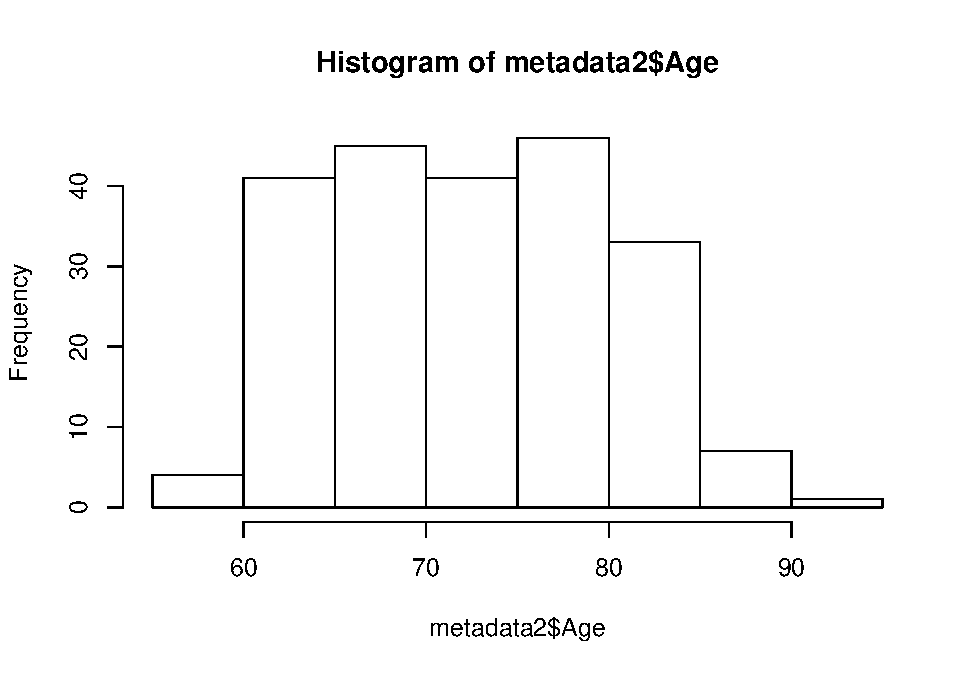
\includegraphics{20180125_summary_to_date_files/figure-latex/unnamed-chunk-62-1.pdf}

Add \emph{apoe4} column

\begin{Shaded}
\begin{Highlighting}[]
\KeywordTok{unique}\NormalTok{(metadata2}\OperatorTok{$}\NormalTok{Demographic.ApoE.genotype)}
\end{Highlighting}
\end{Shaded}

\begin{verbatim}
## [1] E3/E3 E4/E3 E4/E2 E3/E2 E4/E4 E2/E2
## Levels:  E2/E2 E3/E2 E3/E3 E4/E2 E4/E3 E4/E4
\end{verbatim}

\begin{Shaded}
\begin{Highlighting}[]
\NormalTok{metadata2}\OperatorTok{$}\NormalTok{apoe4 <-}\StringTok{ }\KeywordTok{as.factor}\NormalTok{(}\KeywordTok{ifelse}\NormalTok{(metadata2}\OperatorTok{$}\NormalTok{Demographic.ApoE.genotype}\OperatorTok{==}\StringTok{"E2/E2"}\OperatorTok{|}\NormalTok{metadata2}\OperatorTok{$}\NormalTok{Demographic.ApoE.genotype}\OperatorTok{==}\StringTok{"E3/E2"}\OperatorTok{|}\NormalTok{metadata2}\OperatorTok{$}\NormalTok{Demographic.ApoE.genotype}\OperatorTok{==}\StringTok{"E3/E3"}\NormalTok{,}\DecValTok{0}\NormalTok{,}\KeywordTok{ifelse}\NormalTok{(metadata2}\OperatorTok{$}\NormalTok{Demographic.ApoE.genotype}\OperatorTok{==}\StringTok{"E4/E2"}\OperatorTok{|}\NormalTok{metadata2}\OperatorTok{$}\NormalTok{Demographic.ApoE.genotype}\OperatorTok{==}\StringTok{"E4/E3"}\OperatorTok{|}\NormalTok{metadata2}\OperatorTok{$}\NormalTok{Demographic.ApoE.genotype}\OperatorTok{==}\StringTok{"E4/E4"}\NormalTok{,}\DecValTok{1}\NormalTok{,}\OtherTok{NA}\NormalTok{)))}
\NormalTok{metadata2 }\OperatorTok\StringTok{ }
\StringTok{  }\KeywordTok{group_by}\NormalTok{(apoe4) }\OperatorTok\StringTok{ }
\StringTok{  }\KeywordTok{summarise}\NormalTok{(}\DataTypeTok{no_rows =} \KeywordTok{length}\NormalTok{(apoe4))}
\end{Highlighting}
\end{Shaded}

\begin{verbatim}
## # A tibble: 2 x 2
##   apoe4 no_rows
##   <fct>   <int>
## 1 0         115
## 2 1         103
\end{verbatim}

Create binary PET status

\begin{Shaded}
\begin{Highlighting}[]
\NormalTok{metadata2}\OperatorTok{$}\NormalTok{PET <-}\StringTok{ }\KeywordTok{as.factor}\NormalTok{(}\KeywordTok{ifelse}\NormalTok{(metadata2}\OperatorTok{$}\NormalTok{Image.PET.Amyloid.PIB_NAV.Status }\OperatorTok{==}\StringTok{ "Positive"} \OperatorTok{|}\StringTok{ }\NormalTok{metadata2}\OperatorTok{$}\NormalTok{Image.PET.Amyloid.Florbetapir.Status}\OperatorTok{==}\StringTok{ "Positive"} \OperatorTok{|}\StringTok{ }\NormalTok{metadata2}\OperatorTok{$}\NormalTok{Image.PET.Amyloid.Flutemetamol.Status }\OperatorTok{==}\StringTok{ "Positive"}\NormalTok{, }\StringTok{"POS"}\NormalTok{, }\KeywordTok{ifelse}\NormalTok{(metadata2}\OperatorTok{$}\NormalTok{Image.PET.Amyloid.PIB_NAV.Status }\OperatorTok{==}\StringTok{ "Negative"} \OperatorTok{|}\StringTok{ }\NormalTok{metadata2}\OperatorTok{$}\NormalTok{Image.PET.Amyloid.Florbetapir.Status}\OperatorTok{==}\StringTok{ "Negative"} \OperatorTok{|}\StringTok{ }\NormalTok{metadata2}\OperatorTok{$}\NormalTok{Image.PET.Amyloid.Flutemetamol.Status }\OperatorTok{==}\StringTok{ "Negative"}\NormalTok{, }\StringTok{"NEG"}\NormalTok{,}\OtherTok{NA}\NormalTok{)))}
\NormalTok{metadata2 }\OperatorTok\StringTok{ }
\StringTok{  }\KeywordTok{group_by}\NormalTok{(PET) }\OperatorTok\StringTok{ }
\StringTok{  }\KeywordTok{summarise}\NormalTok{(}\DataTypeTok{no_rows =} \KeywordTok{length}\NormalTok{(PET))}
\end{Highlighting}
\end{Shaded}

\begin{verbatim}
## # A tibble: 3 x 2
##   PET   no_rows
##   <fct>   <int>
## 1 NEG        94
## 2 POS       102
## 3 <NA>       22
\end{verbatim}

Extract metadata for columns of interest

\begin{Shaded}
\begin{Highlighting}[]
\NormalTok{meta2 <-}\StringTok{ }\NormalTok{dplyr}\OperatorTok{::}\KeywordTok{select}\NormalTok{(metadata2, }
\NormalTok{                AIBL.Id,}
\NormalTok{                Demographic.Sex,}
\NormalTok{                PET,}
\NormalTok{                apoe4,}
\NormalTok{                Age)}
\KeywordTok{write.table}\NormalTok{(meta2, }\StringTok{"C:/Users/bre227/Documents/R/AD_project/Working/key_metadata.txt"}\NormalTok{, }\DataTypeTok{col.names =}\NormalTok{ T, }\DataTypeTok{row.names =}\NormalTok{ F, }\DataTypeTok{quote =}\NormalTok{ F, }\DataTypeTok{sep =} \StringTok{"}\CharTok{\textbackslash{}t}\StringTok{"}\NormalTok{)}
\end{Highlighting}
\end{Shaded}

\begin{center}\rule{0.5\linewidth}{\linethickness}\end{center}

\subsection{Create initial exploratory
plots}\label{create-initial-exploratory-plots}

Plot for whole dataset

\begin{Shaded}
\begin{Highlighting}[]
\NormalTok{exdata1 <-}\StringTok{ }\KeywordTok{as_tibble}\NormalTok{(exdata)}
\NormalTok{exdata1 <-}\StringTok{ }\KeywordTok{as_tibble}\NormalTok{(}\KeywordTok{t}\NormalTok{(exdata1)) }\CommentTok{# transpose to put samples in rows, genes in columns}
\KeywordTok{colnames}\NormalTok{(exdata1) <-}\StringTok{ }\KeywordTok{rownames}\NormalTok{(exdata) }\CommentTok{# add genes names}
\NormalTok{exdata1}\OperatorTok{$}\NormalTok{AIBL.Id <-}\StringTok{ }\KeywordTok{as.integer}\NormalTok{(}\KeywordTok{colnames}\NormalTok{(exdata)) }\CommentTok{# add 'AIBL.Id' column}
\NormalTok{exdata2 <-}\StringTok{ }\KeywordTok{left_join}\NormalTok{(meta2, exdata1, }\DataTypeTok{by =} \StringTok{"AIBL.Id"}\NormalTok{) }\OperatorTok\StringTok{ }
\StringTok{  }\NormalTok{na.omit }\CommentTok{# add metadata and remove PET and apoe4 columns with 'NA'}
\KeywordTok{rownames}\NormalTok{(exdata2) <-}\StringTok{ }\NormalTok{exdata2}\OperatorTok{$}\NormalTok{AIBL.Id }\CommentTok{# to ensure the labels in the plots reflect the AIBL.Ids}
\KeywordTok{dim}\NormalTok{(exdata2)}
\end{Highlighting}
\end{Shaded}

\begin{verbatim}
## [1]   196 22016
\end{verbatim}

Run PCA

\begin{Shaded}
\begin{Highlighting}[]
\NormalTok{pca <-}\StringTok{ }\KeywordTok{prcomp}\NormalTok{(exdata2[}\DecValTok{6}\OperatorTok{:}\DecValTok{22016}\NormalTok{], }\DataTypeTok{center =}\NormalTok{ T, }\DataTypeTok{scale. =}\NormalTok{ T) }\CommentTok{# run PCA}
\CommentTok{# plot scree for PCA}
\KeywordTok{library}\NormalTok{(factoextra)}
\KeywordTok{fviz_eig}\NormalTok{(pca)}
\end{Highlighting}
\end{Shaded}

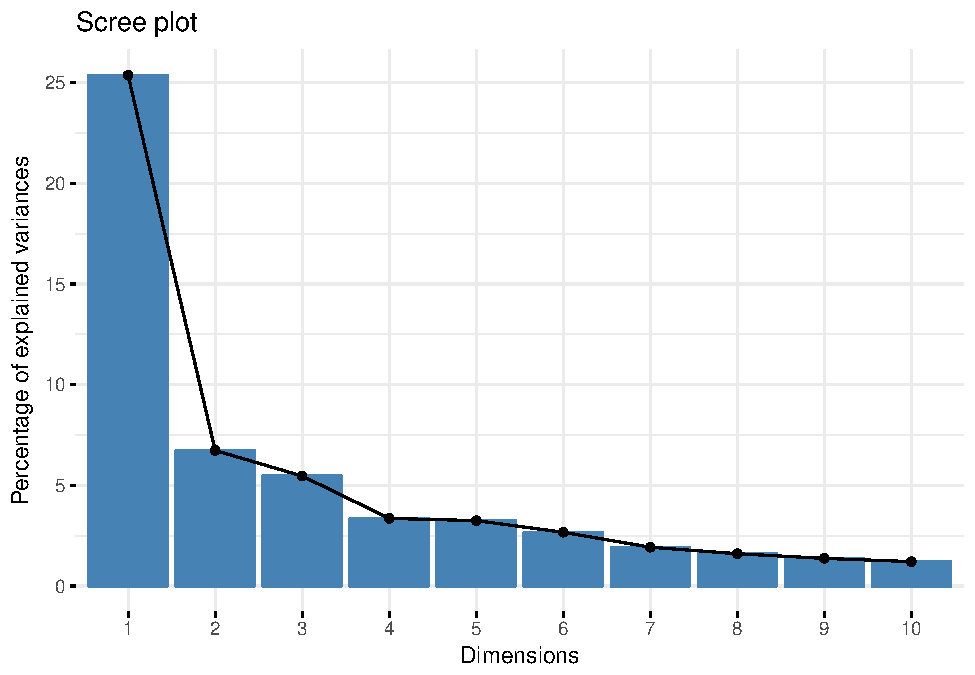
\includegraphics{20180125_summary_to_date_files/figure-latex/unnamed-chunk-67-1.pdf}

PCA scatterplot for PET status

\begin{Shaded}
\begin{Highlighting}[]
\KeywordTok{library}\NormalTok{(ggfortify)}
\KeywordTok{autoplot}\NormalTok{(pca, }\DataTypeTok{data =}\NormalTok{ exdata2, }\DataTypeTok{colour =} \StringTok{"PET"}\NormalTok{, }\DataTypeTok{label =}\NormalTok{ T) }\OperatorTok{+}
\StringTok{  }\NormalTok{viridis}\OperatorTok{::}\KeywordTok{scale_colour_viridis}\NormalTok{(}\DataTypeTok{option =} \StringTok{"viridis"}\NormalTok{, }\DataTypeTok{discrete =}\NormalTok{ T)}
\end{Highlighting}
\end{Shaded}

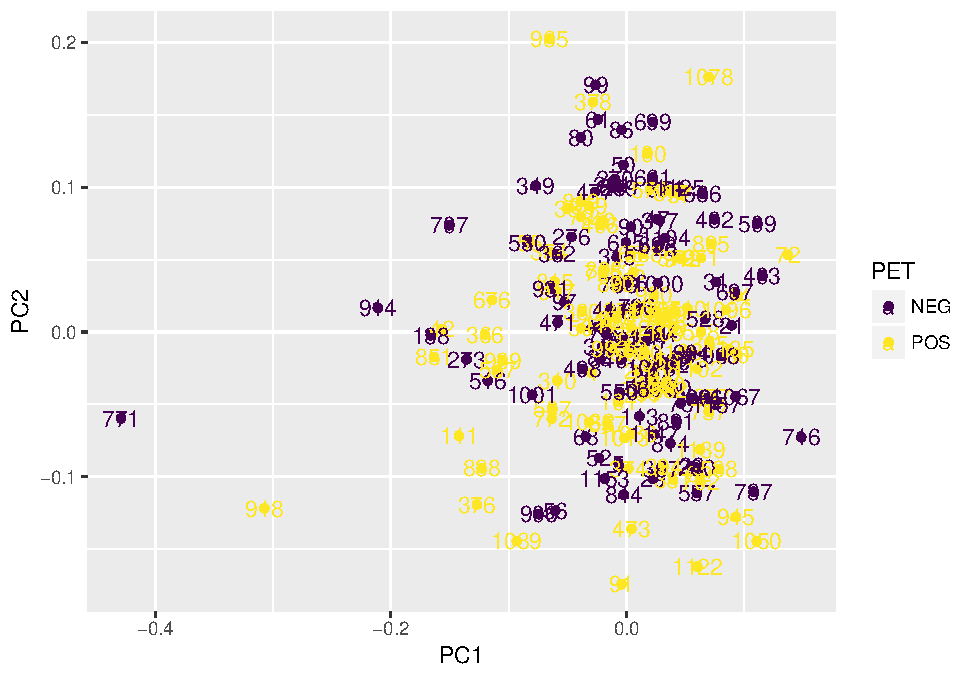
\includegraphics{20180125_summary_to_date_files/figure-latex/unnamed-chunk-68-1.pdf}

PET scatterplot for \emph{apoe4} status

\begin{Shaded}
\begin{Highlighting}[]
\KeywordTok{library}\NormalTok{(ggfortify)}
\KeywordTok{autoplot}\NormalTok{(pca, }\DataTypeTok{data =}\NormalTok{ exdata2, }\DataTypeTok{colour =} \StringTok{"apoe4"}\NormalTok{, }\DataTypeTok{label =}\NormalTok{ T)}
\end{Highlighting}
\end{Shaded}

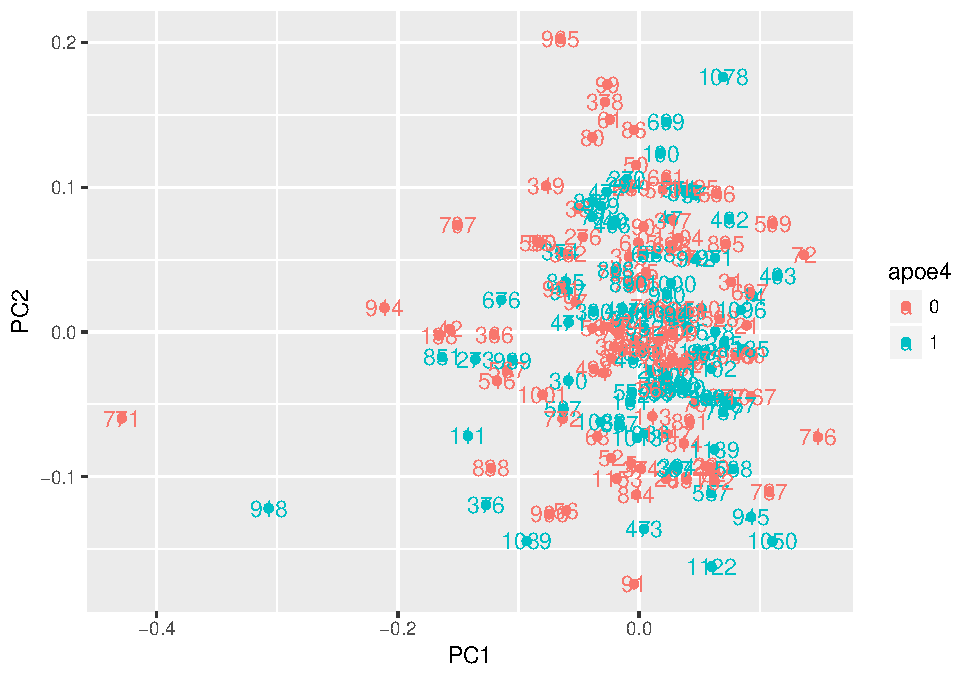
\includegraphics{20180125_summary_to_date_files/figure-latex/unnamed-chunk-69-1.pdf}

\begin{Shaded}
\begin{Highlighting}[]
\KeywordTok{qqnorm}\NormalTok{(pca}\OperatorTok{$}\NormalTok{x[,}\DecValTok{2}\NormalTok{], }\DataTypeTok{pch =} \DecValTok{20}\NormalTok{)}
\end{Highlighting}
\end{Shaded}

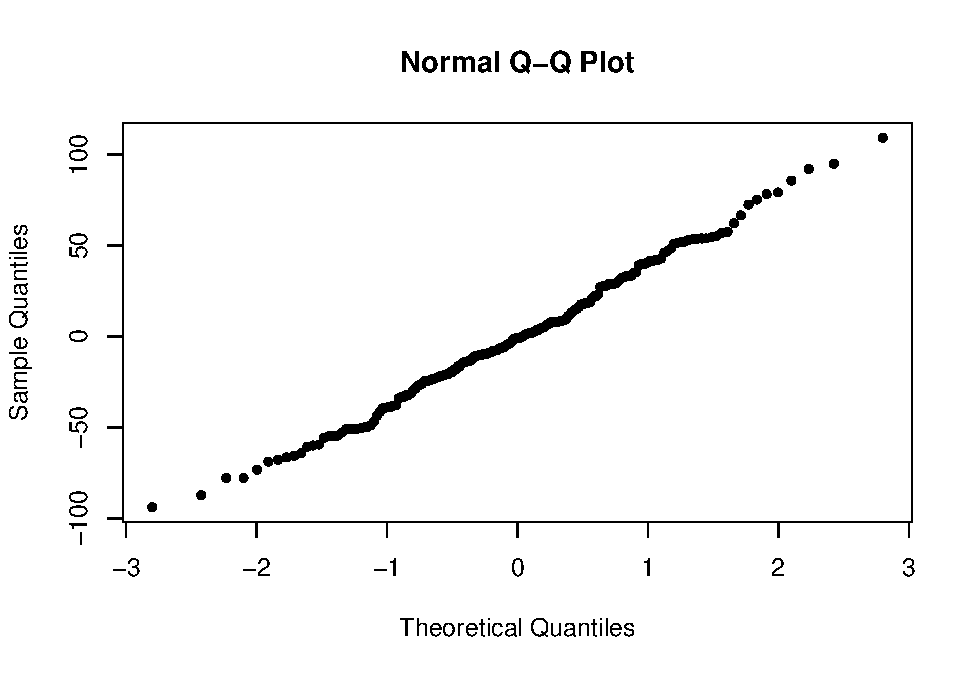
\includegraphics{20180125_summary_to_date_files/figure-latex/unnamed-chunk-70-1.pdf}

Exclude outliers and run PCA again

\begin{Shaded}
\begin{Highlighting}[]
\NormalTok{exdata3 <-}\StringTok{ }\KeywordTok{filter}\NormalTok{(exdata2, AIBL.Id }\OperatorTok{!=}\StringTok{ "771"} \OperatorTok{&}\StringTok{ }\NormalTok{AIBL.Id }\OperatorTok{!=}\StringTok{ "914"} \OperatorTok{&}\StringTok{ }\NormalTok{AIBL.Id }\OperatorTok{!=}\StringTok{ "918"}\NormalTok{)}
\end{Highlighting}
\end{Shaded}

Run PCA

\begin{Shaded}
\begin{Highlighting}[]
\NormalTok{pca2 <-}\StringTok{ }\KeywordTok{prcomp}\NormalTok{(exdata3[}\DecValTok{6}\OperatorTok{:}\DecValTok{22016}\NormalTok{], }\DataTypeTok{center =}\NormalTok{ T, }\DataTypeTok{scale. =}\NormalTok{ T) }\CommentTok{# run PCA}
\KeywordTok{library}\NormalTok{(factoextra)}
\KeywordTok{fviz_eig}\NormalTok{(pca2)}
\end{Highlighting}
\end{Shaded}

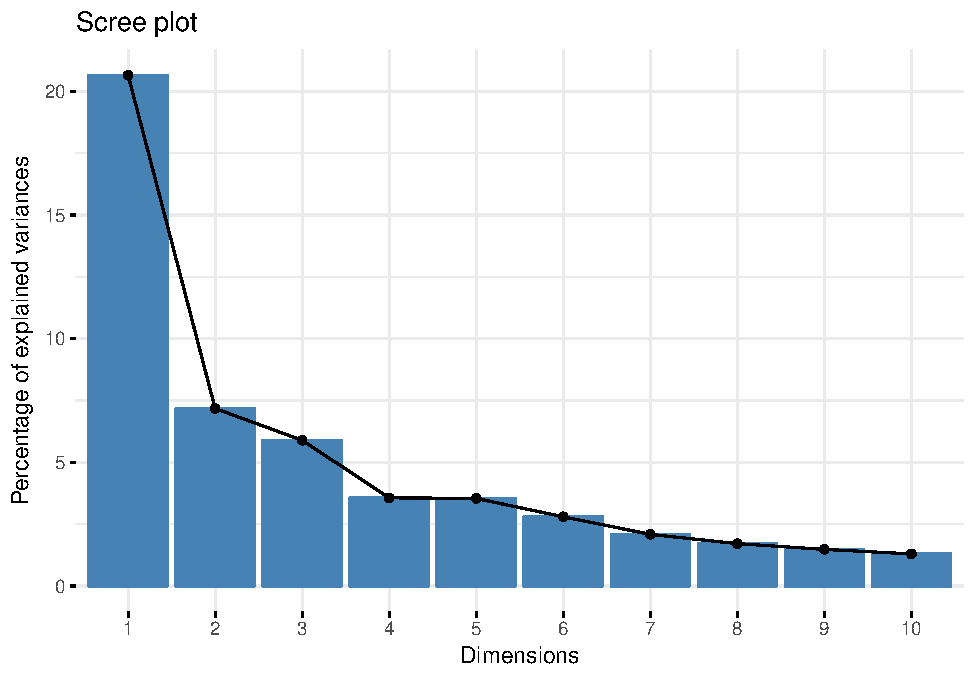
\includegraphics{20180125_summary_to_date_files/figure-latex/unnamed-chunk-72-1.pdf}

Plot without outliers (PET)

\begin{Shaded}
\begin{Highlighting}[]
\KeywordTok{library}\NormalTok{(ggfortify)}
\KeywordTok{autoplot}\NormalTok{(pca2, }\DataTypeTok{data =}\NormalTok{ exdata3, }\DataTypeTok{colour =} \StringTok{"PET"}\NormalTok{, }\DataTypeTok{label =}\NormalTok{ T, }\DataTypeTok{label.label =} \StringTok{"AIBL.Id"}\NormalTok{) }\OperatorTok{+}
\StringTok{  }\NormalTok{viridis}\OperatorTok{::}\KeywordTok{scale_colour_viridis}\NormalTok{(}\DataTypeTok{option =} \StringTok{"viridis"}\NormalTok{, }\DataTypeTok{discrete =}\NormalTok{ T)}
\end{Highlighting}
\end{Shaded}

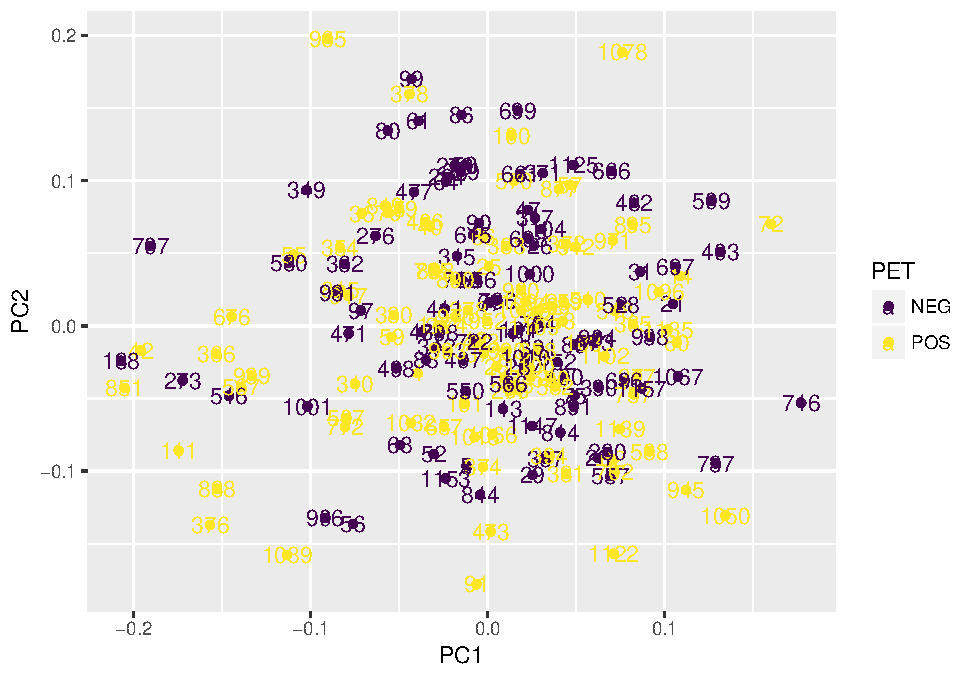
\includegraphics{20180125_summary_to_date_files/figure-latex/unnamed-chunk-73-1.pdf}

Plot without outliers (\emph{apoe4})

\begin{Shaded}
\begin{Highlighting}[]
\KeywordTok{library}\NormalTok{(ggfortify)}
\KeywordTok{autoplot}\NormalTok{(pca2, }\DataTypeTok{data =}\NormalTok{ exdata3, }\DataTypeTok{colour =} \StringTok{"apoe4"}\NormalTok{, }\DataTypeTok{label =}\NormalTok{ T, }\DataTypeTok{label.label =} \StringTok{"AIBL.Id"}\NormalTok{)}
\end{Highlighting}
\end{Shaded}

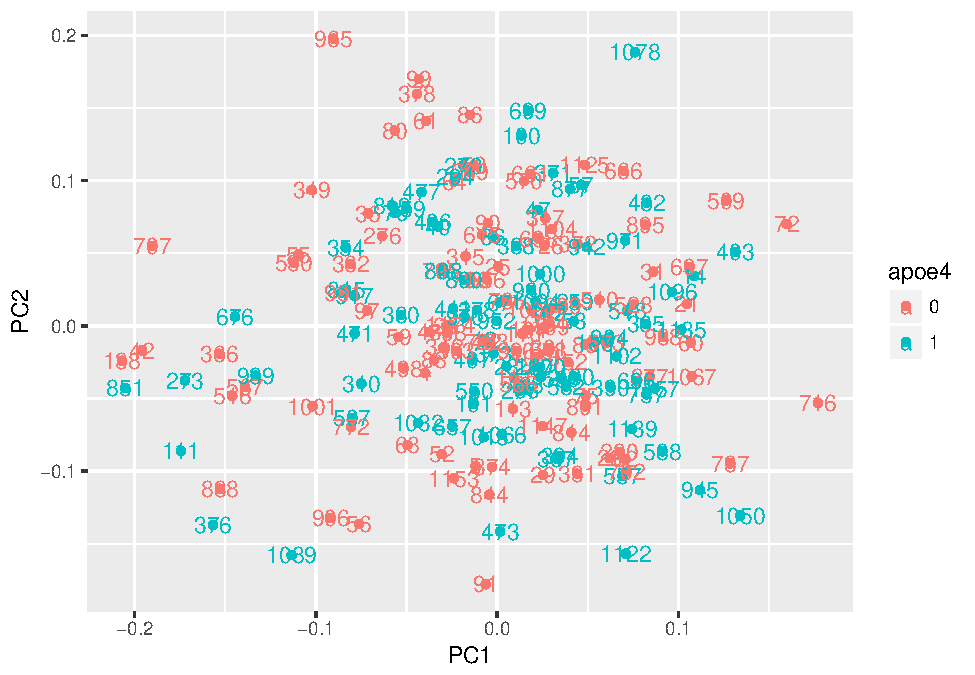
\includegraphics{20180125_summary_to_date_files/figure-latex/unnamed-chunk-74-1.pdf}

\begin{center}\rule{0.5\linewidth}{\linethickness}\end{center}

\subsection{\texorpdfstring{Use \texttt{limma} to analyse expression
data.}{Use limma to analyse expression data.}}\label{use-limma-to-analyse-expression-data.}

We first create an `ExpressionSet' with genes on rows, and samples on
columns, following the guide here:
\url{https://www.bioconductor.org/packages/3.7/bioc/vignettes/Biobase/inst/doc/ExpressionSetIntroduction.pdf}

\begin{Shaded}
\begin{Highlighting}[]
\KeywordTok{library}\NormalTok{(Biobase)}
\end{Highlighting}
\end{Shaded}

\begin{Shaded}
\begin{Highlighting}[]
\NormalTok{exprs <-}\StringTok{ }\KeywordTok{as.matrix}\NormalTok{(}\KeywordTok{t}\NormalTok{(exdata3[,}\DecValTok{6}\OperatorTok{:}\DecValTok{22016}\NormalTok{])) }\CommentTok{# leaving behind the first 5 metadata columns}
\NormalTok{minimalSet <-}\StringTok{ }\KeywordTok{ExpressionSet}\NormalTok{(}\DataTypeTok{assayData =}\NormalTok{ exprs)}
\NormalTok{pData <-}\StringTok{ }\NormalTok{exdata3[,}\DecValTok{1}\OperatorTok{:}\DecValTok{5}\NormalTok{]}
\KeywordTok{summary}\NormalTok{(pData)}
\end{Highlighting}
\end{Shaded}

\begin{verbatim}
##     AIBL.Id       Demographic.Sex  PET      apoe4        Age       
##  Min.   :   4.0   Female:96       NEG: 92   0:105   Min.   :55.15  
##  1st Qu.: 110.0   Male  :97       POS:101   1: 88   1st Qu.:67.15  
##  Median : 480.0                                     Median :72.71  
##  Mean   : 506.2                                     Mean   :72.86  
##  3rd Qu.: 819.0                                     3rd Qu.:78.90  
##  Max.   :1174.0                                     Max.   :91.79
\end{verbatim}

\begin{Shaded}
\begin{Highlighting}[]
\KeywordTok{library}\NormalTok{(limma)}
\end{Highlighting}
\end{Shaded}

\begin{Shaded}
\begin{Highlighting}[]
\NormalTok{PET_apoe4 <-}\StringTok{ }\KeywordTok{paste}\NormalTok{(pData}\OperatorTok{$}\NormalTok{PET, pData}\OperatorTok{$}\NormalTok{apoe4, }\DataTypeTok{sep =} \StringTok{"."}\NormalTok{) }\CommentTok{# put PET/apoe4 combinations into a vector}

\NormalTok{PET_apoe4 <-}\StringTok{ }\KeywordTok{factor}\NormalTok{(PET_apoe4, }\DataTypeTok{levels =} \KeywordTok{c}\NormalTok{(}\KeywordTok{unique}\NormalTok{(PET_apoe4))) }\CommentTok{# turn it into a factor}
\NormalTok{design <-}\StringTok{ }\KeywordTok{model.matrix}\NormalTok{(}\OperatorTok{~}\DecValTok{0} \OperatorTok{+}\StringTok{ }\NormalTok{PET_apoe4) }\CommentTok{# create factor table for four combinations}
\KeywordTok{colnames}\NormalTok{(design) <-}\StringTok{ }\KeywordTok{levels}\NormalTok{(PET_apoe4)}
\NormalTok{fit <-}\StringTok{ }\KeywordTok{lmFit}\NormalTok{(exprs, design)}
\end{Highlighting}
\end{Shaded}

Set four pair-wise contrasts of interest and compute the contrasts and
moderated t-tests.

\begin{Shaded}
\begin{Highlighting}[]
\NormalTok{cont.matrix <-}\StringTok{ }\KeywordTok{makeContrasts}\NormalTok{(}\DataTypeTok{apoe4_for_PET_yes =}\NormalTok{ POS.}\DecValTok{1} \OperatorTok{-}\StringTok{ }\NormalTok{POS.}\DecValTok{0}\NormalTok{,}
                             \DataTypeTok{apoe4_for_PET_no =}\NormalTok{ NEG.}\DecValTok{1} \OperatorTok{-}\StringTok{ }\NormalTok{NEG.}\DecValTok{0}\NormalTok{,}
                             \DataTypeTok{PET_for_apoe4_yes =}\NormalTok{ POS.}\DecValTok{1} \OperatorTok{-}\StringTok{ }\NormalTok{NEG.}\DecValTok{1}\NormalTok{,}
                             \DataTypeTok{PET_for_apoe4_no =}\NormalTok{ POS.}\DecValTok{0} \OperatorTok{-}\StringTok{ }\NormalTok{NEG.}\DecValTok{0}\NormalTok{,}
                             \DataTypeTok{levels =}\NormalTok{ design)}
\NormalTok{fit2 <-}\StringTok{ }\KeywordTok{contrasts.fit}\NormalTok{(fit, cont.matrix)}
\NormalTok{fit2 <-}\StringTok{ }\KeywordTok{eBayes}\NormalTok{(fit2)}
\end{Highlighting}
\end{Shaded}

Get the genes differentially expressed in each comparison

\begin{Shaded}
\begin{Highlighting}[]
\NormalTok{res1 <-}\StringTok{ }\KeywordTok{topTable}\NormalTok{(fit2, }\DataTypeTok{coef =} \StringTok{"apoe4_for_PET_yes"}\NormalTok{, }\DataTypeTok{n =} \OtherTok{Inf}\NormalTok{)}
\NormalTok{res2 <-}\StringTok{ }\KeywordTok{topTable}\NormalTok{(fit2, }\DataTypeTok{coef =} \StringTok{"apoe4_for_PET_no"}\NormalTok{, }\DataTypeTok{n =} \OtherTok{Inf}\NormalTok{)}
\NormalTok{res3 <-}\StringTok{ }\KeywordTok{topTable}\NormalTok{(fit2, }\DataTypeTok{coef =} \StringTok{"PET_for_apoe4_yes"}\NormalTok{, }\DataTypeTok{n =} \OtherTok{Inf}\NormalTok{)}
\NormalTok{res4 <-}\StringTok{ }\KeywordTok{topTable}\NormalTok{(fit2, }\DataTypeTok{coef =} \StringTok{"PET_for_apoe4_no"}\NormalTok{, }\DataTypeTok{n =} \OtherTok{Inf}\NormalTok{)}

\KeywordTok{length}\NormalTok{(}\KeywordTok{which}\NormalTok{(res1}\OperatorTok{$}\NormalTok{P.Value }\OperatorTok{<}\StringTok{ }\FloatTok{0.05}\NormalTok{))}
\end{Highlighting}
\end{Shaded}

\begin{verbatim}
## [1] 653
\end{verbatim}

\begin{Shaded}
\begin{Highlighting}[]
\KeywordTok{length}\NormalTok{(}\KeywordTok{which}\NormalTok{(res2}\OperatorTok{$}\NormalTok{P.Value }\OperatorTok{<}\StringTok{ }\FloatTok{0.05}\NormalTok{))}
\end{Highlighting}
\end{Shaded}

\begin{verbatim}
## [1] 684
\end{verbatim}

\begin{Shaded}
\begin{Highlighting}[]
\KeywordTok{length}\NormalTok{(}\KeywordTok{which}\NormalTok{(res3}\OperatorTok{$}\NormalTok{P.Value }\OperatorTok{<}\StringTok{ }\FloatTok{0.05}\NormalTok{))}
\end{Highlighting}
\end{Shaded}

\begin{verbatim}
## [1] 924
\end{verbatim}

\begin{Shaded}
\begin{Highlighting}[]
\KeywordTok{length}\NormalTok{(}\KeywordTok{which}\NormalTok{(res4}\OperatorTok{$}\NormalTok{P.Value }\OperatorTok{<}\StringTok{ }\FloatTok{0.05}\NormalTok{))}
\end{Highlighting}
\end{Shaded}

\begin{verbatim}
## [1] 769
\end{verbatim}

Probe IDs are set in the `res' data frames as rownames. Create separate
column for rownames. Need to do it now, because when \texttt{filter()}
is applied below, it removes the rownames.

\begin{Shaded}
\begin{Highlighting}[]
\ControlFlowTok{for}\NormalTok{ (i }\ControlFlowTok{in} \KeywordTok{ls}\NormalTok{(}\DataTypeTok{pattern =} \StringTok{"res"}\NormalTok{))\{}
\NormalTok{  x <-}\StringTok{ }\KeywordTok{get}\NormalTok{(i)}
\NormalTok{  x}\OperatorTok{$}\NormalTok{probe_id <-}\StringTok{ }\KeywordTok{rownames}\NormalTok{(x)}
  \KeywordTok{assign}\NormalTok{(i, x)}
\NormalTok{\}}
\end{Highlighting}
\end{Shaded}

Get list of genes that show significantly different expression between
contrasts

\begin{Shaded}
\begin{Highlighting}[]
\NormalTok{signif_apoe4_for_PET_yes <-}\StringTok{ }\KeywordTok{filter}\NormalTok{(res1, P.Value }\OperatorTok{<}\StringTok{ }\FloatTok{0.05}\NormalTok{)}
\NormalTok{signif_apoe4_for_PET_no <-}\StringTok{ }\KeywordTok{filter}\NormalTok{(res2, P.Value }\OperatorTok{<}\StringTok{ }\FloatTok{0.05}\NormalTok{)}
\NormalTok{signif_PET_for_apoe4_yes <-}\StringTok{ }\KeywordTok{filter}\NormalTok{(res3, P.Value }\OperatorTok{<}\StringTok{ }\FloatTok{0.05}\NormalTok{)}
\NormalTok{signif_PET_for_apoe4_no <-}\StringTok{ }\KeywordTok{filter}\NormalTok{(res4, P.Value }\OperatorTok{<}\StringTok{ }\FloatTok{0.05}\NormalTok{)}

\KeywordTok{rm}\NormalTok{(}\DataTypeTok{list =} \KeywordTok{ls}\NormalTok{(}\DataTypeTok{pattern =} \StringTok{"res"}\NormalTok{)) }\CommentTok{# remove results to clear working memory}
\end{Highlighting}
\end{Shaded}

\subsection{Get gene identifiers for microarray probes and identify
significant
genes.}\label{get-gene-identifiers-for-microarray-probes-and-identify-significant-genes.}

\emph{Using JD's code from `AIBL\_Gene\_Expression\_SetUp\_Dec82017.R'}

\begin{Shaded}
\begin{Highlighting}[]
\KeywordTok{library}\NormalTok{(pd.huex.}\FloatTok{1.0}\NormalTok{.st.v2)}
\KeywordTok{library}\NormalTok{(huex10sttranscriptcluster.db)}
  
\NormalTok{### pull gene symbols and match to probe ids to replace rownames }\AlertTok{###}
\NormalTok{x <-}\StringTok{ }\NormalTok{huex10sttranscriptclusterSYMBOL}
\CommentTok{# Get the probe identifiers that are mapped to a gene symbol}
\NormalTok{mapped_probes <-}\StringTok{ }\KeywordTok{mappedkeys}\NormalTok{(x)}
\CommentTok{# Convert to a list}
\NormalTok{xx <-}\StringTok{ }\KeywordTok{as.list}\NormalTok{(x[mapped_probes])}
\ControlFlowTok{if}\NormalTok{(}\KeywordTok{length}\NormalTok{(xx) }\OperatorTok{>}\StringTok{ }\DecValTok{0}\NormalTok{) \{}
\CommentTok{# Get the SYMBOL for the first five probes}
\NormalTok{xx[}\DecValTok{1}\OperatorTok{:}\DecValTok{5}\NormalTok{]}
\CommentTok{# Get the first one}
\NormalTok{xx[[}\DecValTok{1}\NormalTok{]]}
\NormalTok{\}}
\end{Highlighting}
\end{Shaded}

\begin{verbatim}
## [1] "LOC102723600"
\end{verbatim}

\begin{Shaded}
\begin{Highlighting}[]
\NormalTok{xx1 <-}\StringTok{ }\KeywordTok{as.matrix}\NormalTok{(}\KeywordTok{unlist}\NormalTok{(xx))}

\CommentTok{# Get table of probes}
\NormalTok{gns <-}\StringTok{ }\KeywordTok{rownames}\NormalTok{(exdata)}
\NormalTok{gnsl <-}\StringTok{ }\NormalTok{xx1[}\KeywordTok{rownames}\NormalTok{(xx1) }\OperatorTok\StringTok{ }\NormalTok{gns]}
\KeywordTok{length}\NormalTok{(gnsl)}
\end{Highlighting}
\end{Shaded}

\begin{verbatim}
## [1] 14825
\end{verbatim}

\begin{Shaded}
\begin{Highlighting}[]
\NormalTok{### Find ENSEMBL IDs }\AlertTok{###}
\NormalTok{x3 <-}\StringTok{ }\NormalTok{huex10sttranscriptclusterENSEMBL}
\CommentTok{# Get the entrez gene IDs that are mapped to an Ensembl ID}
\NormalTok{mapped_genes <-}\StringTok{ }\KeywordTok{mappedkeys}\NormalTok{(x3)}
\CommentTok{# Convert to a list}
\NormalTok{xx3 <-}\StringTok{ }\KeywordTok{as.list}\NormalTok{(x3[mapped_genes])}

\NormalTok{xx3.}\DecValTok{1}\NormalTok{ <-}\StringTok{ }\KeywordTok{as.matrix}\NormalTok{(}\KeywordTok{unlist}\NormalTok{(xx3))}
\NormalTok{ens <-}\StringTok{ }\NormalTok{xx3.}\DecValTok{1}\NormalTok{[}\KeywordTok{rownames}\NormalTok{(xx3.}\DecValTok{1}\NormalTok{) }\OperatorTok\StringTok{ }\NormalTok{gns]}
\KeywordTok{length}\NormalTok{(ens)}
\end{Highlighting}
\end{Shaded}

\begin{verbatim}
## [1] 13991
\end{verbatim}

\begin{Shaded}
\begin{Highlighting}[]
\CommentTok{#[1] 14497}

\NormalTok{### Find Entrez IDs }\AlertTok{###}
\NormalTok{x4 <-}\StringTok{ }\NormalTok{huex10sttranscriptclusterENTREZID}
\CommentTok{# Get the probe identifiers that are mapped to an ENTREZ Gene ID}
\NormalTok{mapped_probes <-}\StringTok{ }\KeywordTok{mappedkeys}\NormalTok{(x4)}
\CommentTok{# Convert to a list}
\NormalTok{xx4 <-}\StringTok{ }\KeywordTok{as.list}\NormalTok{(x4[mapped_probes])}

\NormalTok{xx4.}\DecValTok{1}\NormalTok{ <-}\StringTok{ }\KeywordTok{as.matrix}\NormalTok{(}\KeywordTok{unlist}\NormalTok{(xx4))}
\NormalTok{entz <-}\StringTok{ }\NormalTok{xx4.}\DecValTok{1}\NormalTok{[}\KeywordTok{rownames}\NormalTok{(xx4.}\DecValTok{1}\NormalTok{) }\OperatorTok\StringTok{ }\NormalTok{gns]}
\KeywordTok{length}\NormalTok{(entz)}
\end{Highlighting}
\end{Shaded}

\begin{verbatim}
## [1] 14825
\end{verbatim}

\subsection{Match probes, gene symbols, Ensembl IDs, and Entrez IDs with
the list of statistically significant
genes.}\label{match-probes-gene-symbols-ensembl-ids-and-entrez-ids-with-the-list-of-statistically-significant-genes.}

Create data frame of all probe matches with identifiers

\begin{Shaded}
\begin{Highlighting}[]
\NormalTok{pid_symb <-}\StringTok{  }\KeywordTok{data.frame}\NormalTok{(xx1)}
\NormalTok{pid_symb}\OperatorTok{$}\NormalTok{probe_id <-}\StringTok{ }\KeywordTok{rownames}\NormalTok{(pid_symb)}

\NormalTok{pid_ens <-}\StringTok{ }\KeywordTok{data.frame}\NormalTok{(xx3.}\DecValTok{1}\NormalTok{)}
\NormalTok{pid_ens}\OperatorTok{$}\NormalTok{probe_id <-}\StringTok{ }\KeywordTok{rownames}\NormalTok{(pid_ens)}

\NormalTok{pid_ent <-}\StringTok{ }\KeywordTok{data.frame}\NormalTok{(xx4.}\DecValTok{1}\NormalTok{)}
\NormalTok{pid_ent}\OperatorTok{$}\NormalTok{probe_id <-}\StringTok{ }\KeywordTok{rownames}\NormalTok{(pid_ent)}

\NormalTok{pid_all <-}\StringTok{ }\KeywordTok{left_join}\NormalTok{(pid_symb, pid_ent, }\DataTypeTok{by =} \StringTok{"probe_id"}\NormalTok{) }\OperatorTok\StringTok{ }
\StringTok{  }\KeywordTok{left_join}\NormalTok{(}\DataTypeTok{y =}\NormalTok{ pid_ens, }\DataTypeTok{by =} \StringTok{"probe_id"}\NormalTok{) }\OperatorTok\StringTok{ }
\StringTok{  }\KeywordTok{rename}\NormalTok{(}\DataTypeTok{xx1 =} \StringTok{"gene_symbol"}\NormalTok{,}
         \DataTypeTok{xx4.1 =} \StringTok{"entrez_id"}\NormalTok{,}
         \DataTypeTok{xx3.1 =} \StringTok{"ensembl_id"}\NormalTok{) }\OperatorTok\StringTok{ }
\StringTok{  }\NormalTok{dplyr}\OperatorTok{::}\KeywordTok{select}\NormalTok{(probe_id, }\KeywordTok{everything}\NormalTok{())}

\KeywordTok{write.table}\NormalTok{(pid_all, }\StringTok{"C:/Users/bre227/Documents/R/AD_project/Working/affy_probes_annotated.txt"}\NormalTok{, }\DataTypeTok{row.names =}\NormalTok{ F, }\DataTypeTok{col.names =}\NormalTok{ T, }\DataTypeTok{quote =}\NormalTok{ F, }\DataTypeTok{sep =} \StringTok{"}\CharTok{\textbackslash{}t}\StringTok{"}\NormalTok{)}

\CommentTok{# find how many probes are annotated}
\KeywordTok{length}\NormalTok{(}\KeywordTok{which}\NormalTok{(pid_all}\OperatorTok{$}\NormalTok{probe_id }\OperatorTok\StringTok{ }\KeywordTok{rownames}\NormalTok{(exdata)))}
\end{Highlighting}
\end{Shaded}

\begin{verbatim}
## [1] 14825
\end{verbatim}

Combine lists of significant genes for each contrast. Note that combined
counts of significant genes for all four contrasts is 3030.

\begin{Shaded}
\begin{Highlighting}[]
\NormalTok{signif_all <-}\StringTok{ }\KeywordTok{full_join}\NormalTok{(signif_apoe4_for_PET_yes, signif_apoe4_for_PET_no, }\DataTypeTok{by =} \StringTok{"probe_id"}\NormalTok{) }\OperatorTok
\StringTok{  }\KeywordTok{full_join}\NormalTok{(signif_PET_for_apoe4_no, }\DataTypeTok{by =} \StringTok{"probe_id"}\NormalTok{) }\OperatorTok\StringTok{ }
\StringTok{  }\KeywordTok{full_join}\NormalTok{(signif_apoe4_for_PET_yes, }\DataTypeTok{by =} \StringTok{"probe_id"}\NormalTok{)}

\NormalTok{signif_all <-}\StringTok{ }\NormalTok{dplyr}\OperatorTok{::}\KeywordTok{select}\NormalTok{(signif_apoe4_for_PET_yes, probe_id, P.Value) }\OperatorTok\StringTok{ }
\StringTok{  }\KeywordTok{full_join}\NormalTok{(dplyr}\OperatorTok{::}\KeywordTok{select}\NormalTok{(signif_apoe4_for_PET_no, probe_id, P.Value), }\DataTypeTok{by =} \StringTok{"probe_id"}\NormalTok{) }\OperatorTok\StringTok{ }
\StringTok{  }\KeywordTok{full_join}\NormalTok{(dplyr}\OperatorTok{::}\KeywordTok{select}\NormalTok{(signif_PET_for_apoe4_yes, probe_id, P.Value), }\DataTypeTok{by =} \StringTok{"probe_id"}\NormalTok{) }\OperatorTok\StringTok{ }
\StringTok{  }\KeywordTok{full_join}\NormalTok{(dplyr}\OperatorTok{::}\KeywordTok{select}\NormalTok{(signif_PET_for_apoe4_no, probe_id, P.Value), }\DataTypeTok{by =} \StringTok{"probe_id"}\NormalTok{) }\OperatorTok\StringTok{ }
\StringTok{  }\KeywordTok{rename}\NormalTok{(}\DataTypeTok{P.Value.x =} \StringTok{"P.Value.c1"}\NormalTok{, }
         \DataTypeTok{P.Value.y =} \StringTok{"P.Value.c2"}\NormalTok{, }
         \DataTypeTok{P.Value.x.x =} \StringTok{"P.Value.c3"}\NormalTok{, }
         \DataTypeTok{P.Value.y.y =} \StringTok{"P.Value.c4"}\NormalTok{)}

\KeywordTok{nrow}\NormalTok{(signif_all)}
\end{Highlighting}
\end{Shaded}

\begin{verbatim}
## [1] 2438
\end{verbatim}

Therefore 2438 genes are expressed differentially across at least two
contrasts

Bind gene ids to `signif\_all'

\begin{Shaded}
\begin{Highlighting}[]
\NormalTok{sig_all2 <-}\StringTok{ }\KeywordTok{left_join}\NormalTok{(signif_all, pid_all, }\DataTypeTok{by =} \StringTok{"probe_id"}\NormalTok{)}
\end{Highlighting}
\end{Shaded}

There are many NAs in the `gene\_symbol' column, even though there are
34,127 unique probe\_ids in `pid\_symb' - one would think they would all
be accounted for.

\begin{Shaded}
\begin{Highlighting}[]
\KeywordTok{length}\NormalTok{(}\KeywordTok{setdiff}\NormalTok{(signif_all}\OperatorTok{$}\NormalTok{probe_id, pid_all}\OperatorTok{$}\NormalTok{probe_id))}
\end{Highlighting}
\end{Shaded}

\begin{verbatim}
## [1] 1000
\end{verbatim}

Shows that there are 1000 probe ids in `signif\_all' that are not in
`pid\_all', i.e.~they do not have any annotation data.

Confirmed by:

\begin{Shaded}
\begin{Highlighting}[]
\KeywordTok{length}\NormalTok{(}\KeywordTok{which}\NormalTok{(signif_all}\OperatorTok{$}\NormalTok{probe_id }\OperatorTok\StringTok{ }\NormalTok{pid_all}\OperatorTok{$}\NormalTok{probe_id }\OperatorTok{==}\StringTok{ "TRUE"}\NormalTok{))}
\end{Highlighting}
\end{Shaded}

\begin{verbatim}
## [1] 1438
\end{verbatim}

So are all probe\_ids in the expression data in `pid\_symb'?

\begin{Shaded}
\begin{Highlighting}[]
\KeywordTok{length}\NormalTok{(}\KeywordTok{setdiff}\NormalTok{(}\KeywordTok{rownames}\NormalTok{(exdata), pid_symb}\OperatorTok{$}\NormalTok{probe_id))}
\end{Highlighting}
\end{Shaded}

\begin{verbatim}
## [1] 7186
\end{verbatim}

7,186/22,011 probes are not accounted for in the annotation data?

Confirm this:

\begin{Shaded}
\begin{Highlighting}[]
\KeywordTok{length}\NormalTok{(}\KeywordTok{which}\NormalTok{(}\KeywordTok{rownames}\NormalTok{(exdata) }\OperatorTok\StringTok{ }\NormalTok{pid_all}\OperatorTok{$}\NormalTok{probe_id }\OperatorTok{==}\StringTok{ "TRUE"}\NormalTok{))}
\end{Highlighting}
\end{Shaded}

\begin{verbatim}
## [1] 14825
\end{verbatim}

\paragraph{Venn diagram of overlapping
genes}\label{venn-diagram-of-overlapping-genes}

\begin{Shaded}
\begin{Highlighting}[]
\KeywordTok{library}\NormalTok{(VennDiagram)}
\KeywordTok{grid.newpage}\NormalTok{()}
\NormalTok{venn <-}\StringTok{ }\KeywordTok{draw.quad.venn}\NormalTok{(}\DataTypeTok{area1 =} \KeywordTok{length}\NormalTok{(}\KeywordTok{which}\NormalTok{(}\OperatorTok{!}\KeywordTok{is.na}\NormalTok{(sig_all2}\OperatorTok{$}\NormalTok{P.Value.c1))),}
               \DataTypeTok{area2 =} \KeywordTok{length}\NormalTok{(}\KeywordTok{which}\NormalTok{(}\OperatorTok{!}\KeywordTok{is.na}\NormalTok{(sig_all2}\OperatorTok{$}\NormalTok{P.Value.c2))),}
               \DataTypeTok{area3 =} \KeywordTok{length}\NormalTok{(}\KeywordTok{which}\NormalTok{(}\OperatorTok{!}\KeywordTok{is.na}\NormalTok{(sig_all2}\OperatorTok{$}\NormalTok{P.Value.c3))),}
               \DataTypeTok{area4 =} \KeywordTok{length}\NormalTok{(}\KeywordTok{which}\NormalTok{(}\OperatorTok{!}\KeywordTok{is.na}\NormalTok{(sig_all2}\OperatorTok{$}\NormalTok{P.Value.c4))),}
               \DataTypeTok{n12 =} \KeywordTok{length}\NormalTok{(}\KeywordTok{which}\NormalTok{(}\OperatorTok{!}\KeywordTok{is.na}\NormalTok{(sig_all2}\OperatorTok{$}\NormalTok{P.Value.c1) }\OperatorTok{&}\StringTok{ }\OperatorTok{!}\KeywordTok{is.na}\NormalTok{(sig_all2}\OperatorTok{$}\NormalTok{P.Value.c2))),}
               \DataTypeTok{n13 =} \KeywordTok{length}\NormalTok{(}\KeywordTok{which}\NormalTok{(}\OperatorTok{!}\KeywordTok{is.na}\NormalTok{(sig_all2}\OperatorTok{$}\NormalTok{P.Value.c1) }\OperatorTok{&}\StringTok{ }\OperatorTok{!}\KeywordTok{is.na}\NormalTok{(sig_all2}\OperatorTok{$}\NormalTok{P.Value.c3))),}
               \DataTypeTok{n14 =} \KeywordTok{length}\NormalTok{(}\KeywordTok{which}\NormalTok{(}\OperatorTok{!}\KeywordTok{is.na}\NormalTok{(sig_all2}\OperatorTok{$}\NormalTok{P.Value.c1) }\OperatorTok{&}\StringTok{ }\OperatorTok{!}\KeywordTok{is.na}\NormalTok{(sig_all2}\OperatorTok{$}\NormalTok{P.Value.c4))),}
               \DataTypeTok{n23 =} \KeywordTok{length}\NormalTok{(}\KeywordTok{which}\NormalTok{(}\OperatorTok{!}\KeywordTok{is.na}\NormalTok{(sig_all2}\OperatorTok{$}\NormalTok{P.Value.c2) }\OperatorTok{&}\StringTok{ }\OperatorTok{!}\KeywordTok{is.na}\NormalTok{(sig_all2}\OperatorTok{$}\NormalTok{P.Value.c3))),}
               \DataTypeTok{n24 =} \KeywordTok{length}\NormalTok{(}\KeywordTok{which}\NormalTok{(}\OperatorTok{!}\KeywordTok{is.na}\NormalTok{(sig_all2}\OperatorTok{$}\NormalTok{P.Value.c2) }\OperatorTok{&}\StringTok{ }\OperatorTok{!}\KeywordTok{is.na}\NormalTok{(sig_all2}\OperatorTok{$}\NormalTok{P.Value.c4))),}
               \DataTypeTok{n34 =} \KeywordTok{length}\NormalTok{(}\KeywordTok{which}\NormalTok{(}\OperatorTok{!}\KeywordTok{is.na}\NormalTok{(sig_all2}\OperatorTok{$}\NormalTok{P.Value.c3) }\OperatorTok{&}\StringTok{ }\OperatorTok{!}\KeywordTok{is.na}\NormalTok{(sig_all2}\OperatorTok{$}\NormalTok{P.Value.c4))),}
               \DataTypeTok{n123 =} \KeywordTok{length}\NormalTok{(}\KeywordTok{which}\NormalTok{(}\OperatorTok{!}\KeywordTok{is.na}\NormalTok{(sig_all2}\OperatorTok{$}\NormalTok{P.Value.c1) }\OperatorTok{&}\StringTok{ }\OperatorTok{!}\KeywordTok{is.na}\NormalTok{(sig_all2}\OperatorTok{$}\NormalTok{P.Value.c2) }\OperatorTok{&}\StringTok{ }\OperatorTok{!}\KeywordTok{is.na}\NormalTok{(sig_all2}\OperatorTok{$}\NormalTok{P.Value.c3))),}
               \DataTypeTok{n124 =} \KeywordTok{length}\NormalTok{(}\KeywordTok{which}\NormalTok{(}\OperatorTok{!}\KeywordTok{is.na}\NormalTok{(sig_all2}\OperatorTok{$}\NormalTok{P.Value.c1) }\OperatorTok{&}\StringTok{ }\OperatorTok{!}\KeywordTok{is.na}\NormalTok{(sig_all2}\OperatorTok{$}\NormalTok{P.Value.c2) }\OperatorTok{&}\StringTok{ }\OperatorTok{!}\KeywordTok{is.na}\NormalTok{(sig_all2}\OperatorTok{$}\NormalTok{P.Value.c4))),}
               \DataTypeTok{n134 =} \KeywordTok{length}\NormalTok{(}\KeywordTok{which}\NormalTok{(}\OperatorTok{!}\KeywordTok{is.na}\NormalTok{(sig_all2}\OperatorTok{$}\NormalTok{P.Value.c1) }\OperatorTok{&}\StringTok{ }\OperatorTok{!}\KeywordTok{is.na}\NormalTok{(sig_all2}\OperatorTok{$}\NormalTok{P.Value.c3) }\OperatorTok{&}\StringTok{ }\OperatorTok{!}\KeywordTok{is.na}\NormalTok{(sig_all2}\OperatorTok{$}\NormalTok{P.Value.c4))),}
               \DataTypeTok{n234 =} \KeywordTok{length}\NormalTok{(}\KeywordTok{which}\NormalTok{(}\OperatorTok{!}\KeywordTok{is.na}\NormalTok{(sig_all2}\OperatorTok{$}\NormalTok{P.Value.c2) }\OperatorTok{&}\StringTok{ }\OperatorTok{!}\KeywordTok{is.na}\NormalTok{(sig_all2}\OperatorTok{$}\NormalTok{P.Value.c3) }\OperatorTok{&}\StringTok{ }\OperatorTok{!}\KeywordTok{is.na}\NormalTok{(sig_all2}\OperatorTok{$}\NormalTok{P.Value.c4))), }
               \DataTypeTok{n1234 =} \KeywordTok{length}\NormalTok{(}\KeywordTok{which}\NormalTok{(}\OperatorTok{!}\KeywordTok{is.na}\NormalTok{(sig_all2}\OperatorTok{$}\NormalTok{P.Value.c1) }\OperatorTok{&}\StringTok{ }\OperatorTok{!}\KeywordTok{is.na}\NormalTok{(sig_all2}\OperatorTok{$}\NormalTok{P.Value.c2) }\OperatorTok{&}\StringTok{ }\OperatorTok{!}\KeywordTok{is.na}\NormalTok{(sig_all2}\OperatorTok{$}\NormalTok{P.Value.c3) }\OperatorTok{&}\StringTok{ }\OperatorTok{!}\KeywordTok{is.na}\NormalTok{(sig_all2}\OperatorTok{$}\NormalTok{P.Value.c4))),}
               \DataTypeTok{category =} \KeywordTok{c}\NormalTok{(}\StringTok{"apoe4_for_PET_yes"}\NormalTok{, }\StringTok{"apoe4_for_PET_no"}\NormalTok{, }\StringTok{"PET_for_apoe4_yes"}\NormalTok{, }\StringTok{"PET_for_apoe4_no"}\NormalTok{),}
               \DataTypeTok{cat.pos =} \KeywordTok{c}\NormalTok{(}\DecValTok{0}\NormalTok{, }\DecValTok{0}\NormalTok{, }\DecValTok{0}\NormalTok{, }\DecValTok{0}\NormalTok{))}
\end{Highlighting}
\end{Shaded}

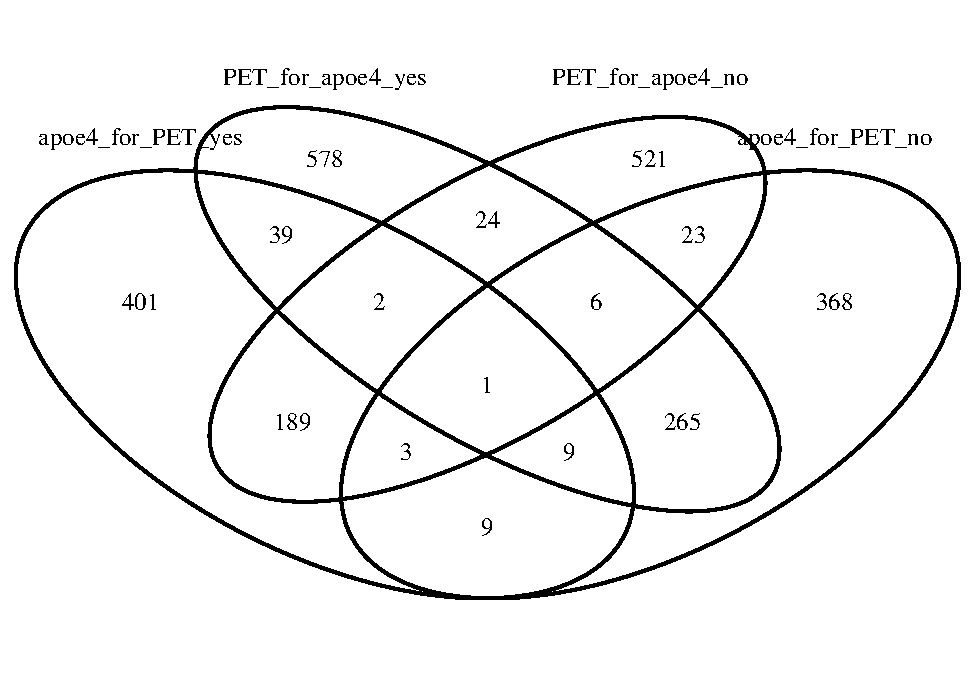
\includegraphics{20180125_summary_to_date_files/figure-latex/unnamed-chunk-91-1.pdf}

Many of the same genes (265) are differentially expressed between: * PET
pos/neg when they have the apoe4 allele; and * apoe4 yes/no when they
are negative for PET

These could be genes that can protect against AD.

Many of the same genes (189) are also differentially expressed between:
* PET pos/neg when they do not have the apoe4 allele; and * apoe4 yes/no
when they are positive for PET

These latter genes must be acting independently of the apoe4 network to
cause AD.

Find out how many people are in each group:

\begin{Shaded}
\begin{Highlighting}[]
\NormalTok{test <-}\StringTok{ }\NormalTok{exdata3[,}\DecValTok{1}\OperatorTok{:}\DecValTok{5}\NormalTok{]}
\KeywordTok{length}\NormalTok{(}\KeywordTok{which}\NormalTok{(test}\OperatorTok{$}\NormalTok{PET }\OperatorTok{==}\StringTok{ "POS"} \OperatorTok{&}\StringTok{ }\NormalTok{test}\OperatorTok{$}\NormalTok{apoe4 }\OperatorTok{==}\StringTok{ "1"}\NormalTok{))}
\end{Highlighting}
\end{Shaded}

\begin{verbatim}
## [1] 65
\end{verbatim}

\begin{Shaded}
\begin{Highlighting}[]
\KeywordTok{length}\NormalTok{(}\KeywordTok{which}\NormalTok{(test}\OperatorTok{$}\NormalTok{PET }\OperatorTok{==}\StringTok{ "POS"} \OperatorTok{&}\StringTok{ }\NormalTok{test}\OperatorTok{$}\NormalTok{apoe4 }\OperatorTok{==}\StringTok{ "0"}\NormalTok{))}
\end{Highlighting}
\end{Shaded}

\begin{verbatim}
## [1] 36
\end{verbatim}

\begin{Shaded}
\begin{Highlighting}[]
\KeywordTok{length}\NormalTok{(}\KeywordTok{which}\NormalTok{(test}\OperatorTok{$}\NormalTok{PET }\OperatorTok{==}\StringTok{ "NEG"} \OperatorTok{&}\StringTok{ }\NormalTok{test}\OperatorTok{$}\NormalTok{apoe4 }\OperatorTok{==}\StringTok{ "1"}\NormalTok{))}
\end{Highlighting}
\end{Shaded}

\begin{verbatim}
## [1] 23
\end{verbatim}

\begin{Shaded}
\begin{Highlighting}[]
\KeywordTok{length}\NormalTok{(}\KeywordTok{which}\NormalTok{(test}\OperatorTok{$}\NormalTok{PET }\OperatorTok{==}\StringTok{ "NEG"} \OperatorTok{&}\StringTok{ }\NormalTok{test}\OperatorTok{$}\NormalTok{apoe4 }\OperatorTok{==}\StringTok{ "0"}\NormalTok{))}
\end{Highlighting}
\end{Shaded}

\begin{verbatim}
## [1] 69
\end{verbatim}

This suggests that more people tend to either have apoe4 and AD, or not
have apoe4 and not have AD, than otherwise.

\begin{center}\rule{0.5\linewidth}{\linethickness}\end{center}

\subsection{Compare expression profiles between PET-pos and PET-neg
groups}\label{compare-expression-profiles-between-pet-pos-and-pet-neg-groups}

Create design matrix

\begin{Shaded}
\begin{Highlighting}[]
\NormalTok{Group <-}\StringTok{ }\KeywordTok{factor}\NormalTok{(exdata3}\OperatorTok{$}\NormalTok{PET, }\DataTypeTok{levels =} \KeywordTok{c}\NormalTok{(}\StringTok{"POS"}\NormalTok{, }\StringTok{"NEG"}\NormalTok{))}
\NormalTok{design2 <-}\StringTok{ }\KeywordTok{model.matrix}\NormalTok{(}\OperatorTok{~}\DecValTok{0} \OperatorTok{+}\StringTok{ }\NormalTok{Group)}
\KeywordTok{colnames}\NormalTok{(design2) <-}\StringTok{ }\KeywordTok{c}\NormalTok{(}\StringTok{"POS"}\NormalTok{, }\StringTok{"NEG"}\NormalTok{)}
\end{Highlighting}
\end{Shaded}

Find differentially expressed genes

\begin{Shaded}
\begin{Highlighting}[]
\NormalTok{fit3 <-}\StringTok{ }\KeywordTok{lmFit}\NormalTok{(exprs, design2)}
\NormalTok{cont.matrix2 <-}\StringTok{ }\KeywordTok{makeContrasts}\NormalTok{(}\DataTypeTok{POSvsNEG =}\NormalTok{ POS }\OperatorTok{-}\StringTok{ }\NormalTok{NEG, }\DataTypeTok{levels =}\NormalTok{ design2)}
\NormalTok{fit4 <-}\StringTok{ }\KeywordTok{contrasts.fit}\NormalTok{(fit3, cont.matrix2)}
\NormalTok{fit4 <-}\StringTok{ }\KeywordTok{eBayes}\NormalTok{(fit4)}
\KeywordTok{topTable}\NormalTok{(fit4, }\DataTypeTok{adjust =} \StringTok{"BH"}\NormalTok{)}
\end{Highlighting}
\end{Shaded}

\begin{verbatim}
##               logFC  AveExpr         t      P.Value adj.P.Val           B
## 2328611 -0.24349043 6.931149 -3.781354 0.0002074070 0.9997102  0.50013583
## 3997946  0.14334623 9.035701  3.648961 0.0003381087 0.9997102  0.07930919
## 2566383 -0.08138720 8.334744 -3.626837 0.0003664051 0.9997102  0.01024134
## 2694314  0.10608542 6.813847  3.553376 0.0004772006 0.9997102 -0.21648884
## 3707258  0.06258903 6.911761  3.470792 0.0006390722 0.9997102 -0.46656387
## 3957224  0.08050569 6.324961  3.469708 0.0006415049 0.9997102 -0.46981262
## 3934479  0.07847492 6.465840  3.468142 0.0006450341 0.9997102 -0.47450352
## 3819771  0.21167767 5.350143  3.463788 0.0006549411 0.9997102 -0.48753481
## 3462630 -0.07185294 3.382152 -3.439265 0.0007134666 0.9997102 -0.56067593
## 4038494  0.10130047 3.711608  3.427094 0.0007442989 0.9997102 -0.59680772
\end{verbatim}

\begin{Shaded}
\begin{Highlighting}[]
\NormalTok{results_PETposvneg <-}\StringTok{ }\KeywordTok{topTable}\NormalTok{(fit4, }\DataTypeTok{n =} \OtherTok{Inf}\NormalTok{)}
\NormalTok{results_PETposvneg}\OperatorTok{$}\NormalTok{probe_id <-}\StringTok{ }\KeywordTok{rownames}\NormalTok{(results_PETposvneg)}
\NormalTok{signif_PET_pos_v_neg <-}\StringTok{ }\KeywordTok{filter}\NormalTok{(results_PETposvneg, P.Value }\OperatorTok{<}\StringTok{ }\FloatTok{0.05}\NormalTok{)}
\KeywordTok{dim}\NormalTok{(signif_PET_pos_v_neg)}
\end{Highlighting}
\end{Shaded}

\begin{verbatim}
## [1] 865   7
\end{verbatim}

Now for apoe4

\begin{Shaded}
\begin{Highlighting}[]
\NormalTok{Group <-}\StringTok{ }\KeywordTok{factor}\NormalTok{(exdata3}\OperatorTok{$}\NormalTok{apoe4, }\DataTypeTok{levels =} \KeywordTok{c}\NormalTok{(}\DecValTok{0}\NormalTok{, }\DecValTok{1}\NormalTok{))}
\NormalTok{design3 <-}\StringTok{ }\KeywordTok{model.matrix}\NormalTok{(}\OperatorTok{~}\DecValTok{0} \OperatorTok{+}\StringTok{ }\NormalTok{Group)}
\KeywordTok{colnames}\NormalTok{(design3) <-}\StringTok{ }\KeywordTok{c}\NormalTok{(}\StringTok{"NEG"}\NormalTok{, }\StringTok{"POS"}\NormalTok{)}
\end{Highlighting}
\end{Shaded}

Find differentially expressed genes

\begin{Shaded}
\begin{Highlighting}[]
\NormalTok{fit5 <-}\StringTok{ }\KeywordTok{lmFit}\NormalTok{(exprs, design3)}
\NormalTok{cont.matrix3 <-}\StringTok{ }\KeywordTok{makeContrasts}\NormalTok{(}\DataTypeTok{apoe4 =}\NormalTok{ NEG }\OperatorTok{-}\StringTok{ }\NormalTok{POS, }\DataTypeTok{levels =}\NormalTok{ design3)}
\NormalTok{fit6 <-}\StringTok{ }\KeywordTok{contrasts.fit}\NormalTok{(fit5, cont.matrix3)}
\NormalTok{fit6 <-}\StringTok{ }\KeywordTok{eBayes}\NormalTok{(fit6)}
\KeywordTok{topTable}\NormalTok{(fit6, }\DataTypeTok{adjust =} \StringTok{"BH"}\NormalTok{)}
\end{Highlighting}
\end{Shaded}

\begin{verbatim}
##               logFC  AveExpr         t      P.Value adj.P.Val           B
## 3360287  0.17135398 6.377782  4.107229 5.892379e-05 0.9997616  1.58861565
## 3453446  0.20354250 4.358425  3.702309 2.781176e-04 0.9997616  0.24693729
## 3275398  0.27781363 6.503623  3.643283 3.451692e-04 0.9997616  0.06124851
## 3749570  0.18071224 6.920419  3.505805 5.650003e-04 0.9997616 -0.36123353
## 3450180 -0.08479851 5.565530 -3.475845 6.278481e-04 0.9997616 -0.45142875
## 3719456  0.15291395 3.122911  3.416413 7.723809e-04 0.9997616 -0.62834664
## 3150579 -0.15573427 5.935585 -3.391778 8.409687e-04 0.9997616 -0.70089559
## 2777276  0.07471033 4.025781  3.335889 1.018232e-03 0.9997616 -0.86377471
## 2342904  0.09381612 5.328055  3.331353 1.034053e-03 0.9997616 -0.87689050
## 2432714 -0.20563079 6.724809 -3.232473 1.441337e-03 0.9997616 -1.15884979
\end{verbatim}

\begin{Shaded}
\begin{Highlighting}[]
\NormalTok{results_apoe4posvneg <-}\StringTok{ }\KeywordTok{topTable}\NormalTok{(fit6, }\DataTypeTok{n =} \OtherTok{Inf}\NormalTok{)}
\NormalTok{results_apoe4posvneg}\OperatorTok{$}\NormalTok{probe_id <-}\StringTok{ }\KeywordTok{rownames}\NormalTok{(results_apoe4posvneg)}
\NormalTok{signif_apoe4_pos_v_neg <-}\StringTok{ }\KeywordTok{filter}\NormalTok{(results_apoe4posvneg, P.Value }\OperatorTok{<}\StringTok{ }\FloatTok{0.05}\NormalTok{)}
\KeywordTok{dim}\NormalTok{(signif_apoe4_pos_v_neg)}
\end{Highlighting}
\end{Shaded}

\begin{verbatim}
## [1] 554   7
\end{verbatim}

Create table of all significant differentially expressed genes

\begin{Shaded}
\begin{Highlighting}[]
\NormalTok{sig_direct_pairs <-}\StringTok{ }\KeywordTok{full_join}\NormalTok{(}
\NormalTok{  dplyr}\OperatorTok{::}\KeywordTok{select}\NormalTok{(signif_PET_pos_v_neg, P.Value, probe_id),}
\NormalTok{  dplyr}\OperatorTok{::}\KeywordTok{select}\NormalTok{(signif_apoe4_pos_v_neg, P.Value, probe_id), }
  \DataTypeTok{by =} \StringTok{"probe_id"}\NormalTok{) }\OperatorTok\StringTok{ }
\StringTok{  }\NormalTok{dplyr}\OperatorTok{::}\KeywordTok{select}\NormalTok{(probe_id, }\KeywordTok{everything}\NormalTok{())}
\KeywordTok{colnames}\NormalTok{(sig_direct_pairs)[}\DecValTok{2}\NormalTok{] <-}\StringTok{ "P.Value_PET"}
\KeywordTok{colnames}\NormalTok{(sig_direct_pairs)[}\DecValTok{3}\NormalTok{] <-}\StringTok{ "P.Value_apoe4"}
\end{Highlighting}
\end{Shaded}

\begin{Shaded}
\begin{Highlighting}[]
\KeywordTok{library}\NormalTok{(VennDiagram)}
\KeywordTok{grid.newpage}\NormalTok{()}
\NormalTok{venn2 <-}\StringTok{ }\KeywordTok{draw.pairwise.venn}\NormalTok{(}
  \DataTypeTok{area1 =} \KeywordTok{length}\NormalTok{(}\KeywordTok{which}\NormalTok{(}\OperatorTok{!}\KeywordTok{is.na}\NormalTok{(sig_direct_pairs}\OperatorTok{$}\NormalTok{P.Value_PET))),}
  \DataTypeTok{area2 =} \KeywordTok{length}\NormalTok{(}\KeywordTok{which}\NormalTok{(}\OperatorTok{!}\KeywordTok{is.na}\NormalTok{(sig_direct_pairs}\OperatorTok{$}\NormalTok{P.Value_apoe4))),}
  \DataTypeTok{cross.area =} \KeywordTok{length}\NormalTok{(}\KeywordTok{which}\NormalTok{(}\OperatorTok{!}\KeywordTok{is.na}\NormalTok{(sig_direct_pairs}\OperatorTok{$}\NormalTok{P.Value_PET) }\OperatorTok{&}\StringTok{ }\OperatorTok{!}\KeywordTok{is.na}\NormalTok{(sig_direct_pairs}\OperatorTok{$}\NormalTok{P.Value_apoe4))),}
  \DataTypeTok{category =} \KeywordTok{c}\NormalTok{(}\StringTok{"PET_pos_v_neg"}\NormalTok{, }\StringTok{"apoe4_pos_v_neg"}\NormalTok{),}
  \DataTypeTok{ext.text =} \OtherTok{FALSE}\NormalTok{, }\DataTypeTok{cat.prompts =}\NormalTok{ T, }\DataTypeTok{cat.pos =} \DecValTok{0}\NormalTok{)}
\end{Highlighting}
\end{Shaded}

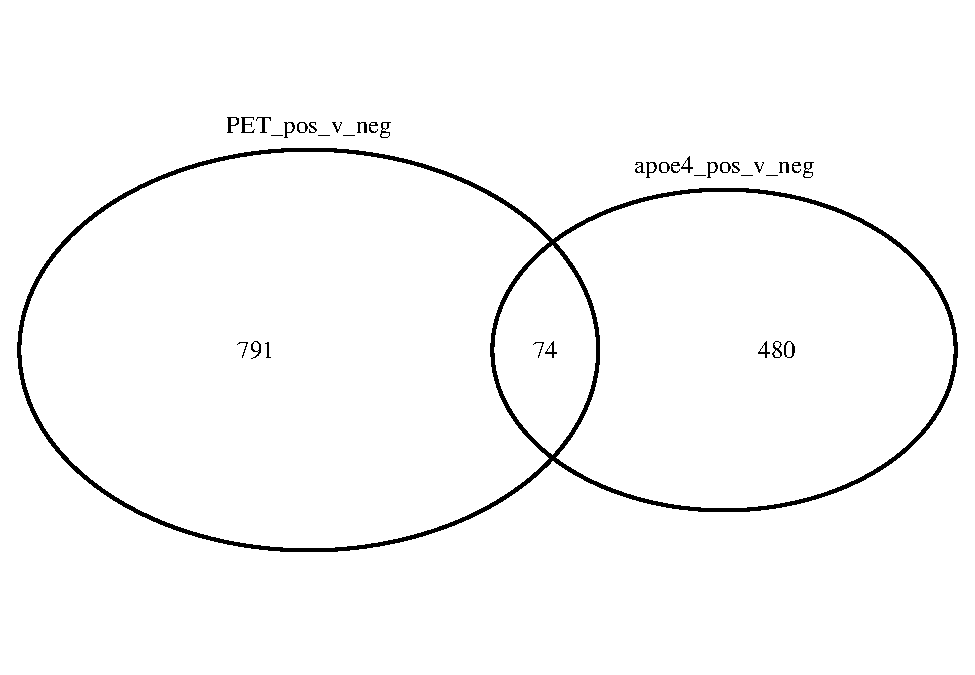
\includegraphics{20180125_summary_to_date_files/figure-latex/unnamed-chunk-100-1.pdf}

\begin{verbatim}
## INFO [2018-01-25 19:09:08] Placing category labels at default outer locations.  Use 'cat.pos' and 'cat.dist' to modify location.
## INFO [2018-01-25 19:09:08] Current 'cat.pos': 0 degrees, 0 degrees
## INFO [2018-01-25 19:09:08] Current 'cat.dist': 0.025 , 0.025
\end{verbatim}


\end{document}
